\section{Results}
\section{Interpolated Dielectric Function $\varepsilon(\omega,T)$}
%
\begin{figure}
    \centering
    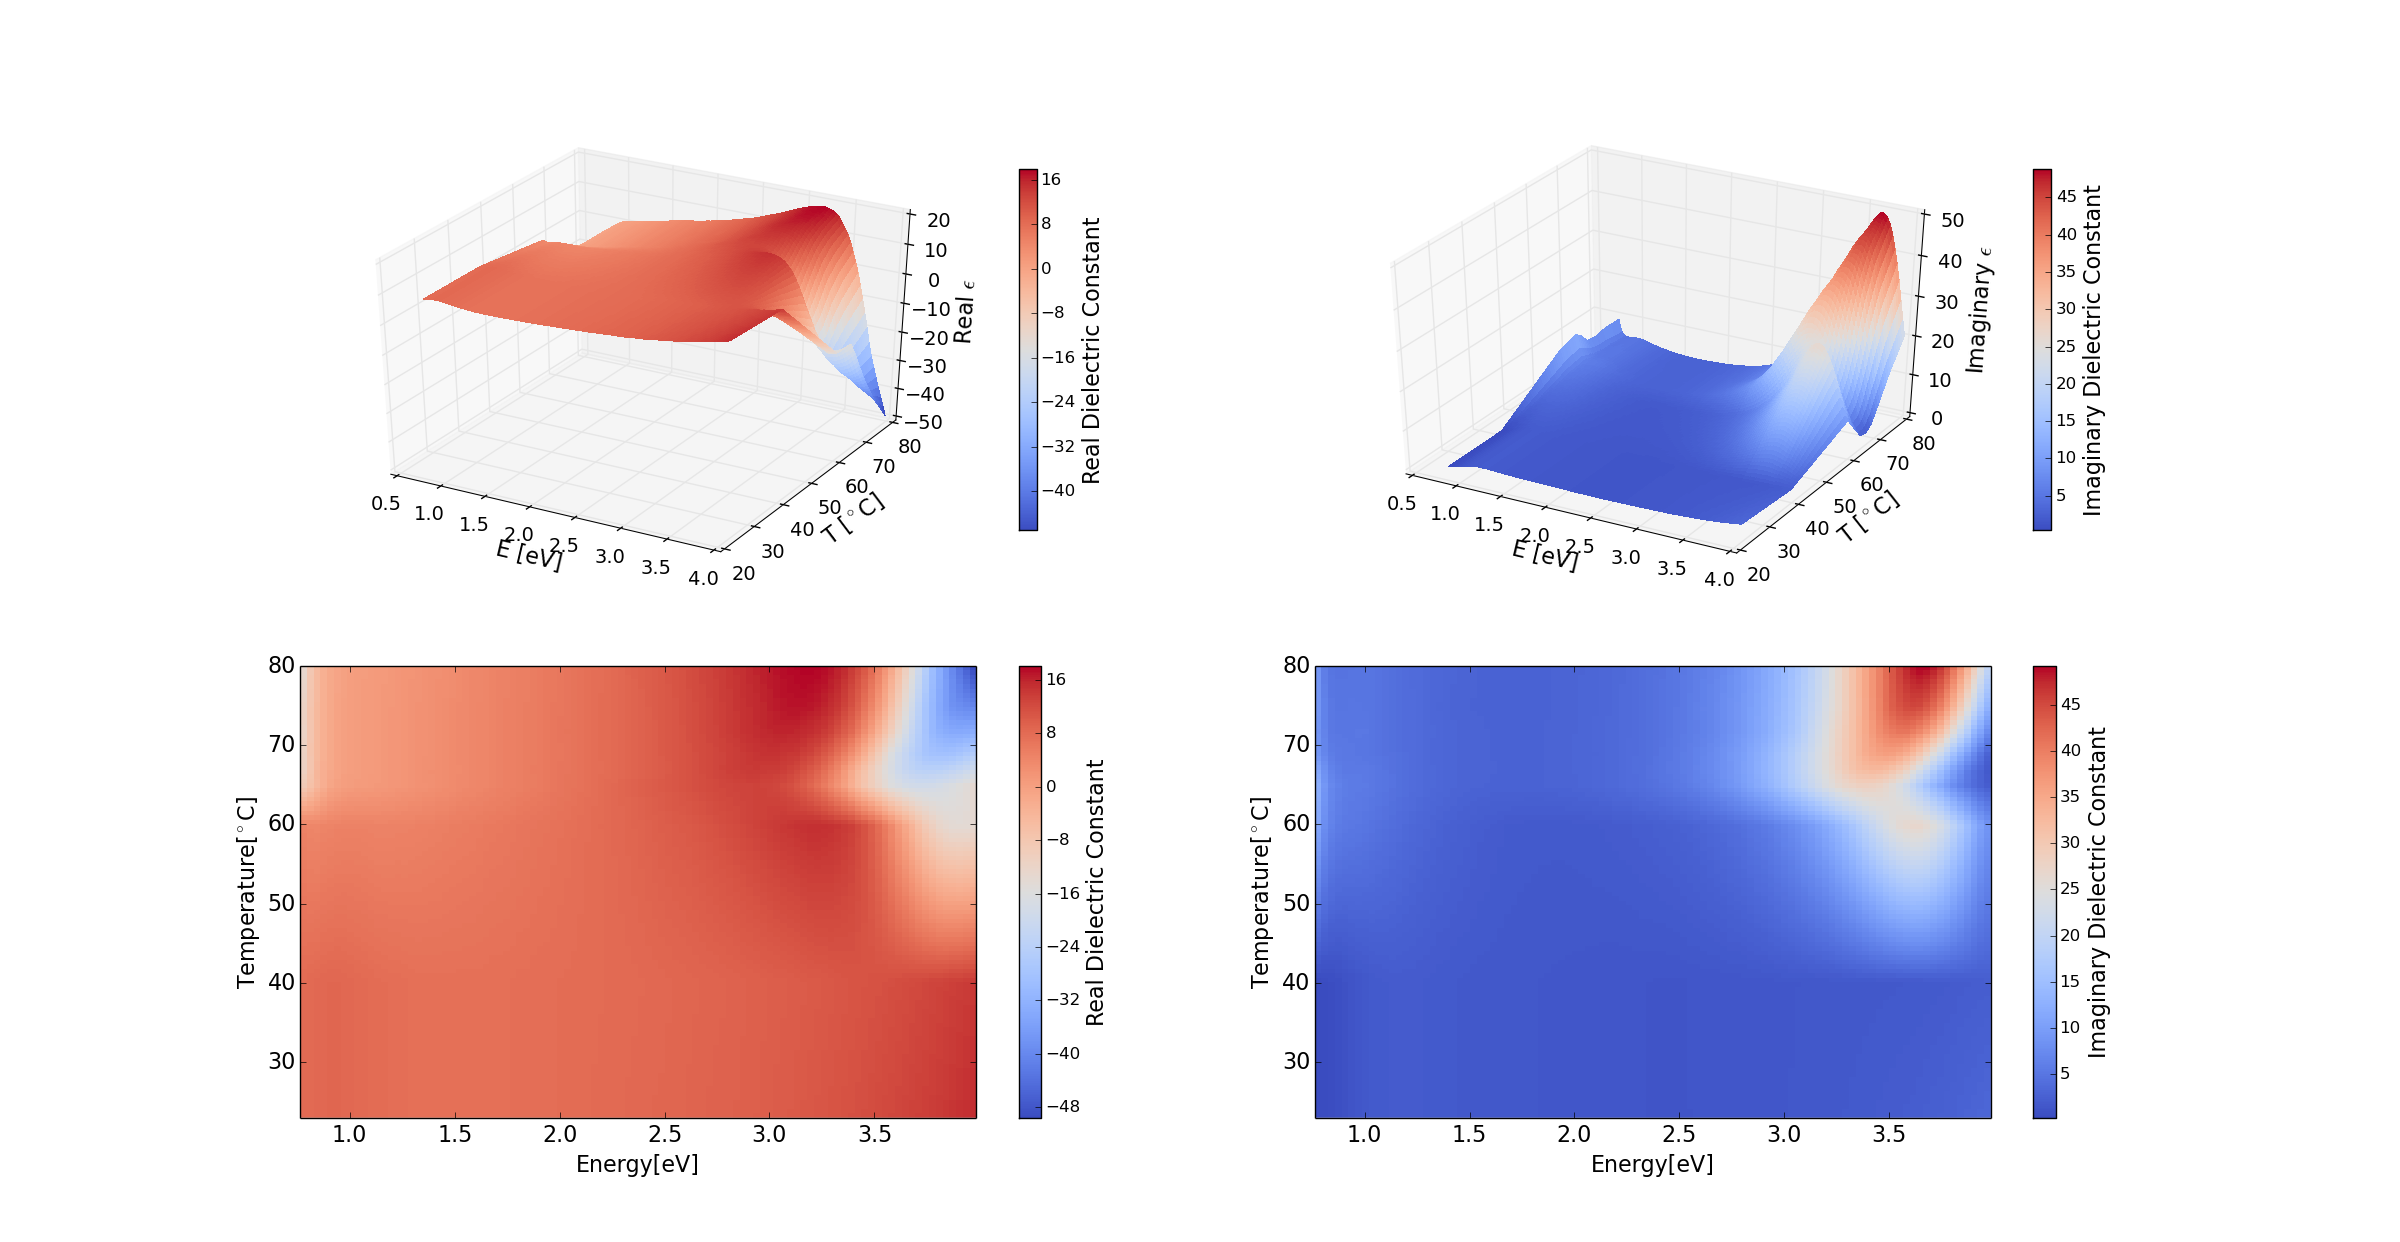
\includegraphics[width=\textwidth]{Results/interpPermittivity.png}
    \caption{Dielectric Function}
    \label{fig:DF}
\end{figure}
%

\section{Simulation results}
The following simulations are done with an incident plane wave of direction 
$(\theta_i,\phi_i) = (45^{\circ},0^{\circ})$, on VO$_2$ particles supported by a SiO$_2$ substrate
with truncation ratio $t_r = 0$. The surrounding medium is air with $\varepsilon(\omega,T) = 1$.
The particles are arranged in a square lattice with lattice constant $L = 45$nm and the
particle-particle interaction is given by a dipole contribution. The multipole truncation
is set to $M = 16$.


\subsection{Simulation 1; $R = 10$nm, p-polarized incident light}
%
\begin{figure}
    \centering
    \begin{subfigure}[b]{0.49\textwidth}
        \centering
        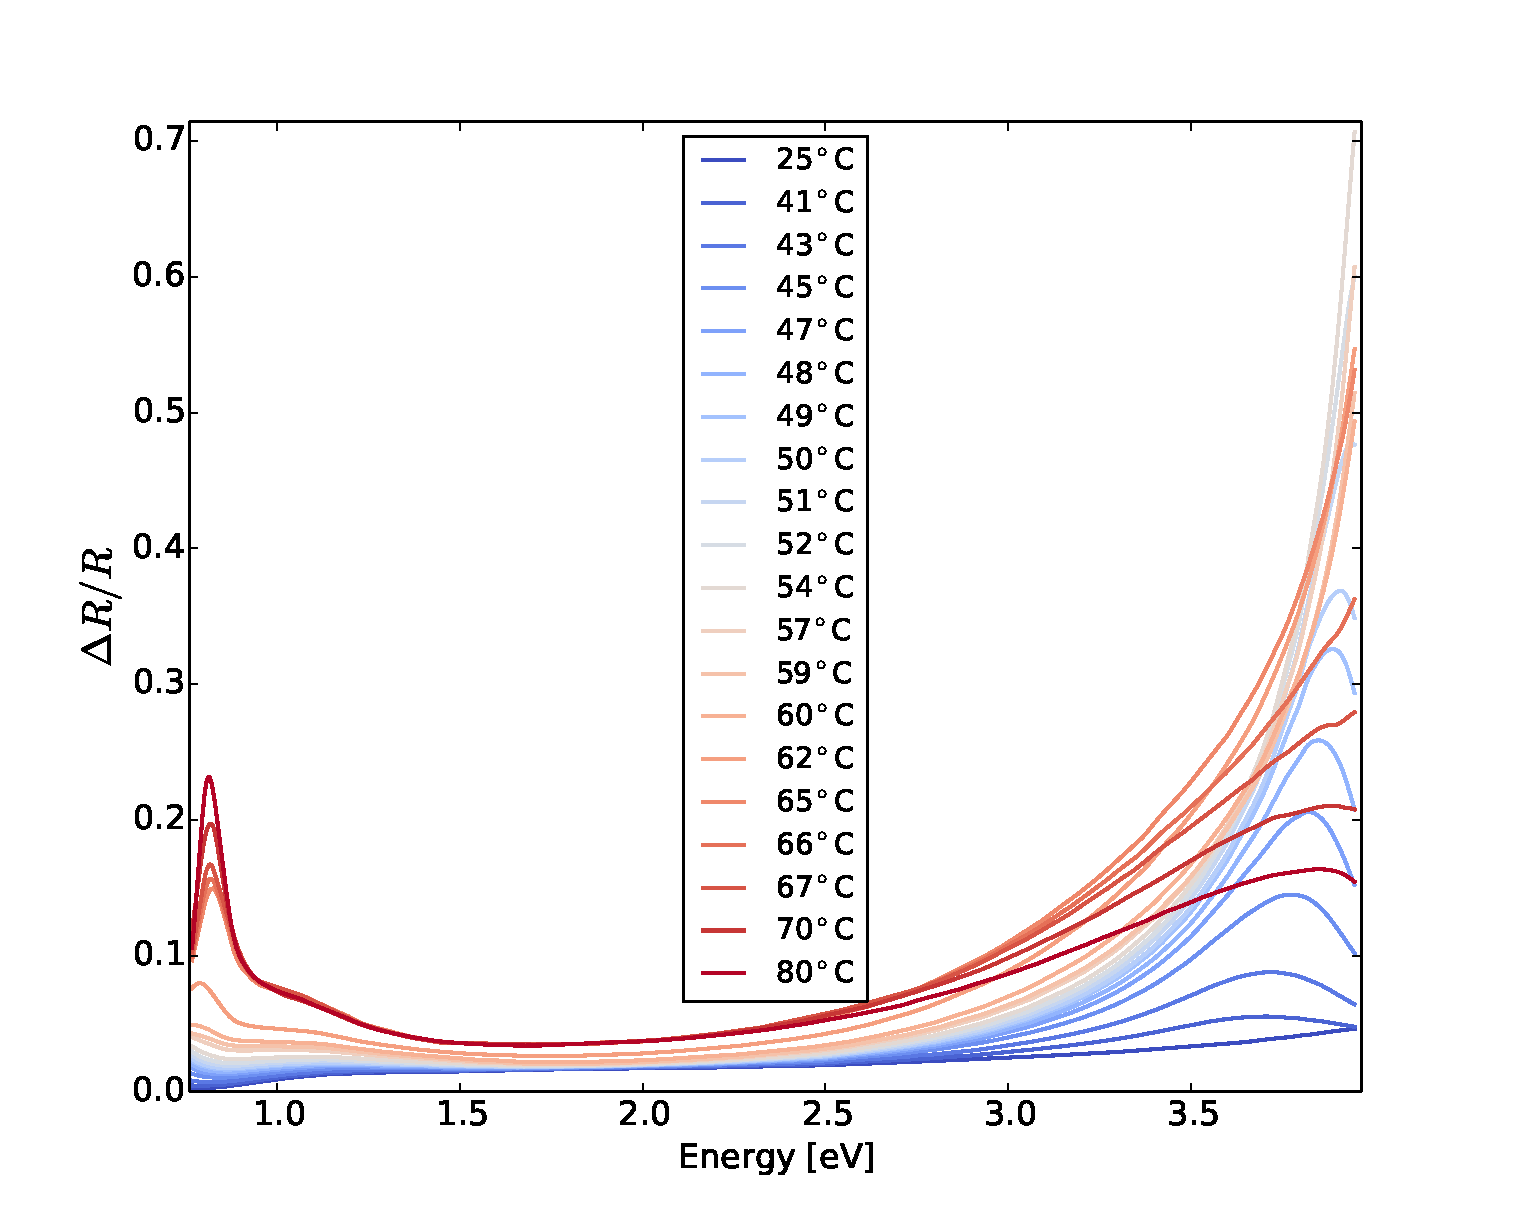
\includegraphics[width=\textwidth]{Results/Sim1/dR.pdf}
        \caption{}
        \label{fig:}
    \end{subfigure}
    %\hfill
    \begin{subfigure}[b]{0.49\textwidth}
        \centering
        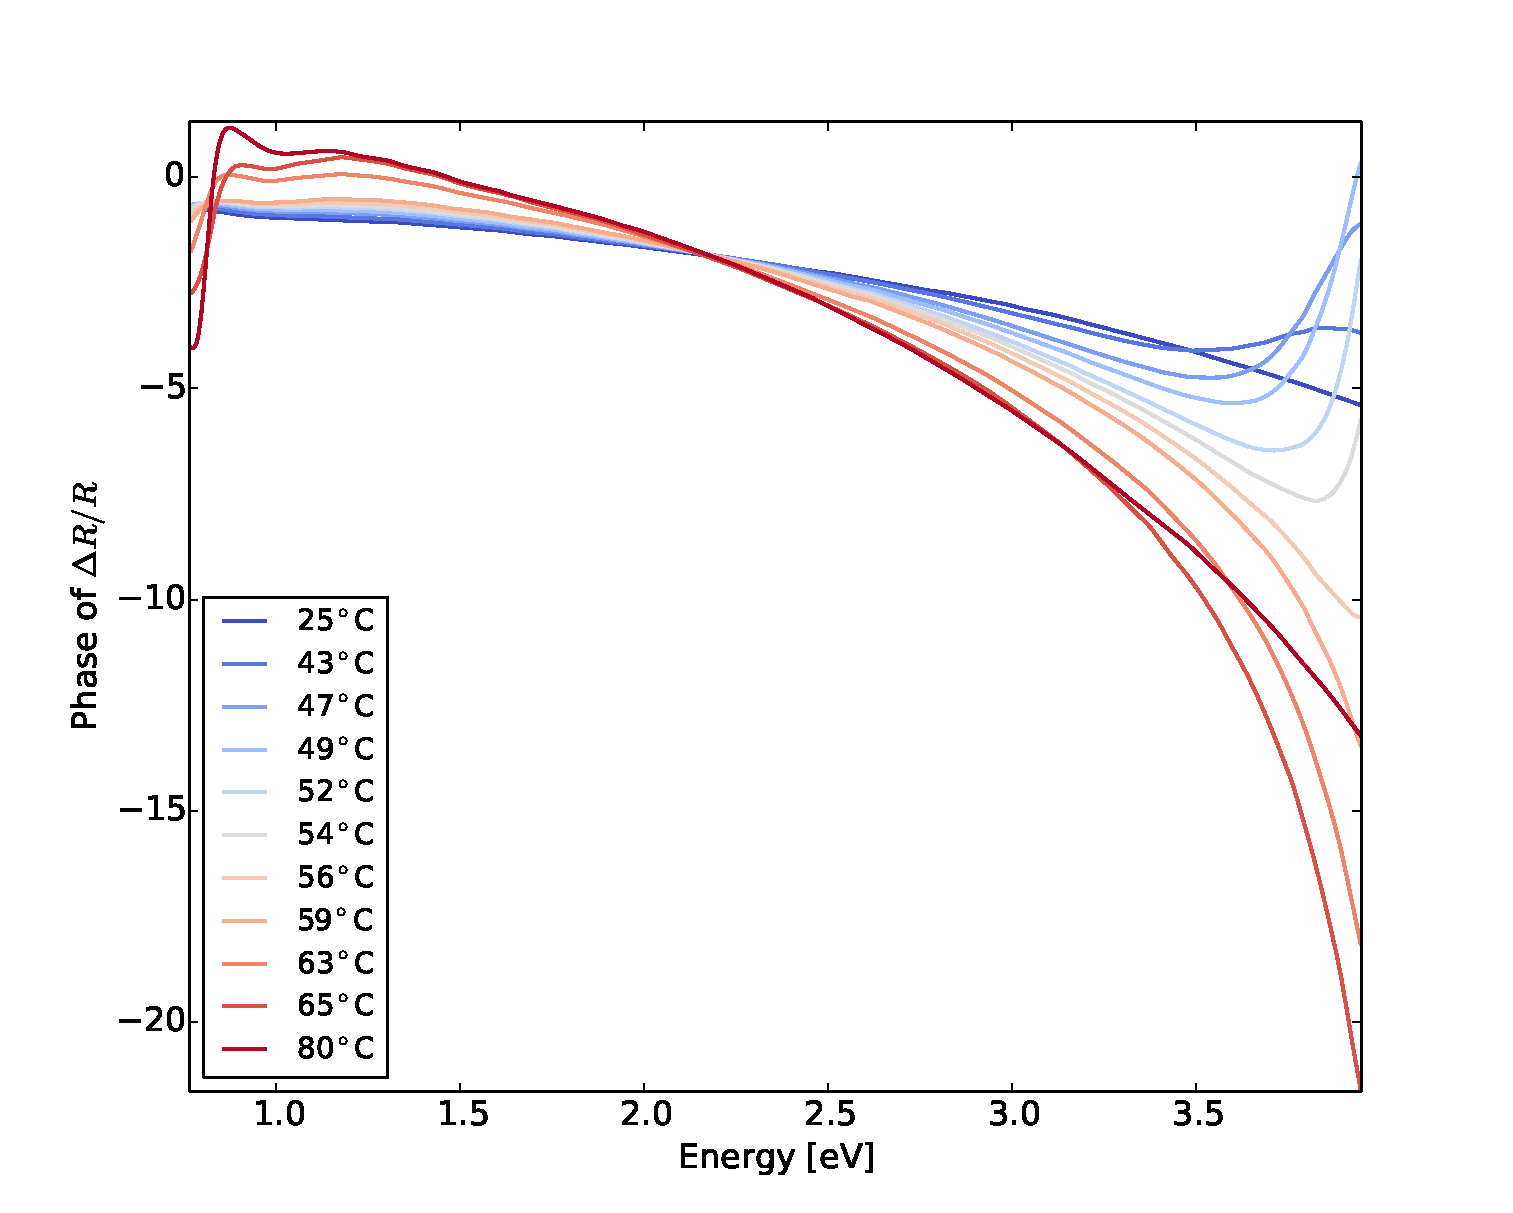
\includegraphics[width=\textwidth]{Results/Sim1/dRphase.pdf}
        \caption{}
        \label{fig:}
    \end{subfigure}
    \caption{Relative reflectance $\Delta R/R$}
    \label{fig:1}
\end{figure}
%
%
\begin{figure}
    \centering
    \begin{subfigure}[b]{0.49\textwidth}
        \centering
        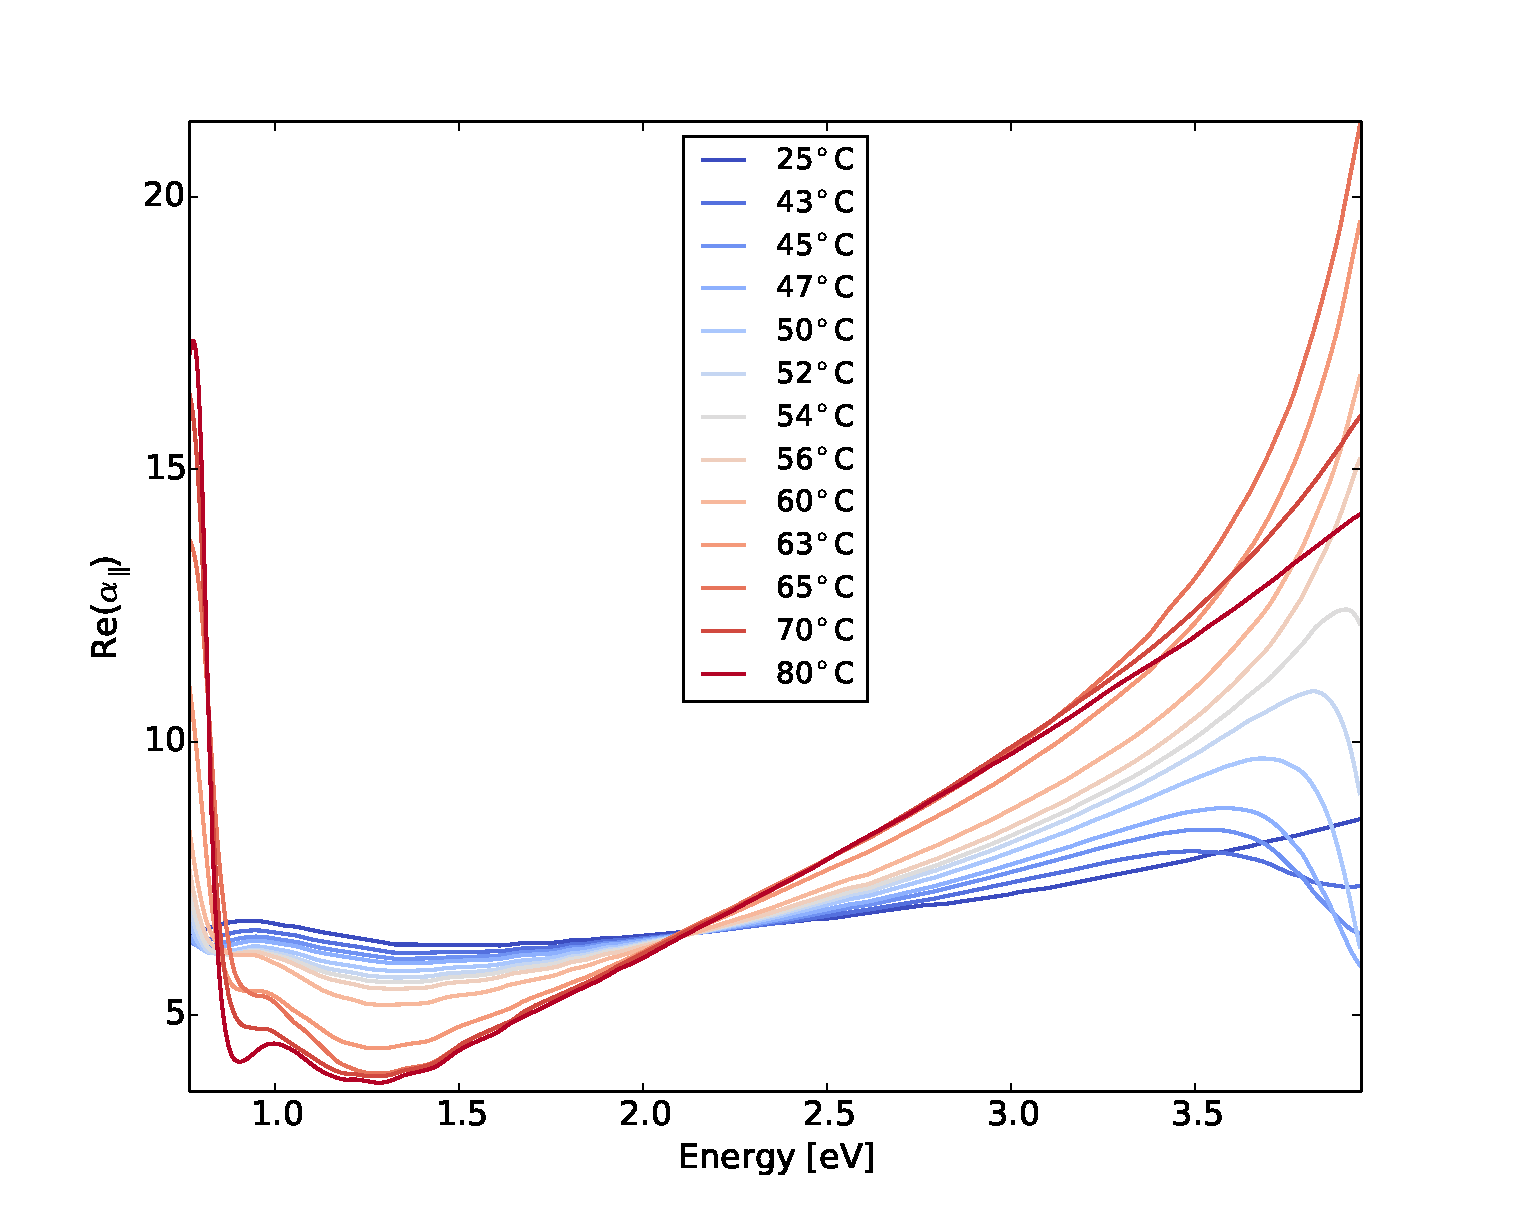
\includegraphics[width=\textwidth]{Results/Sim1/re_alpha_parallel.pdf}
        \caption{}
        \label{fig:2}
    \end{subfigure}
    %\hfill
    \begin{subfigure}[b]{0.49\textwidth}
        \centering
        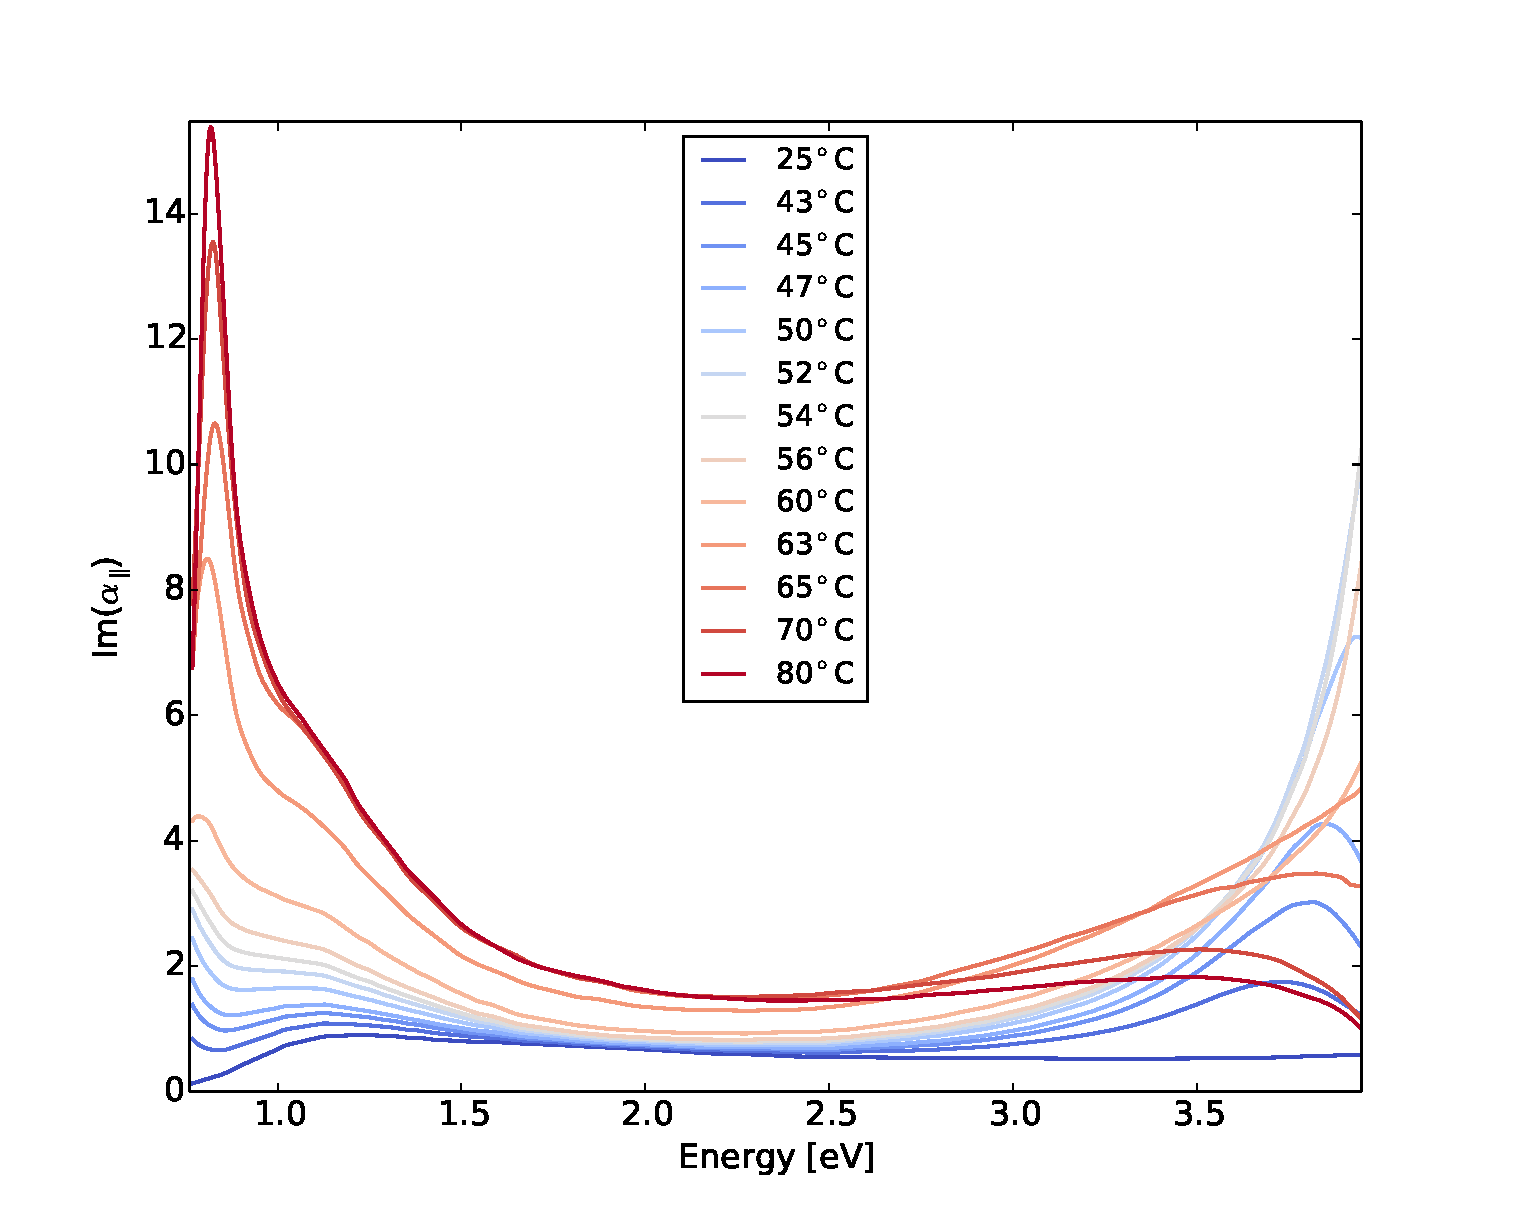
\includegraphics[width=\textwidth]{Results/Sim1/im_alpha_parallel.pdf}
        \caption{}
        \label{fig:2}
    \end{subfigure}
    %\hfill
    \begin{subfigure}[b]{0.49\textwidth}
        \centering
        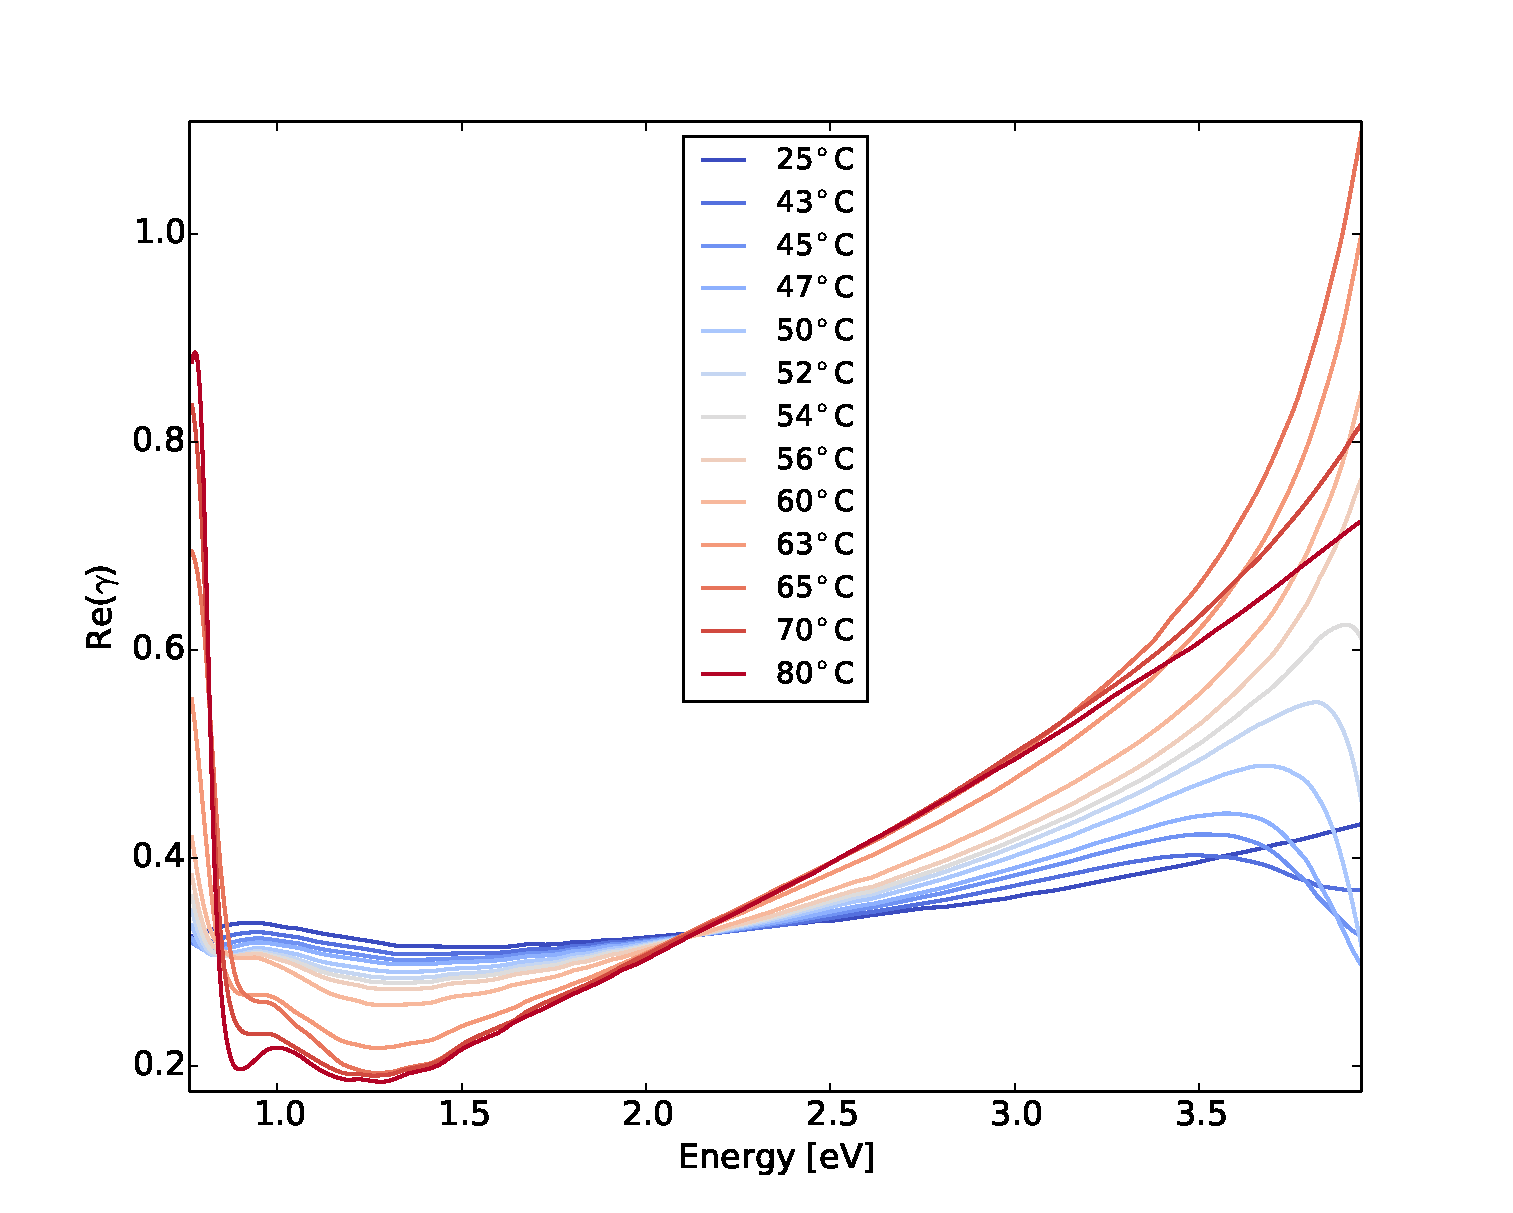
\includegraphics[width=\textwidth]{Results/Sim1/re_gamma.pdf}
        \caption{}
        \label{fig:2}
    \end{subfigure}
    %\hfill
    \begin{subfigure}[b]{0.49\textwidth}
        \centering
        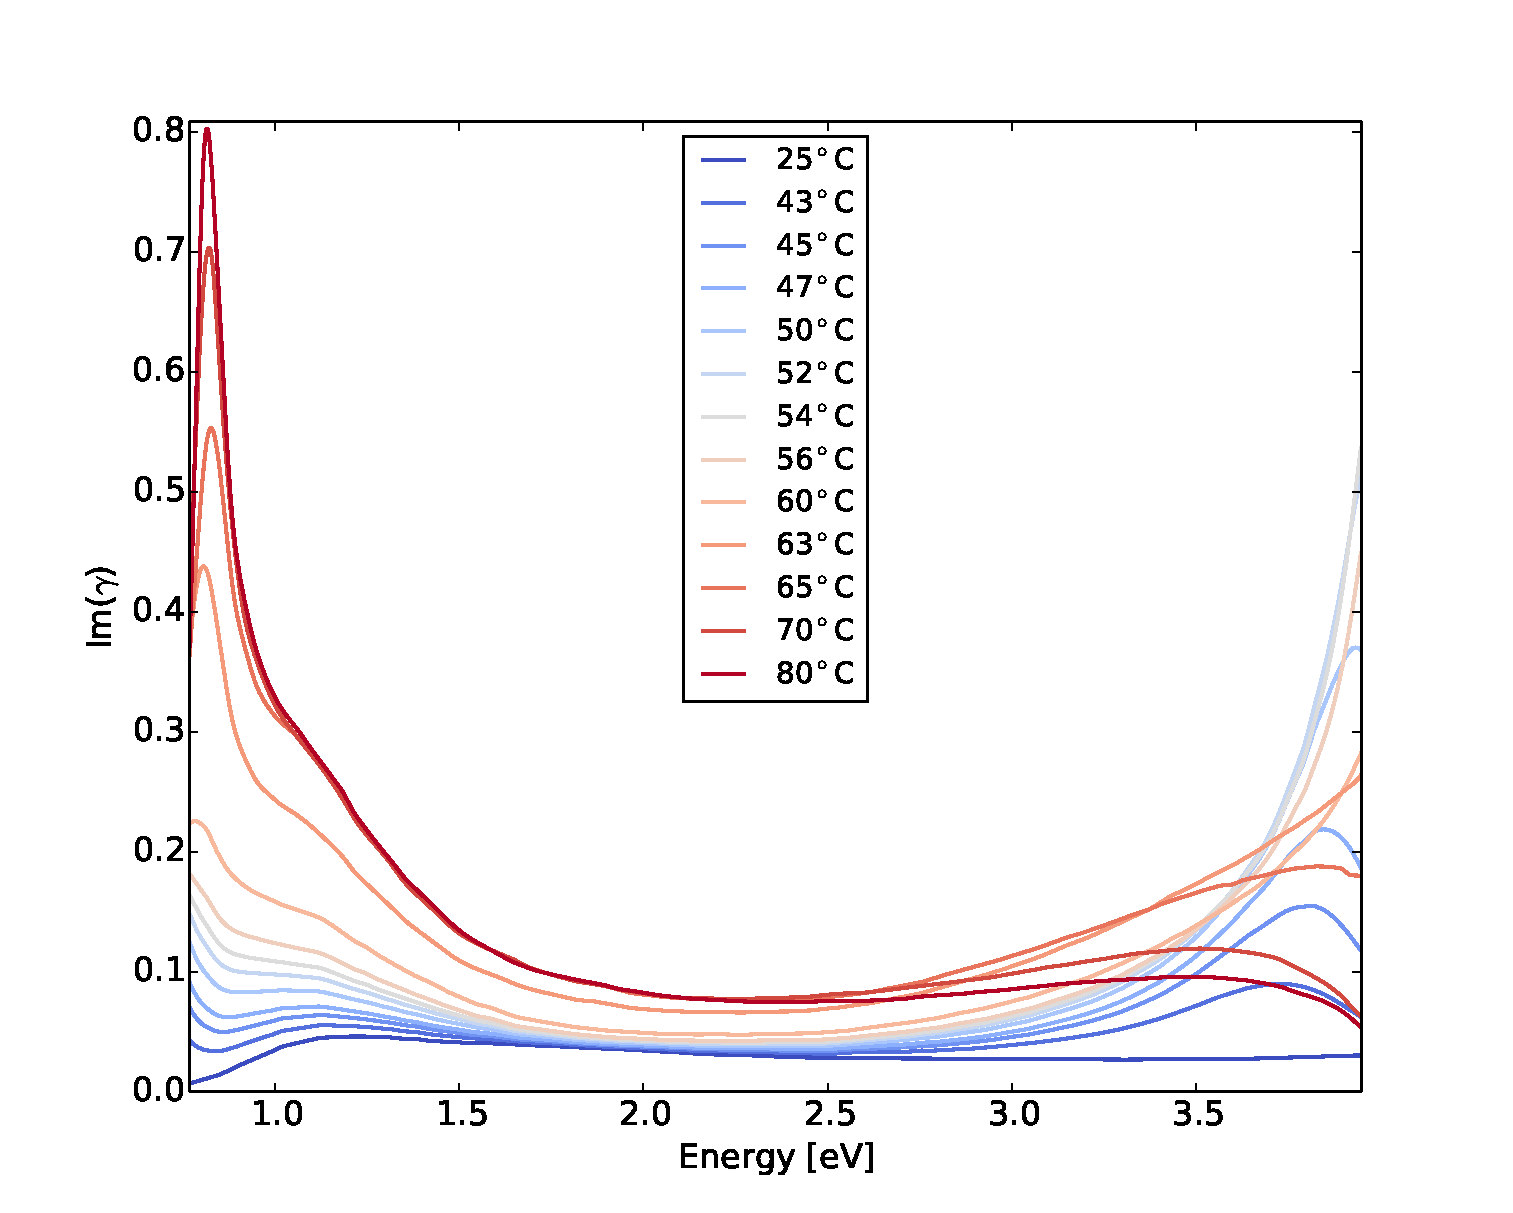
\includegraphics[width=\textwidth]{Results/Sim1/im_gamma.pdf}
        \caption{}
        \label{fig:2}
    \end{subfigure}
    \caption{Relative reflectance $\Delta R/R$}
    \label{fig:}
\end{figure}
%
%
\begin{figure}
    \centering
    \begin{subfigure}[b]{0.49\textwidth}
        \centering
        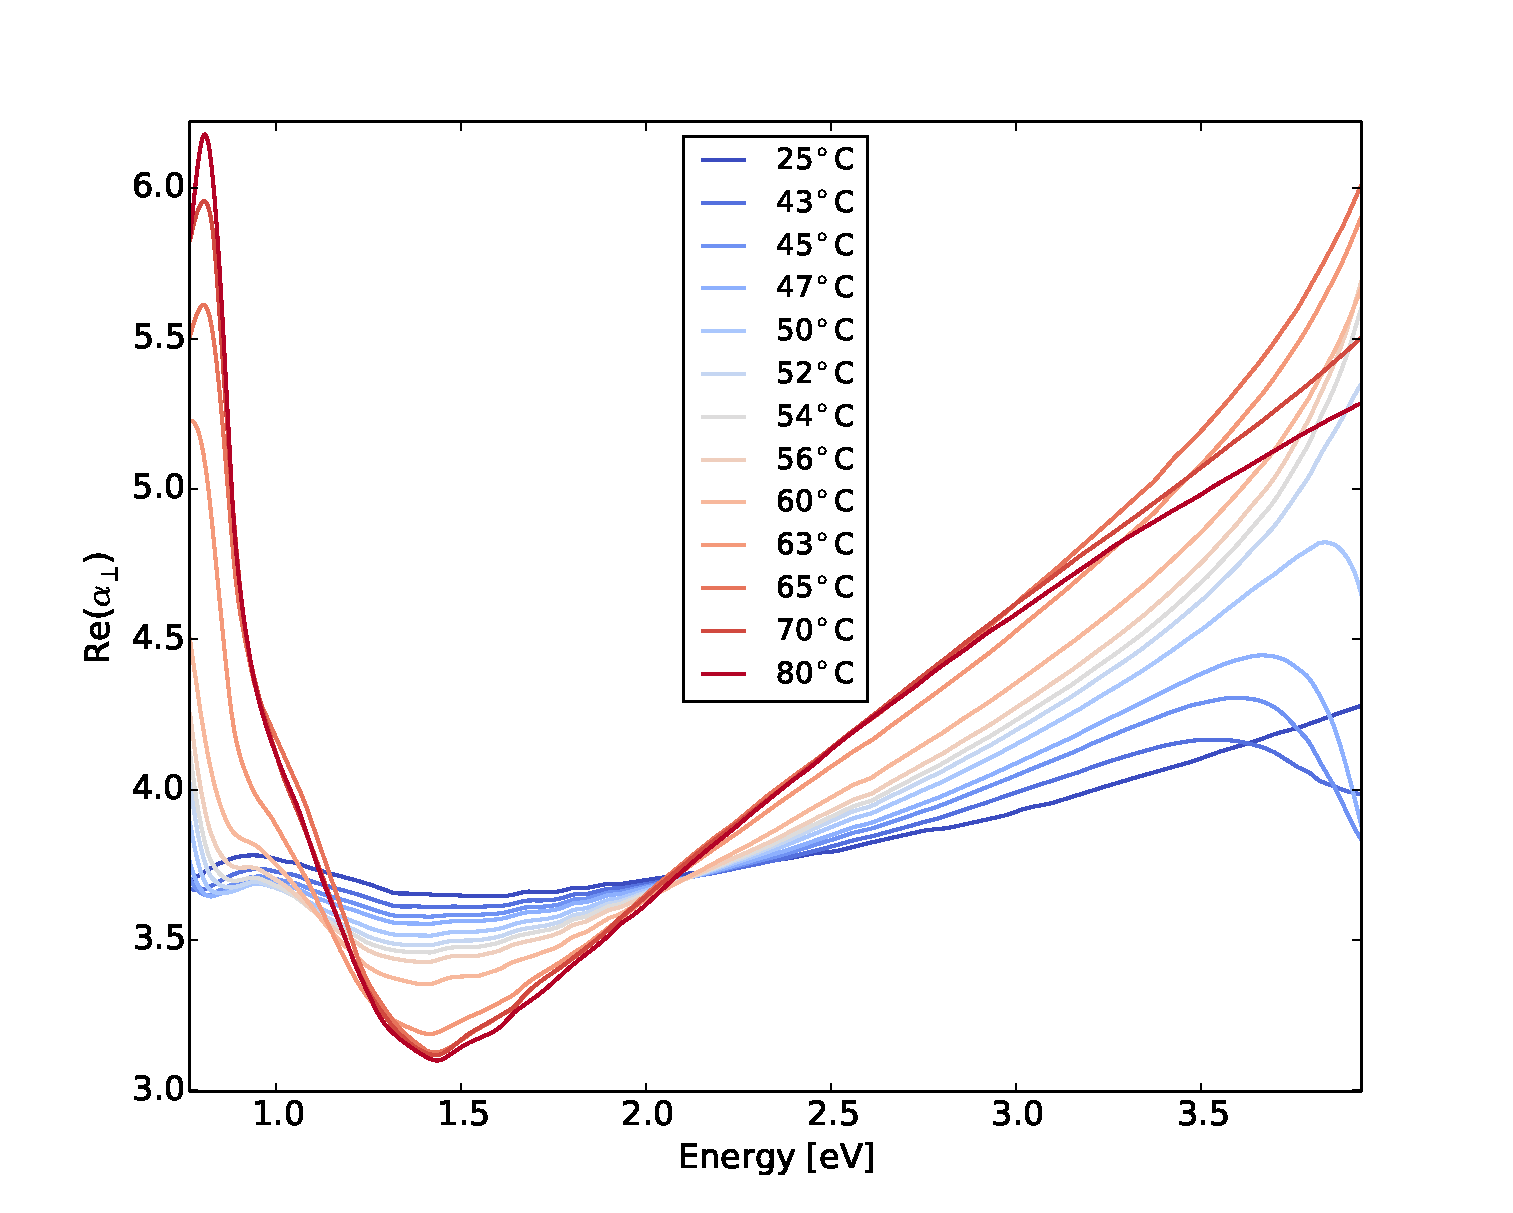
\includegraphics[width=\textwidth]{Results/Sim1/re_alpha_perp.pdf}
        \caption{}
        \label{fig:}
    \end{subfigure}
    %\hfill
    \begin{subfigure}[b]{0.49\textwidth}
        \centering
        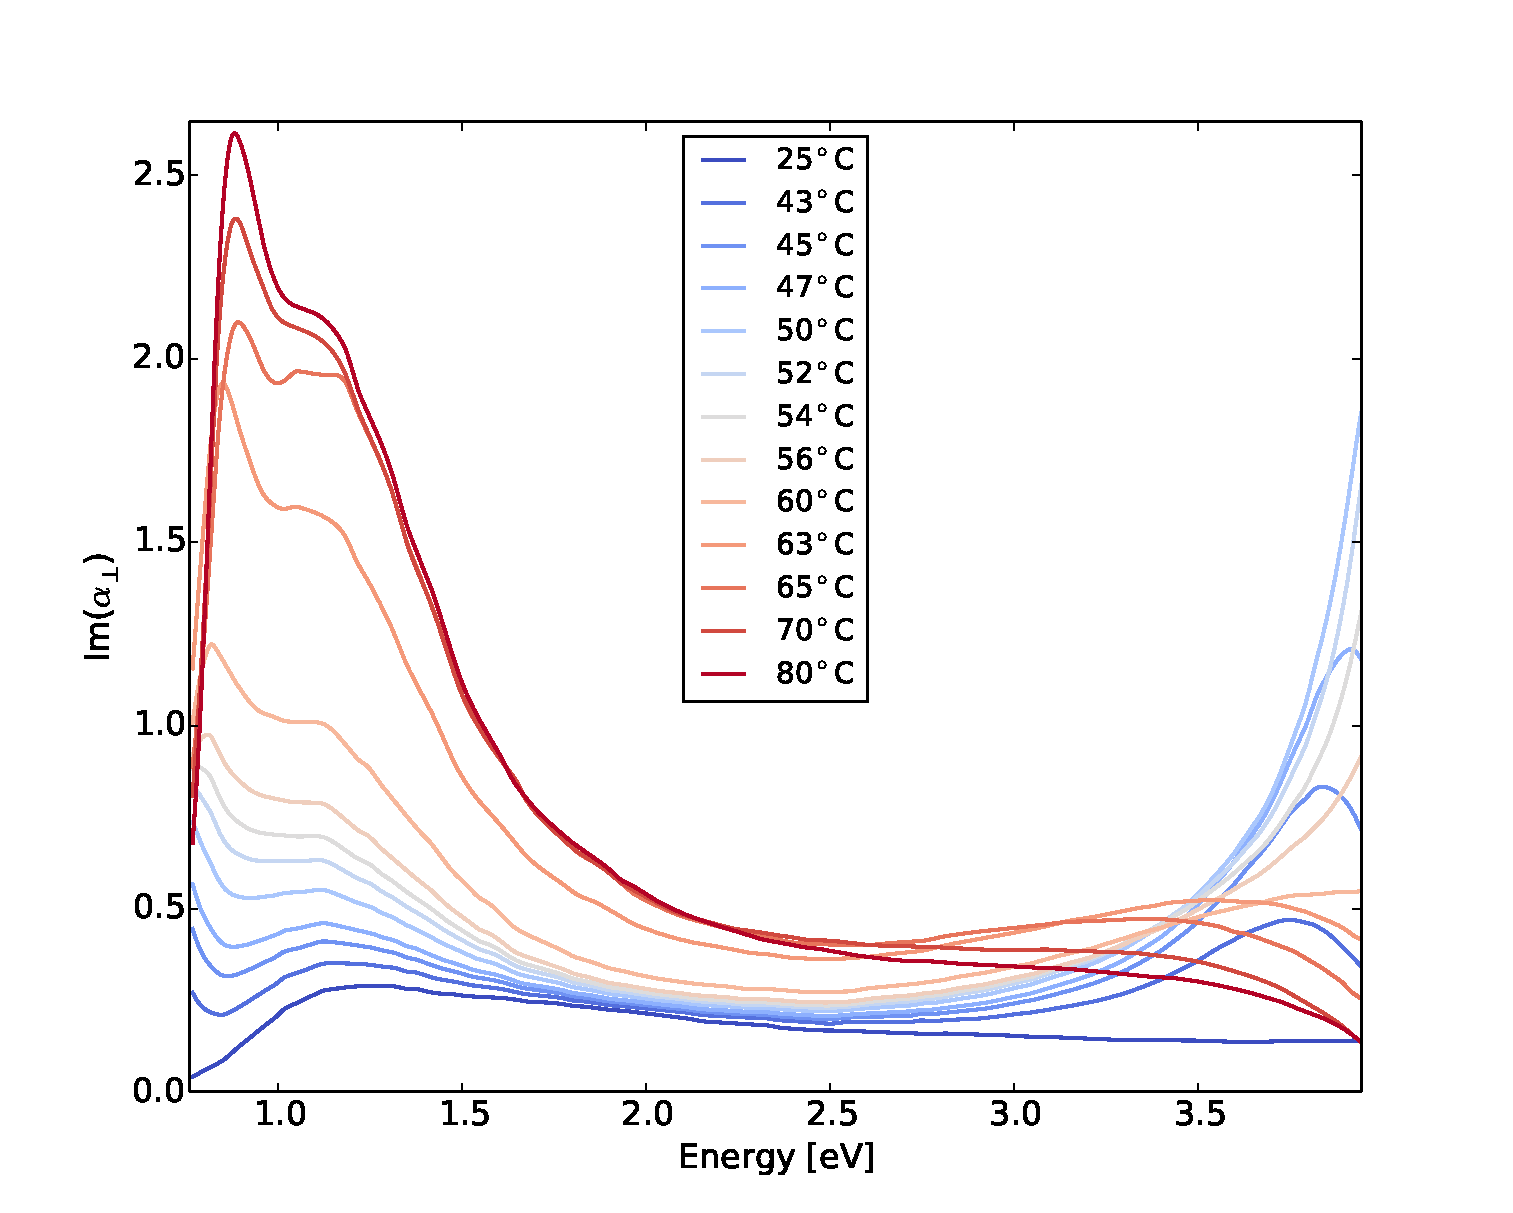
\includegraphics[width=\textwidth]{Results/Sim1/im_alpha_perp.pdf}
        \caption{}
        \label{fig:}
    \end{subfigure}
    %\hfill
    \begin{subfigure}[b]{0.49\textwidth}
        \centering
        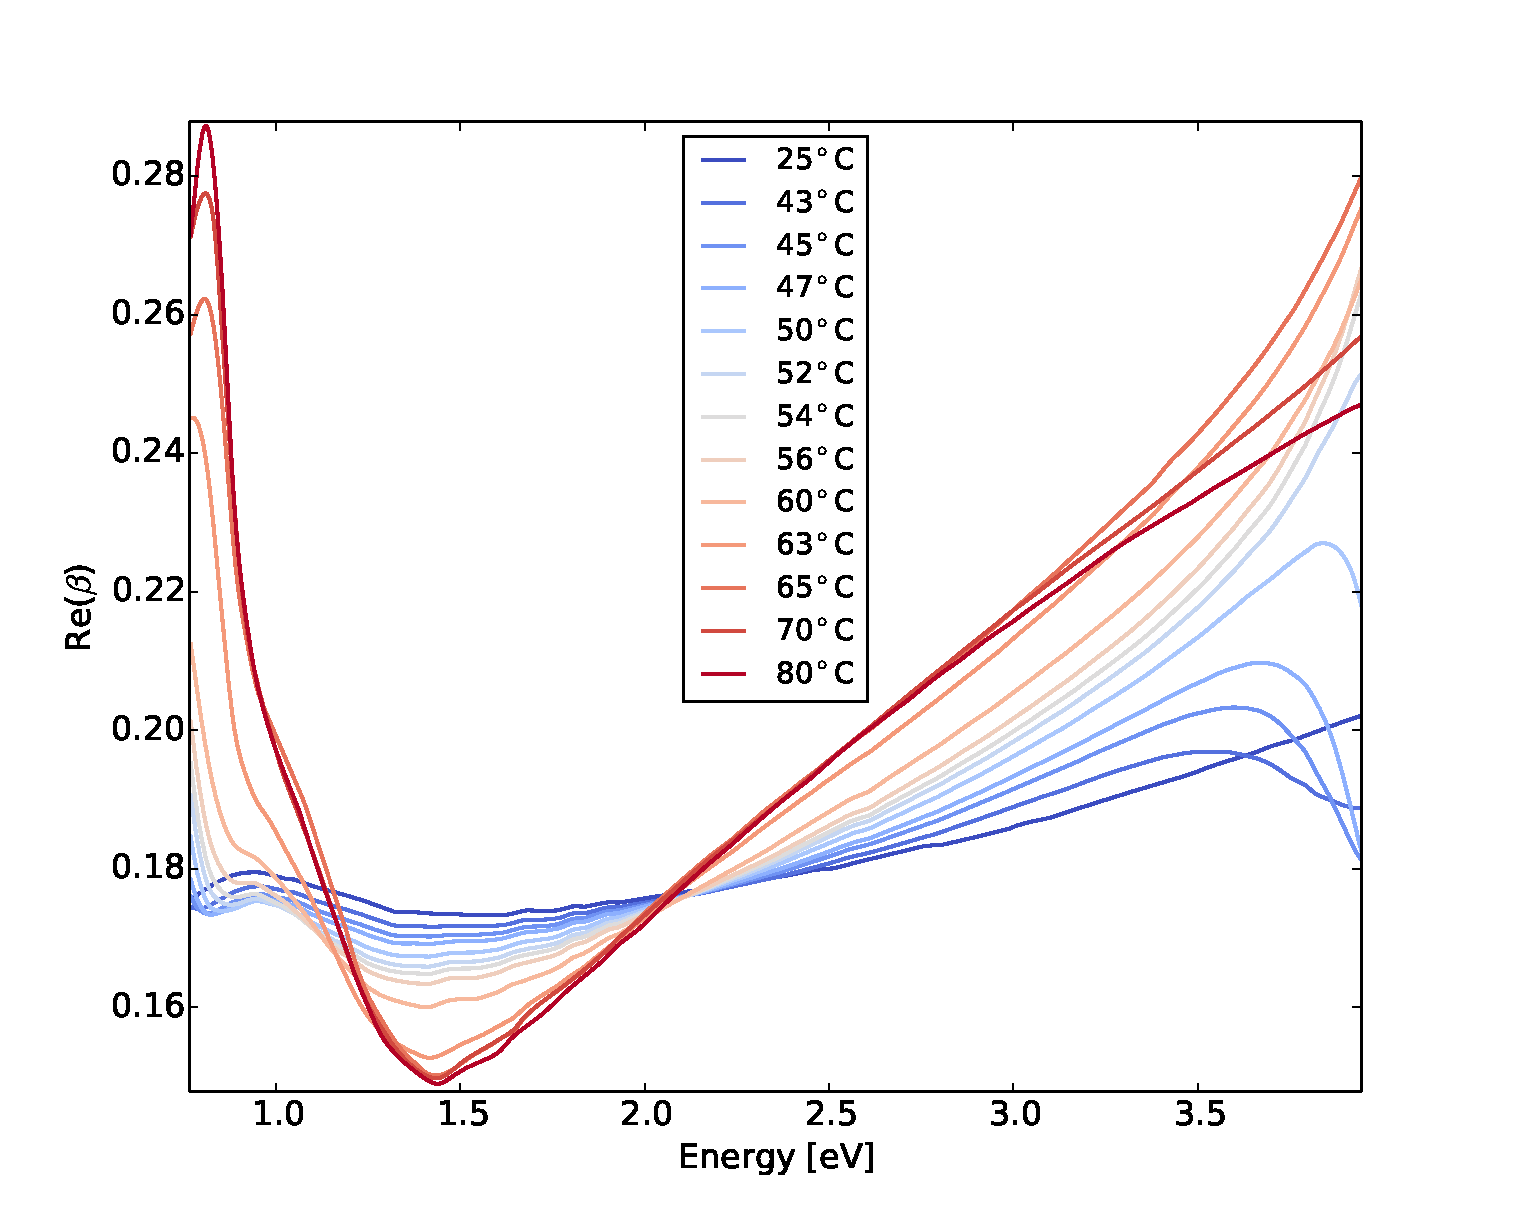
\includegraphics[width=\textwidth]{Results/Sim1/re_beta.pdf}
        \caption{}
        \label{fig:2}
    \end{subfigure}
    %\hfill
    \begin{subfigure}[b]{0.49\textwidth}
        \centering
        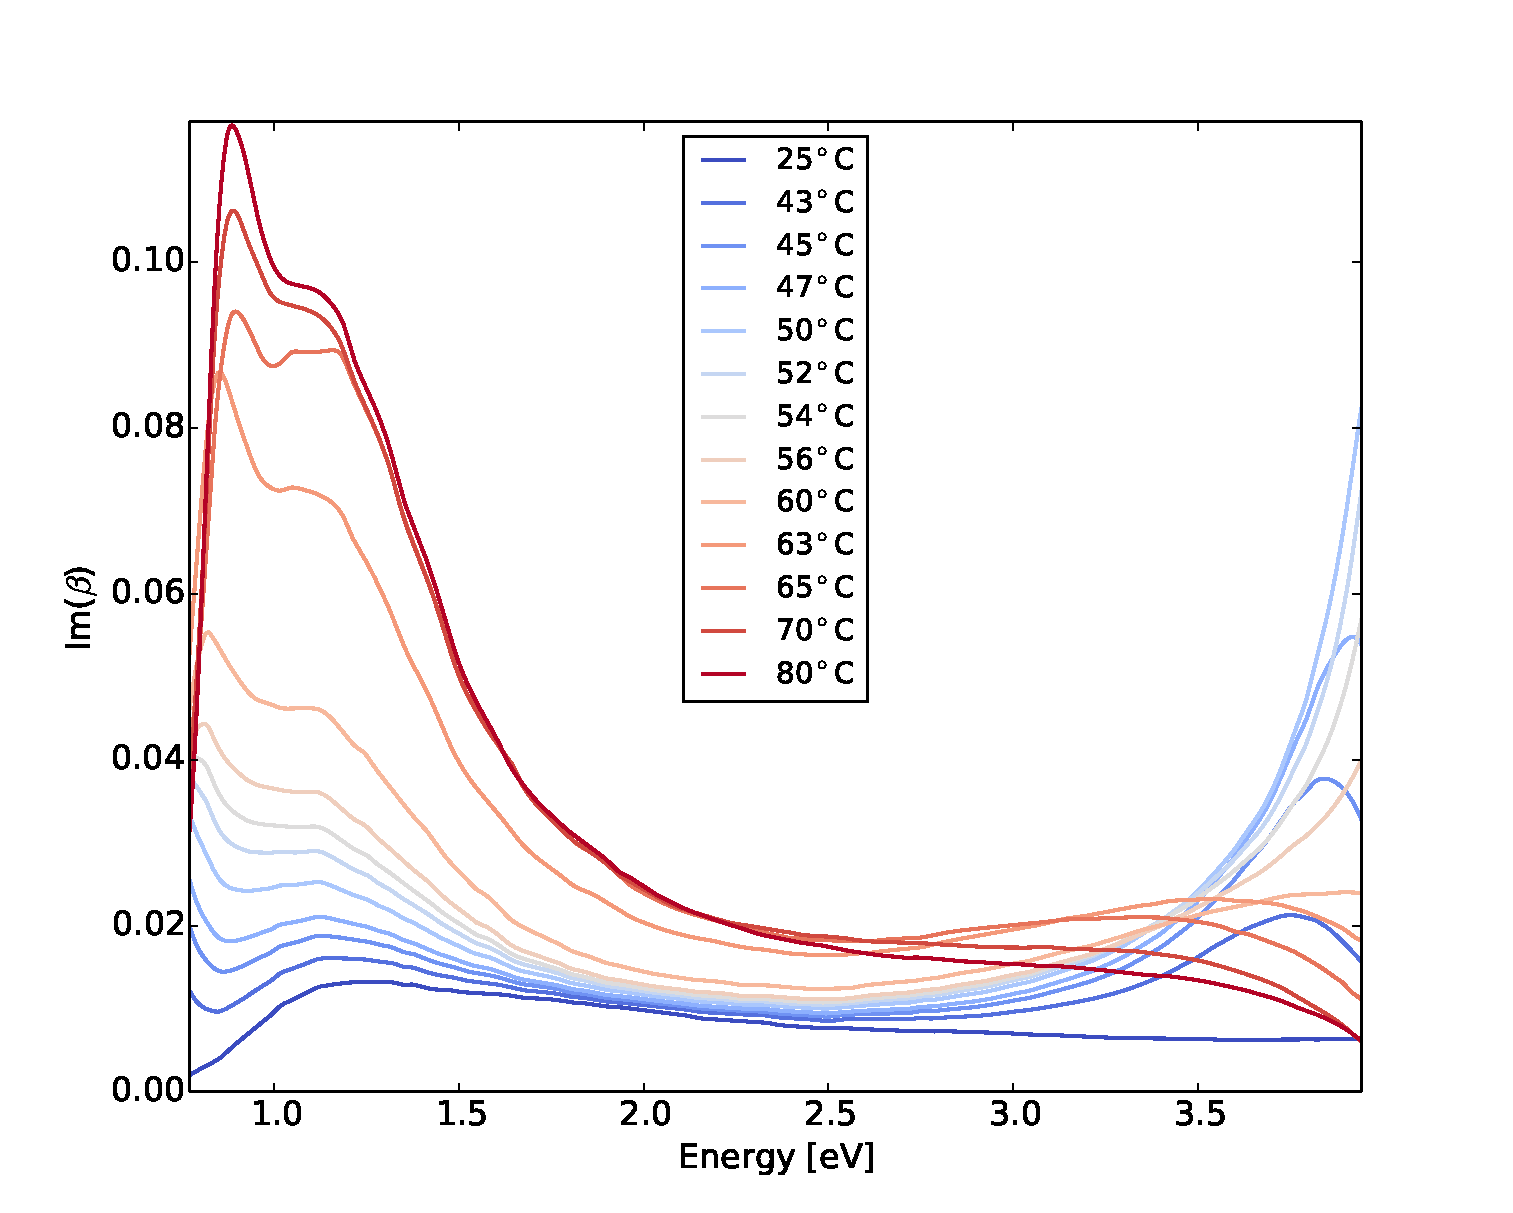
\includegraphics[width=\textwidth]{Results/Sim1/im_beta.pdf}
        \caption{}
        \label{fig:2}
    \end{subfigure}
    \caption{Relative reflectance $\Delta R/R$}
    \label{fig:}
\end{figure}
%


\subsection{Simulation 2; $R = 10$nm, s-polarized incident light}
%
\begin{figure}
    \centering
    \begin{subfigure}[b]{0.49\textwidth}
        \centering
        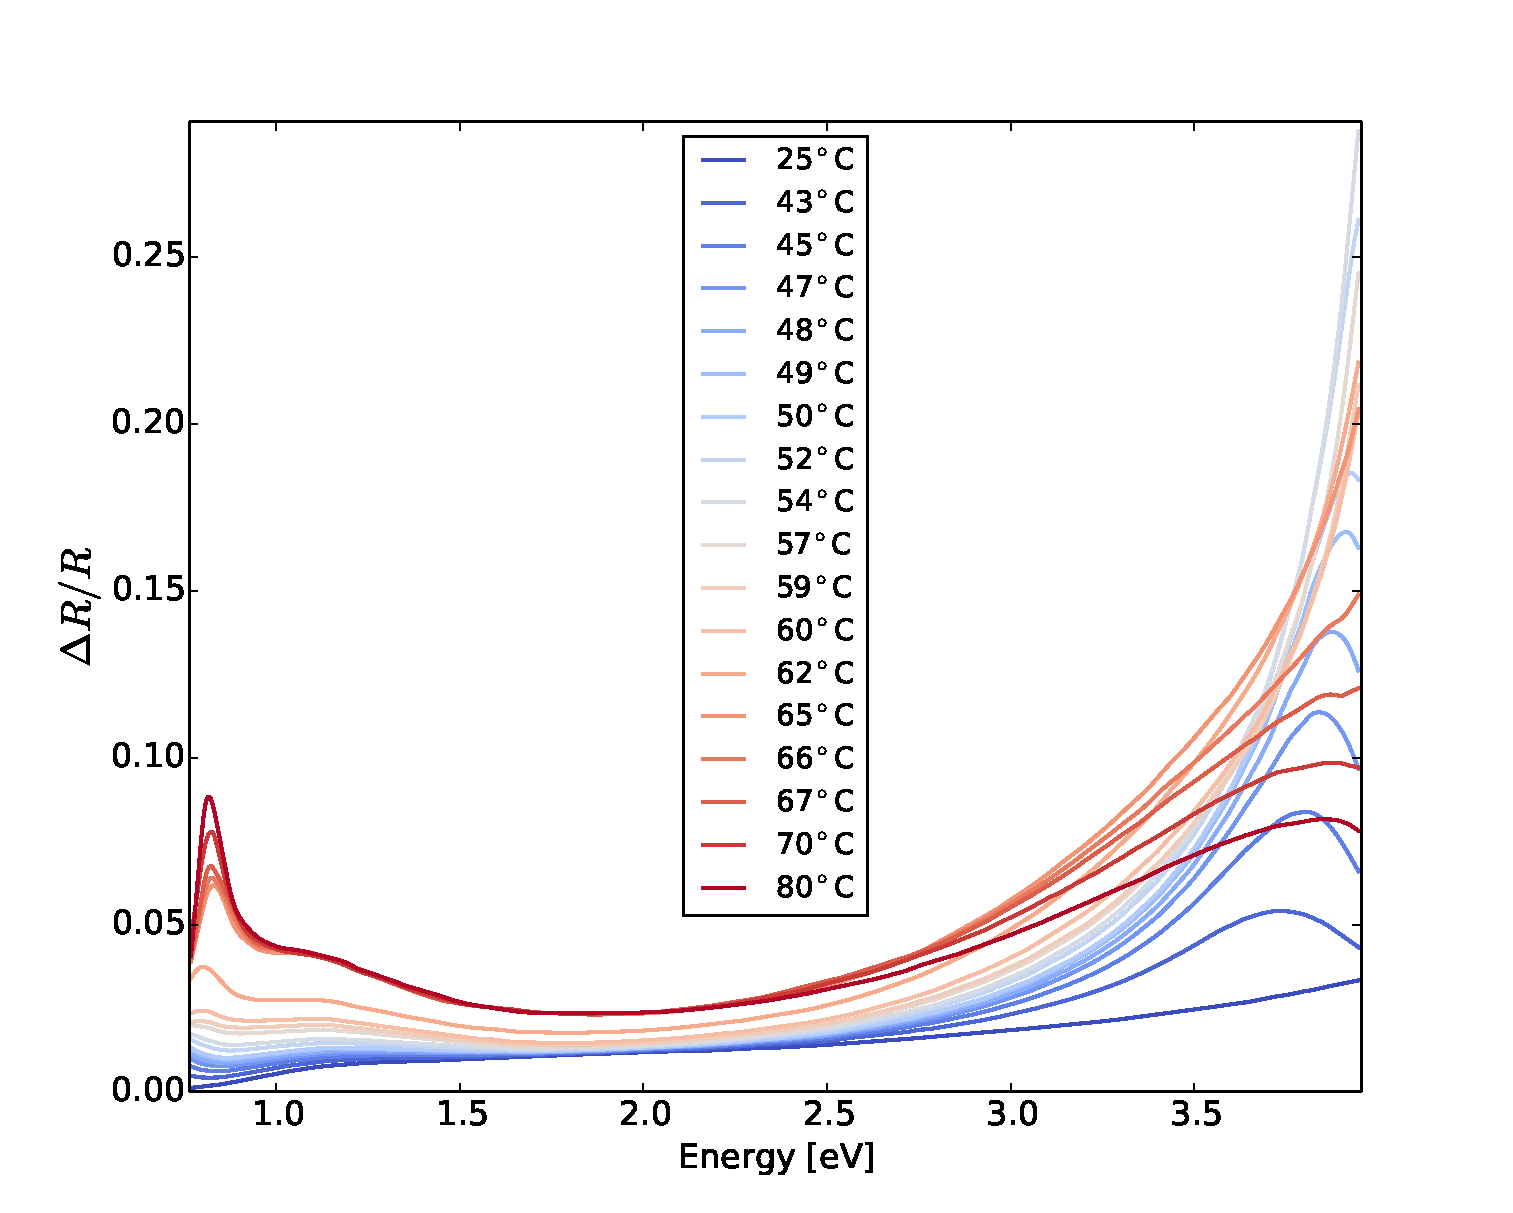
\includegraphics[width=\textwidth]{Results/Sim2/dR.pdf}h
        \caption{}
        \label{fig:}
    \end{subfigure}
    %\hfill
    \begin{subfigure}[b]{0.49\textwidth}
        \centering
        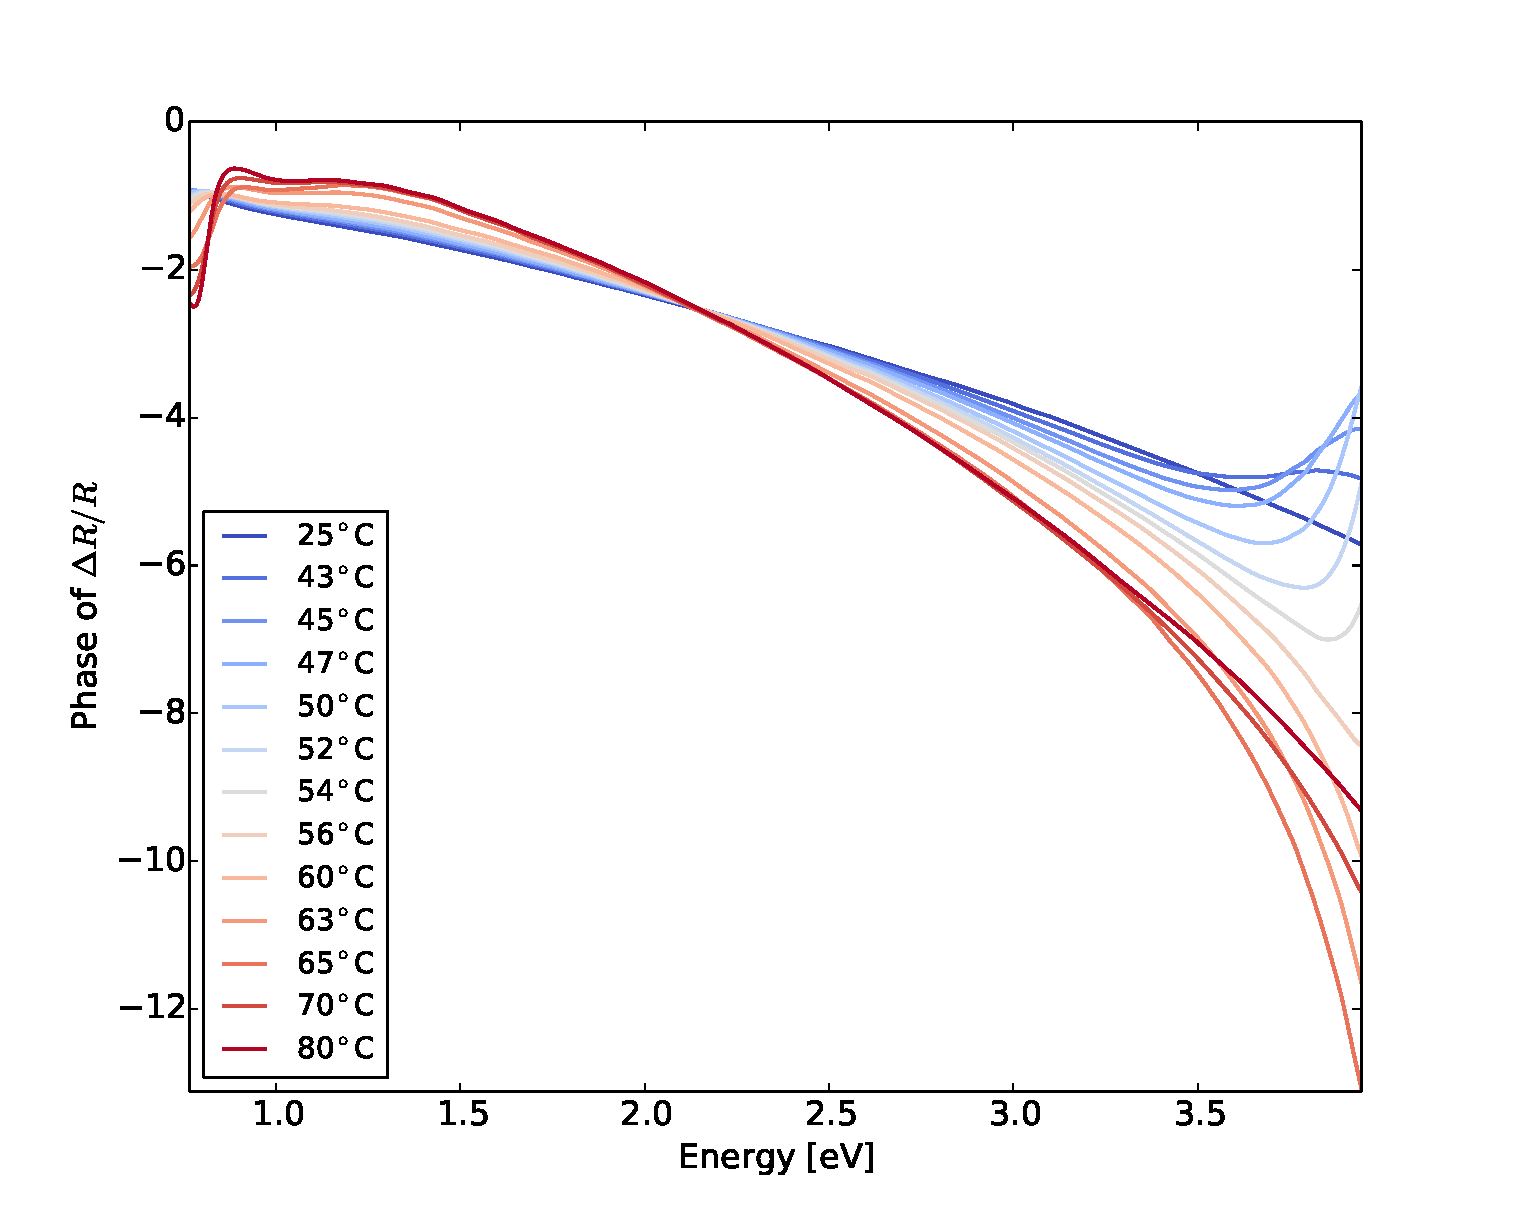
\includegraphics[width=\textwidth]{Results/Sim2/dRphase.pdf}
        \caption{}
        \label{fig:}
    \end{subfigure}
    \caption{Relative reflectance $\Delta R/R$}
    \label{fig:1}
\end{figure}
%
%
\begin{figure}
    \centering
    \begin{subfigure}[b]{0.49\textwidth}
        \centering
        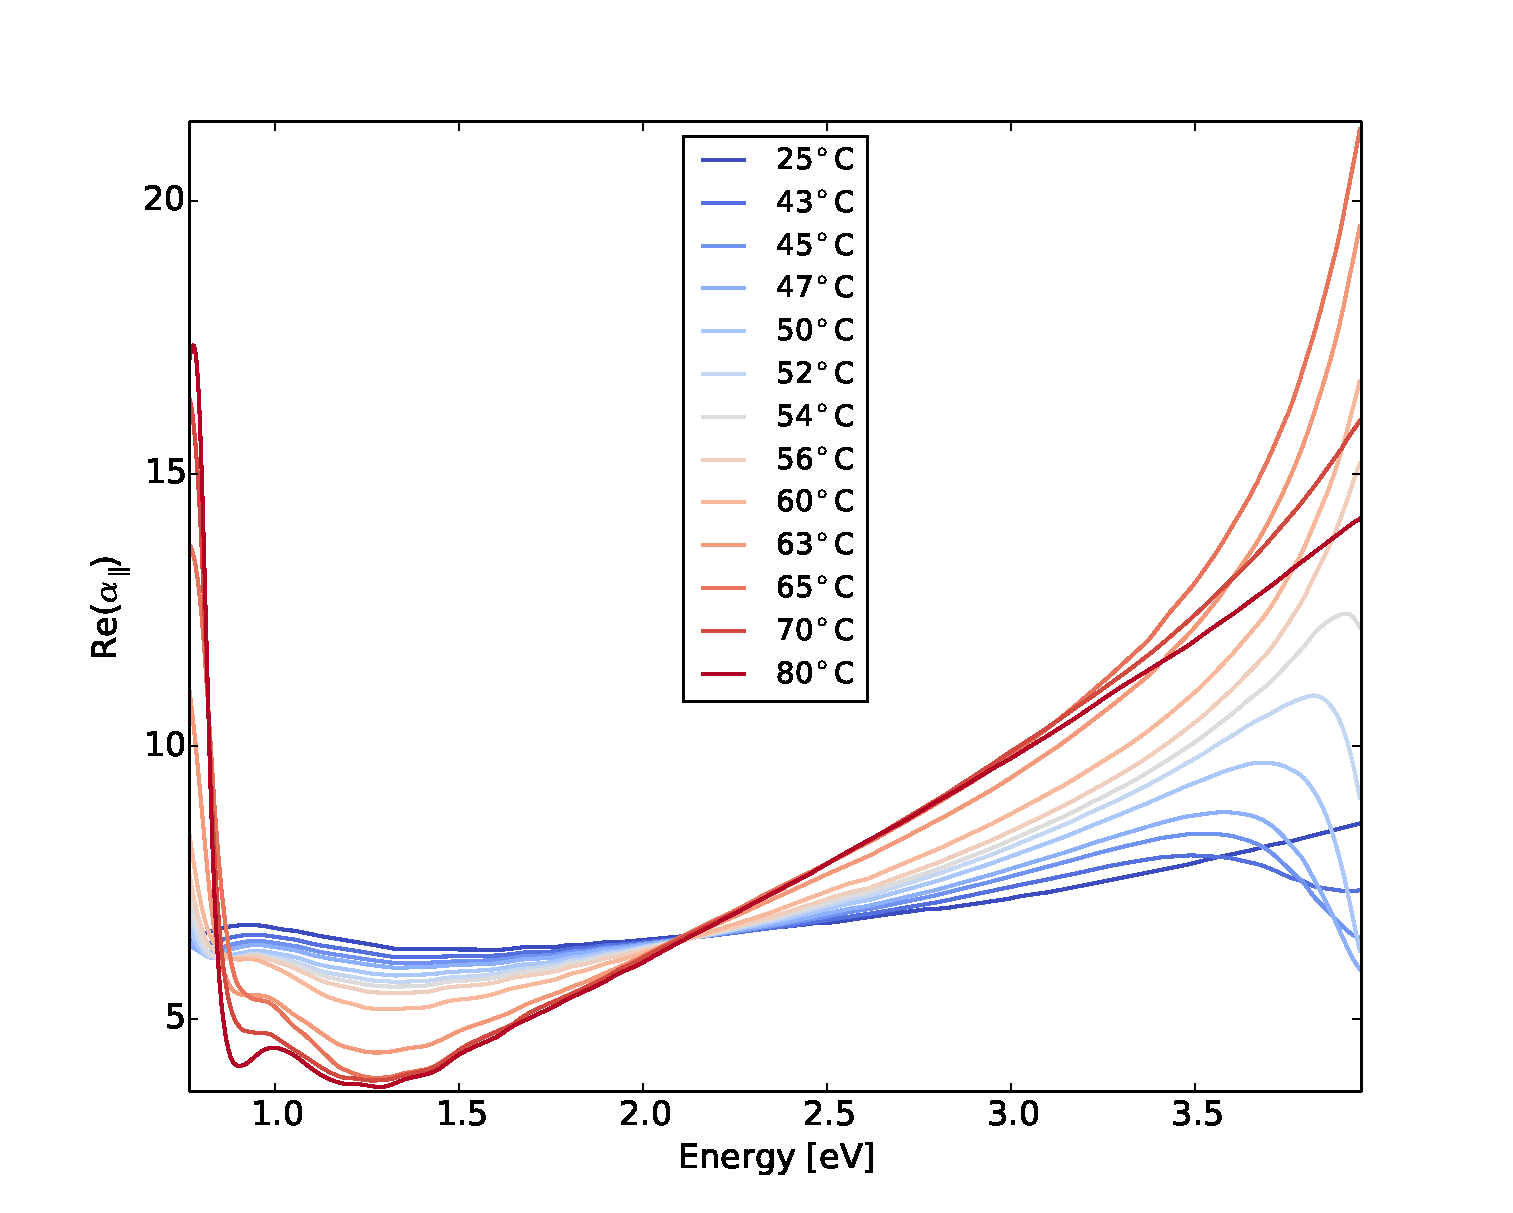
\includegraphics[width=\textwidth]{Results/Sim2/re_alpha_parallel.pdf}
        \caption{}
        \label{fig:2}
    \end{subfigure}
    %\hfill
    \begin{subfigure}[b]{0.49\textwidth}
        \centering
        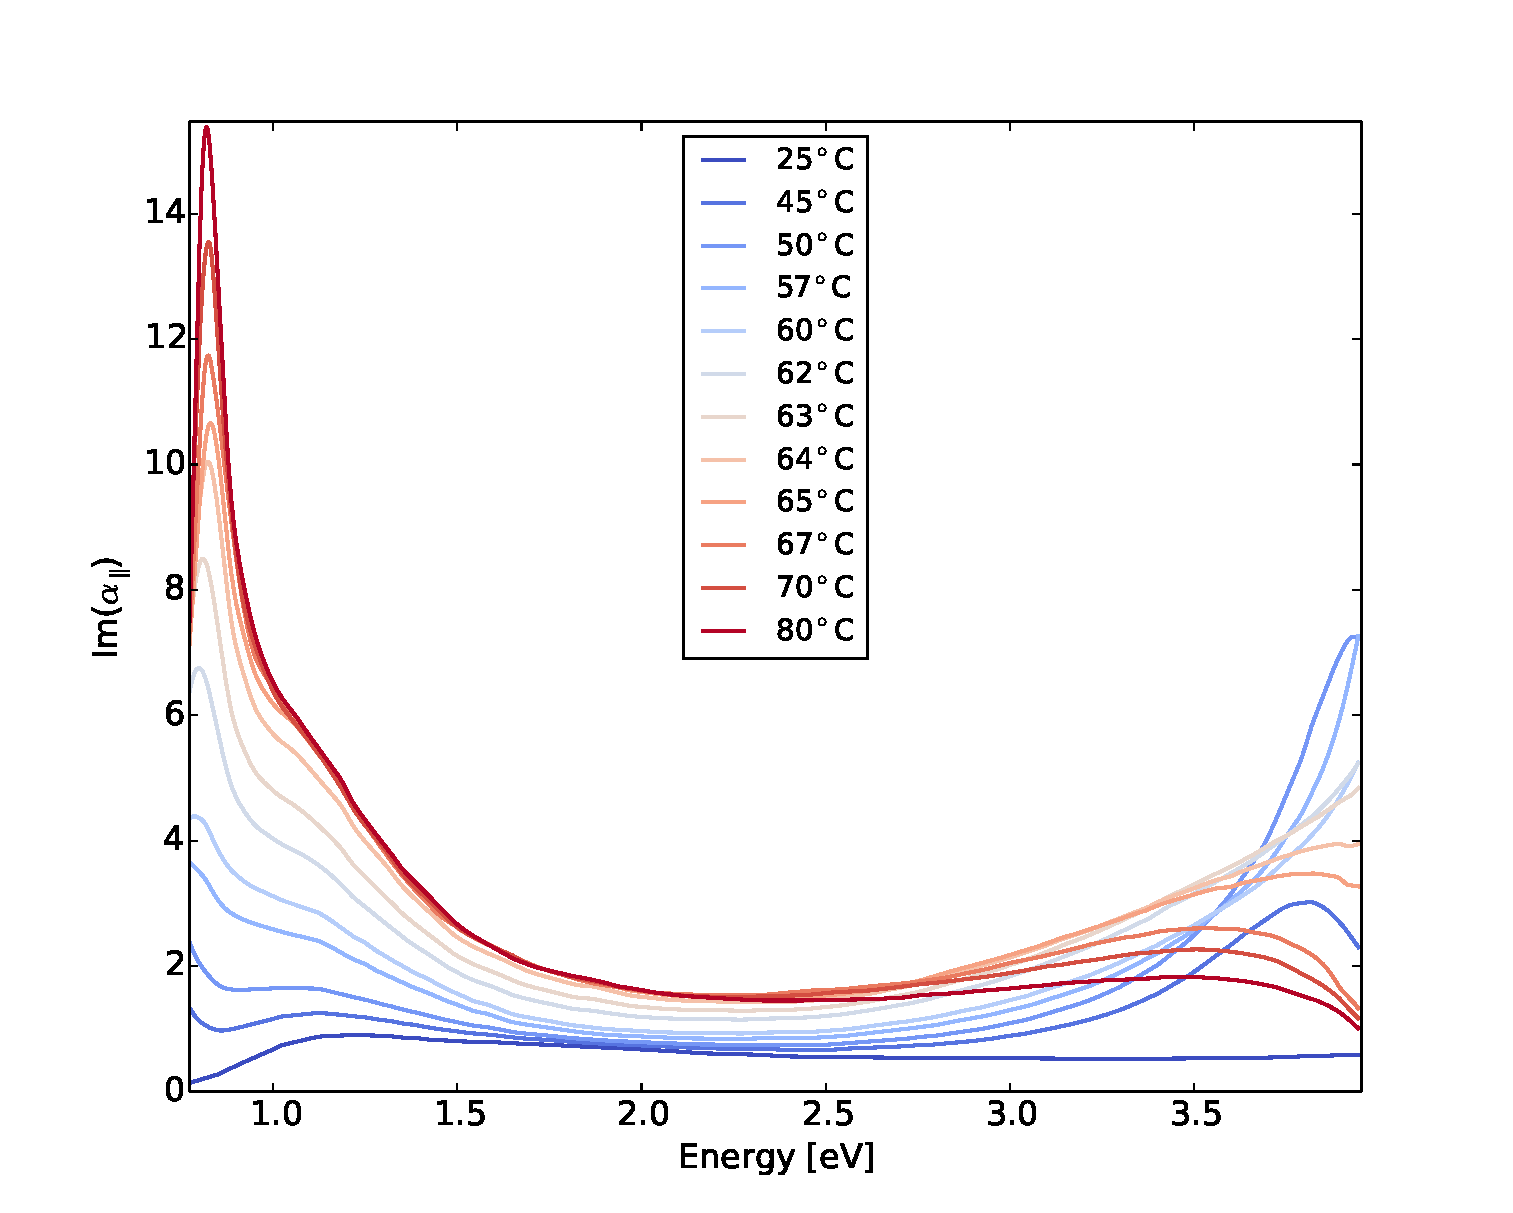
\includegraphics[width=\textwidth]{Results/Sim2/im_alpha_parallel.pdf}
        \caption{}
        \label{fig:2}
    \end{subfigure}
    %\hfill
    \begin{subfigure}[b]{0.49\textwidth}
        \centering
        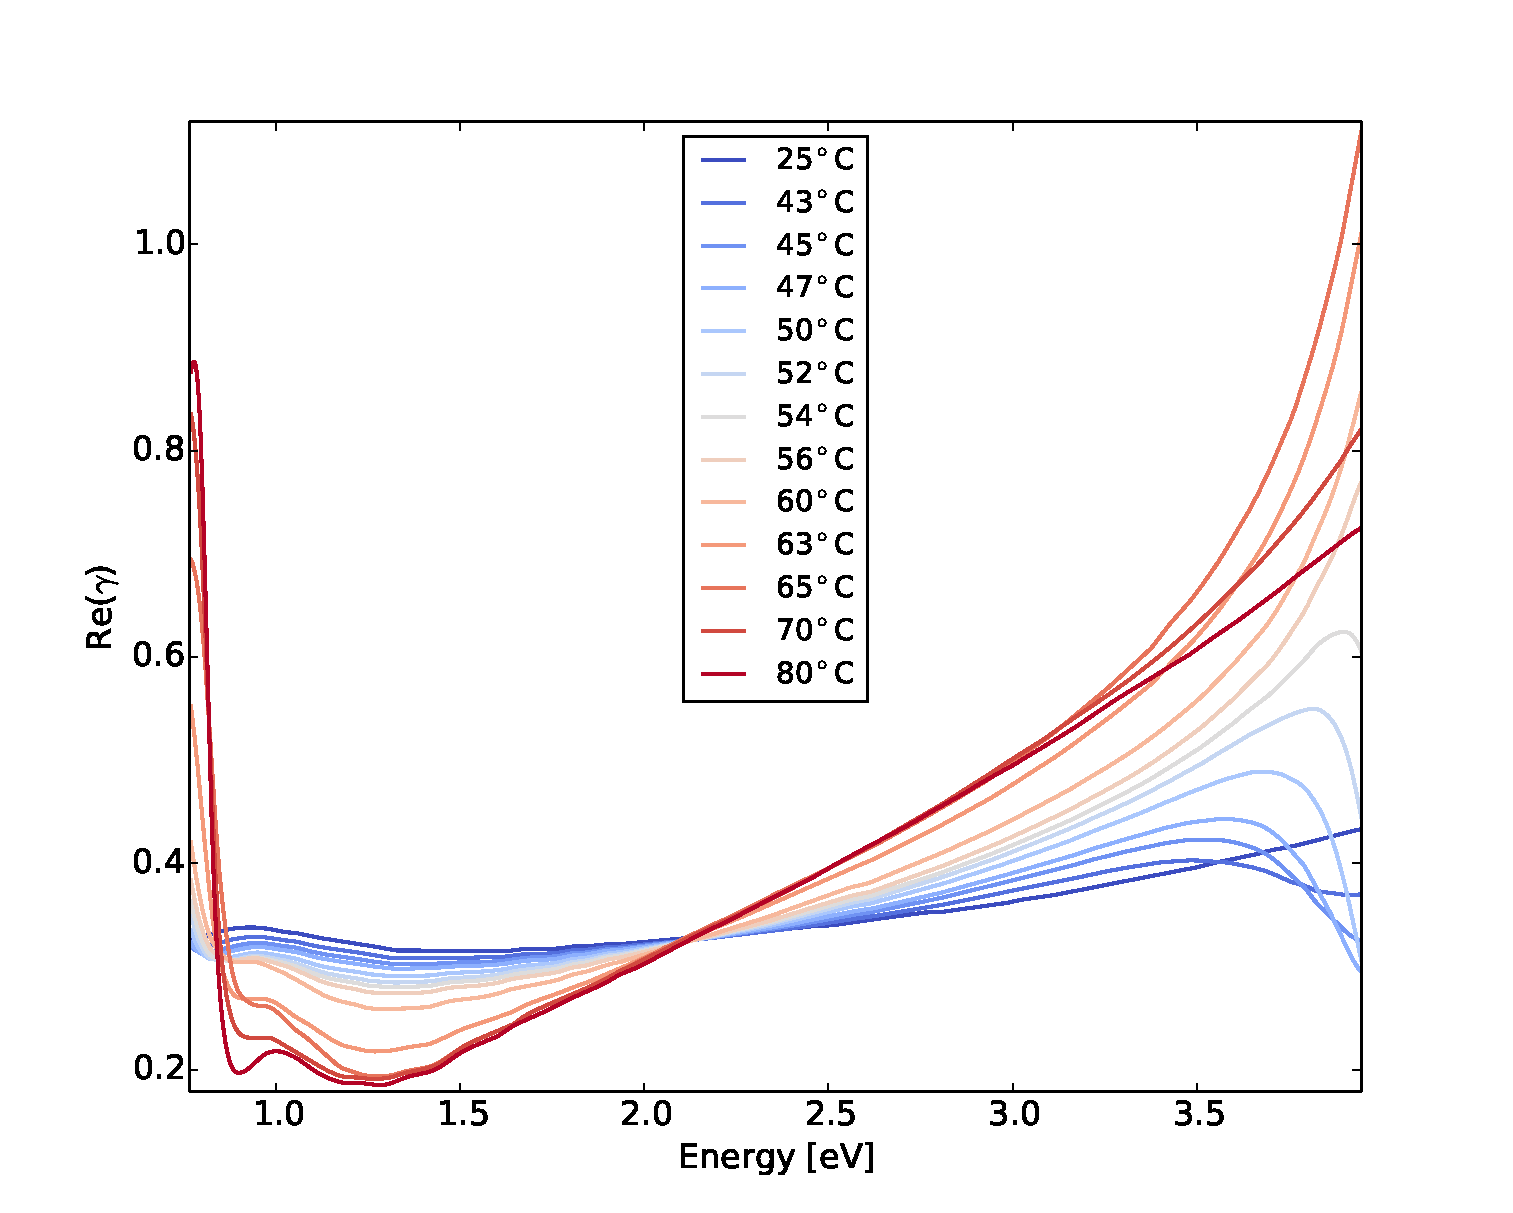
\includegraphics[width=\textwidth]{Results/Sim2/re_gamma.pdf}
        \caption{}
        \label{fig:2}
    \end{subfigure}
    %\hfill
    \begin{subfigure}[b]{0.49\textwidth}
        \centering
        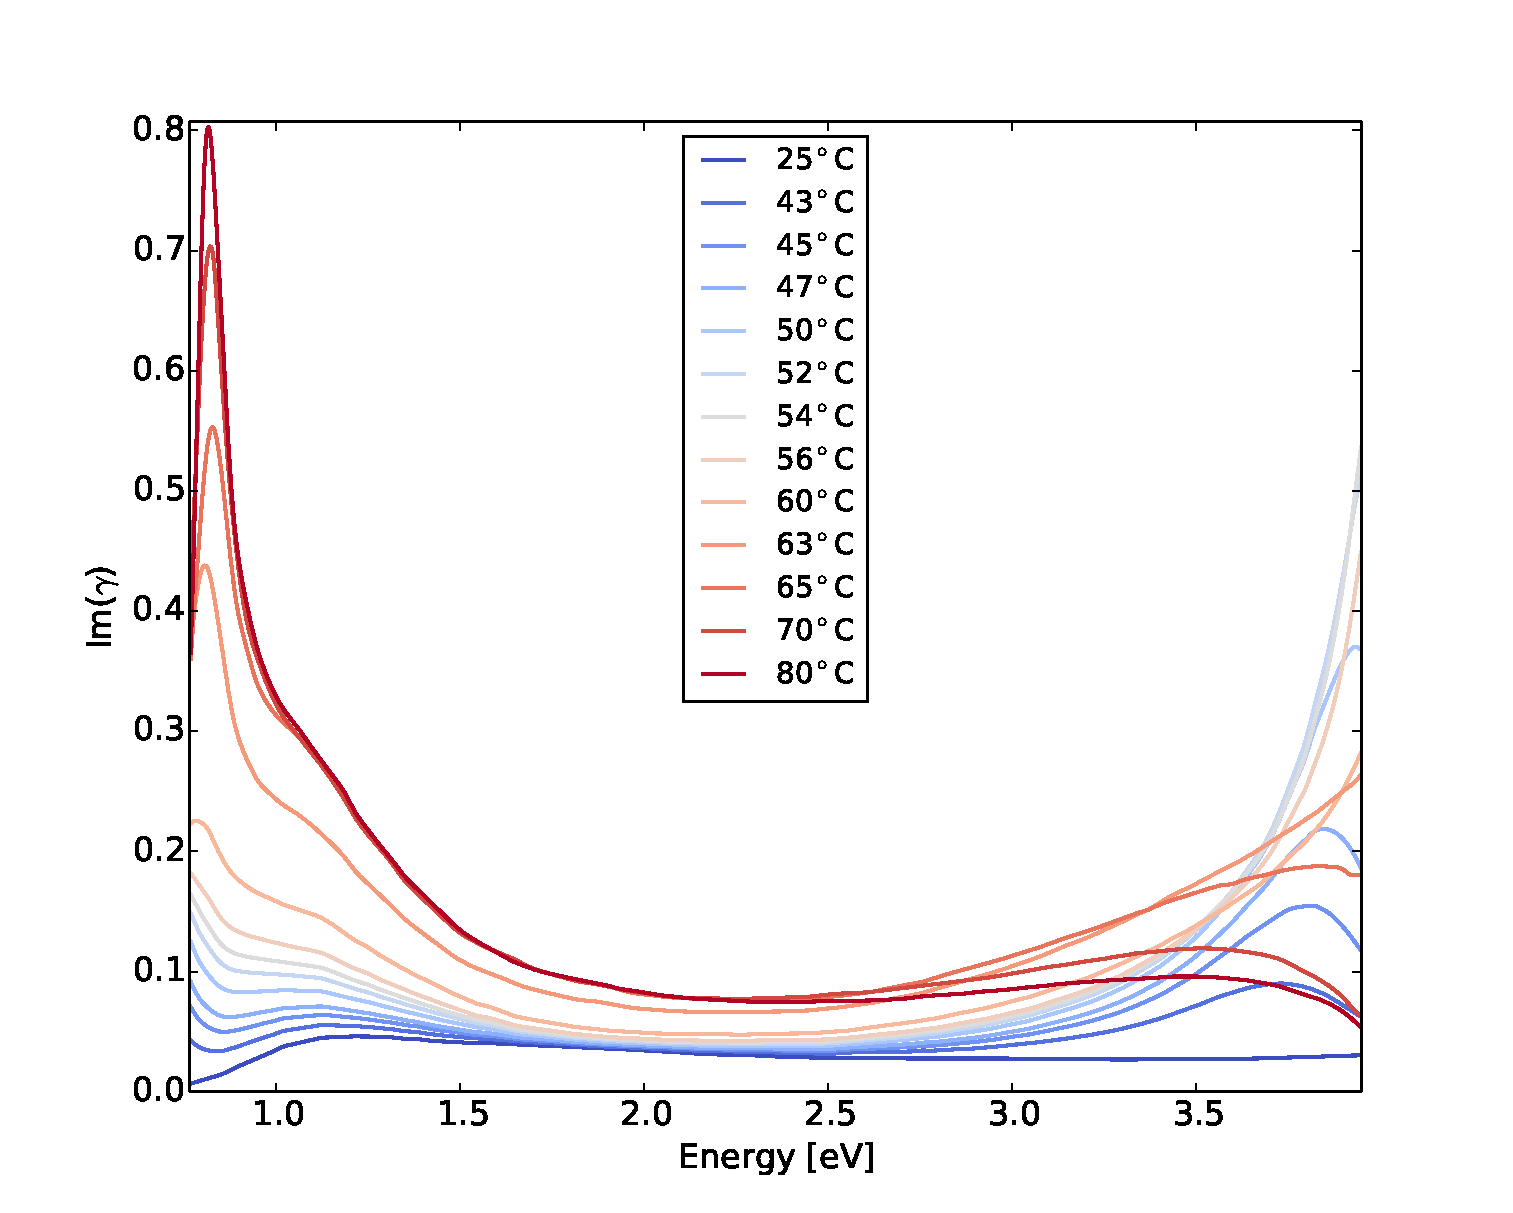
\includegraphics[width=\textwidth]{Results/Sim2/im_gamma.pdf}
        \caption{}
        \label{fig:2}
    \end{subfigure}
    \caption{Relative reflectance $\Delta R/R$}
    \label{fig:}
\end{figure}
%
%
\begin{figure}
    \centering
    \begin{subfigure}[b]{0.49\textwidth}
        \centering
        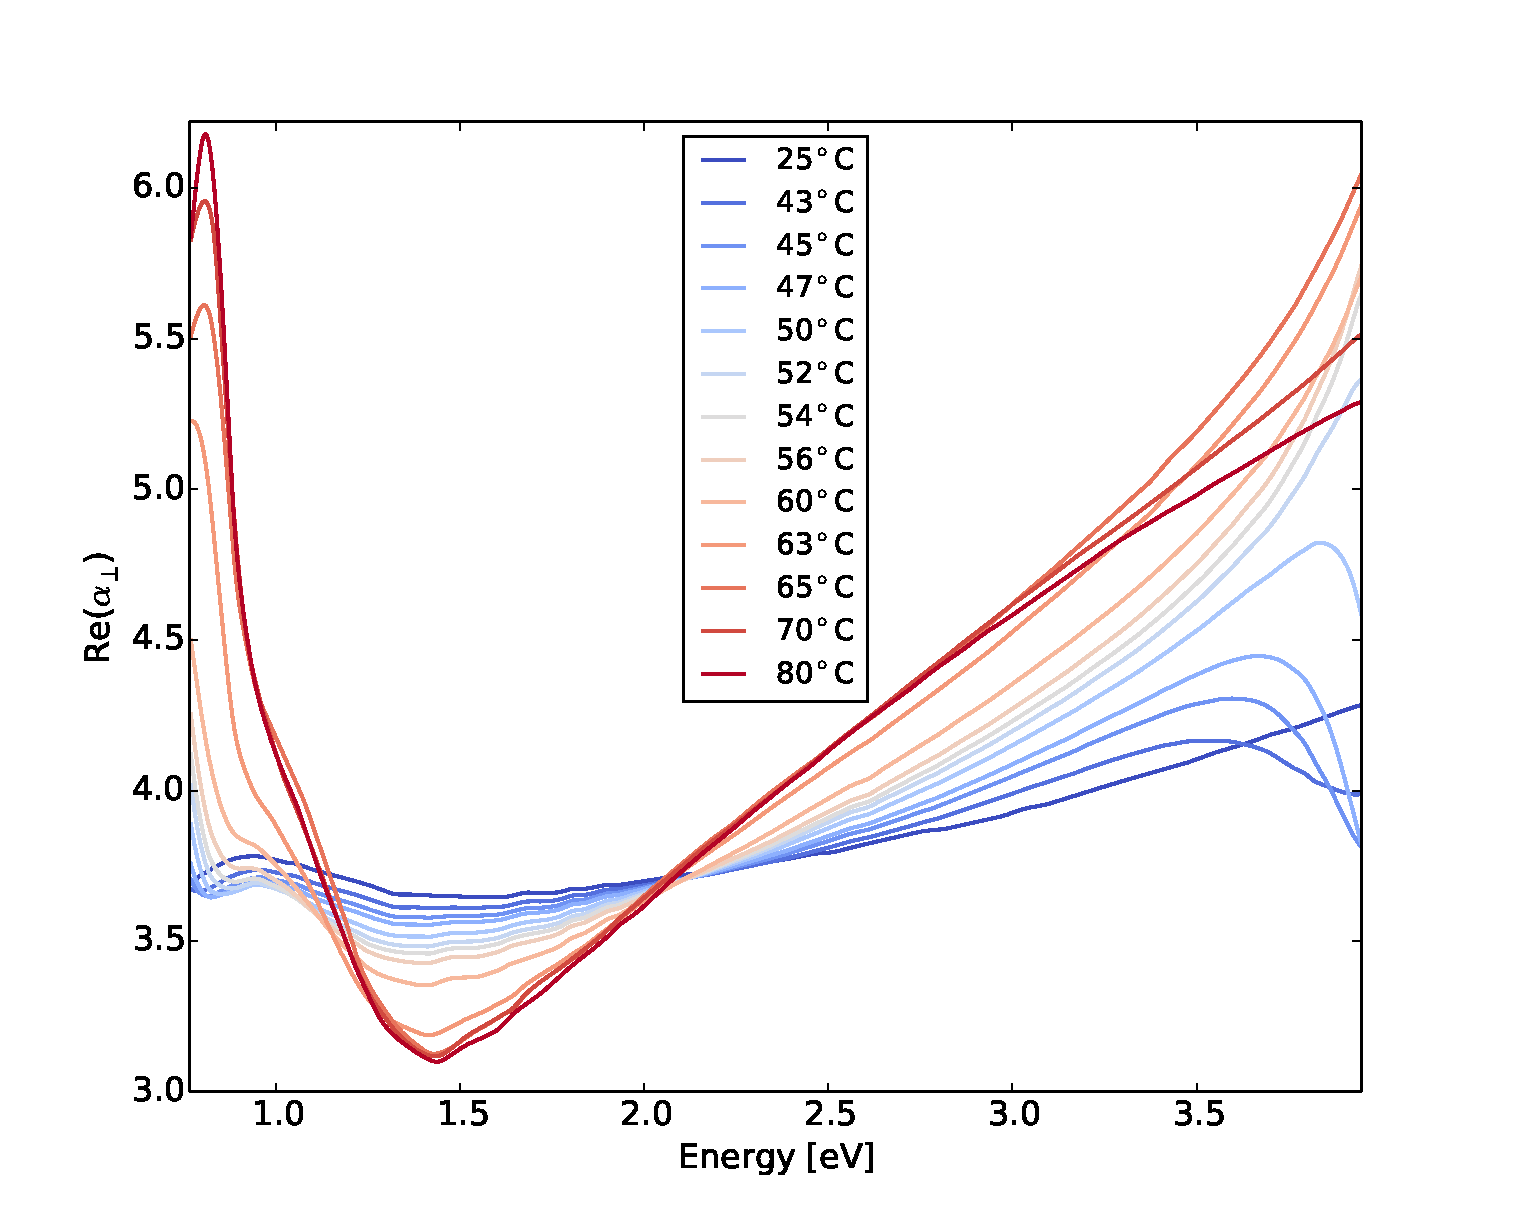
\includegraphics[width=\textwidth]{Results/Sim2/re_alpha_perp.pdf}
        \caption{}
        \label{fig:}
    \end{subfigure}
    %\hfill
    \begin{subfigure}[b]{0.49\textwidth}
        \centering
        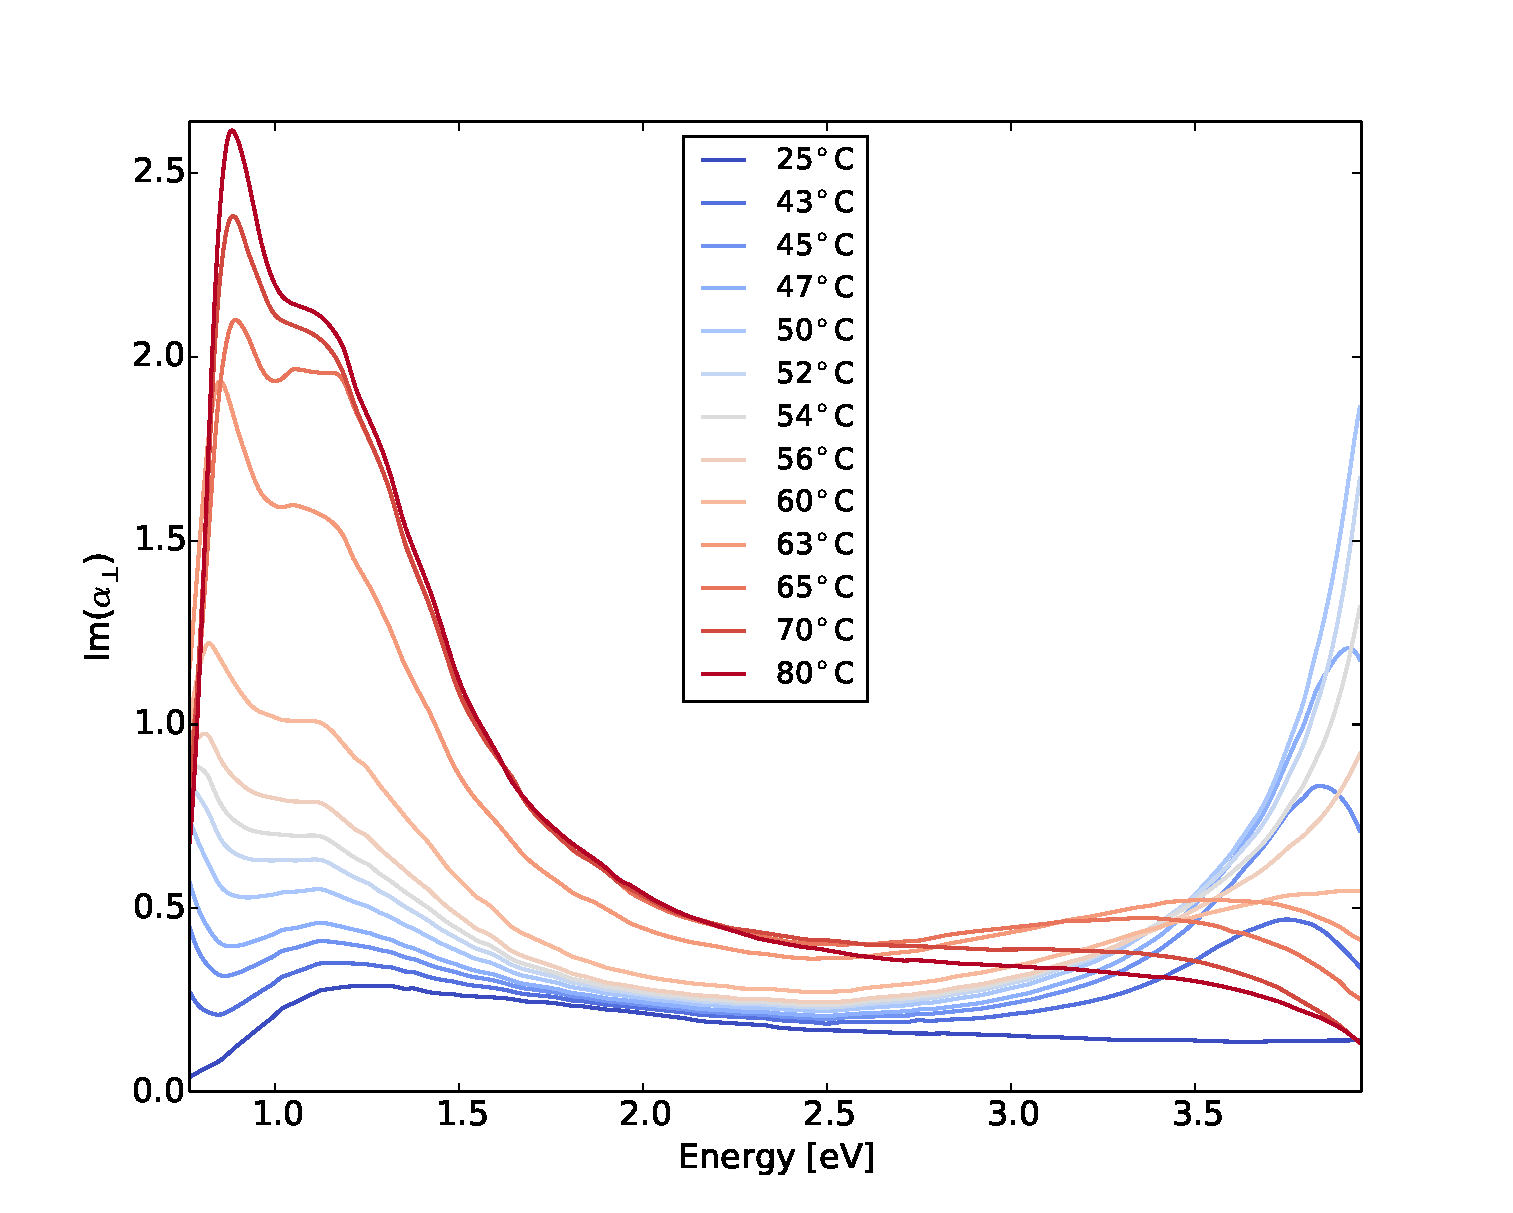
\includegraphics[width=\textwidth]{Results/Sim2/im_alpha_perp.pdf}
        \caption{}
        \label{fig:}
    \end{subfigure}
    %\hfill
    \begin{subfigure}[b]{0.49\textwidth}
        \centering
        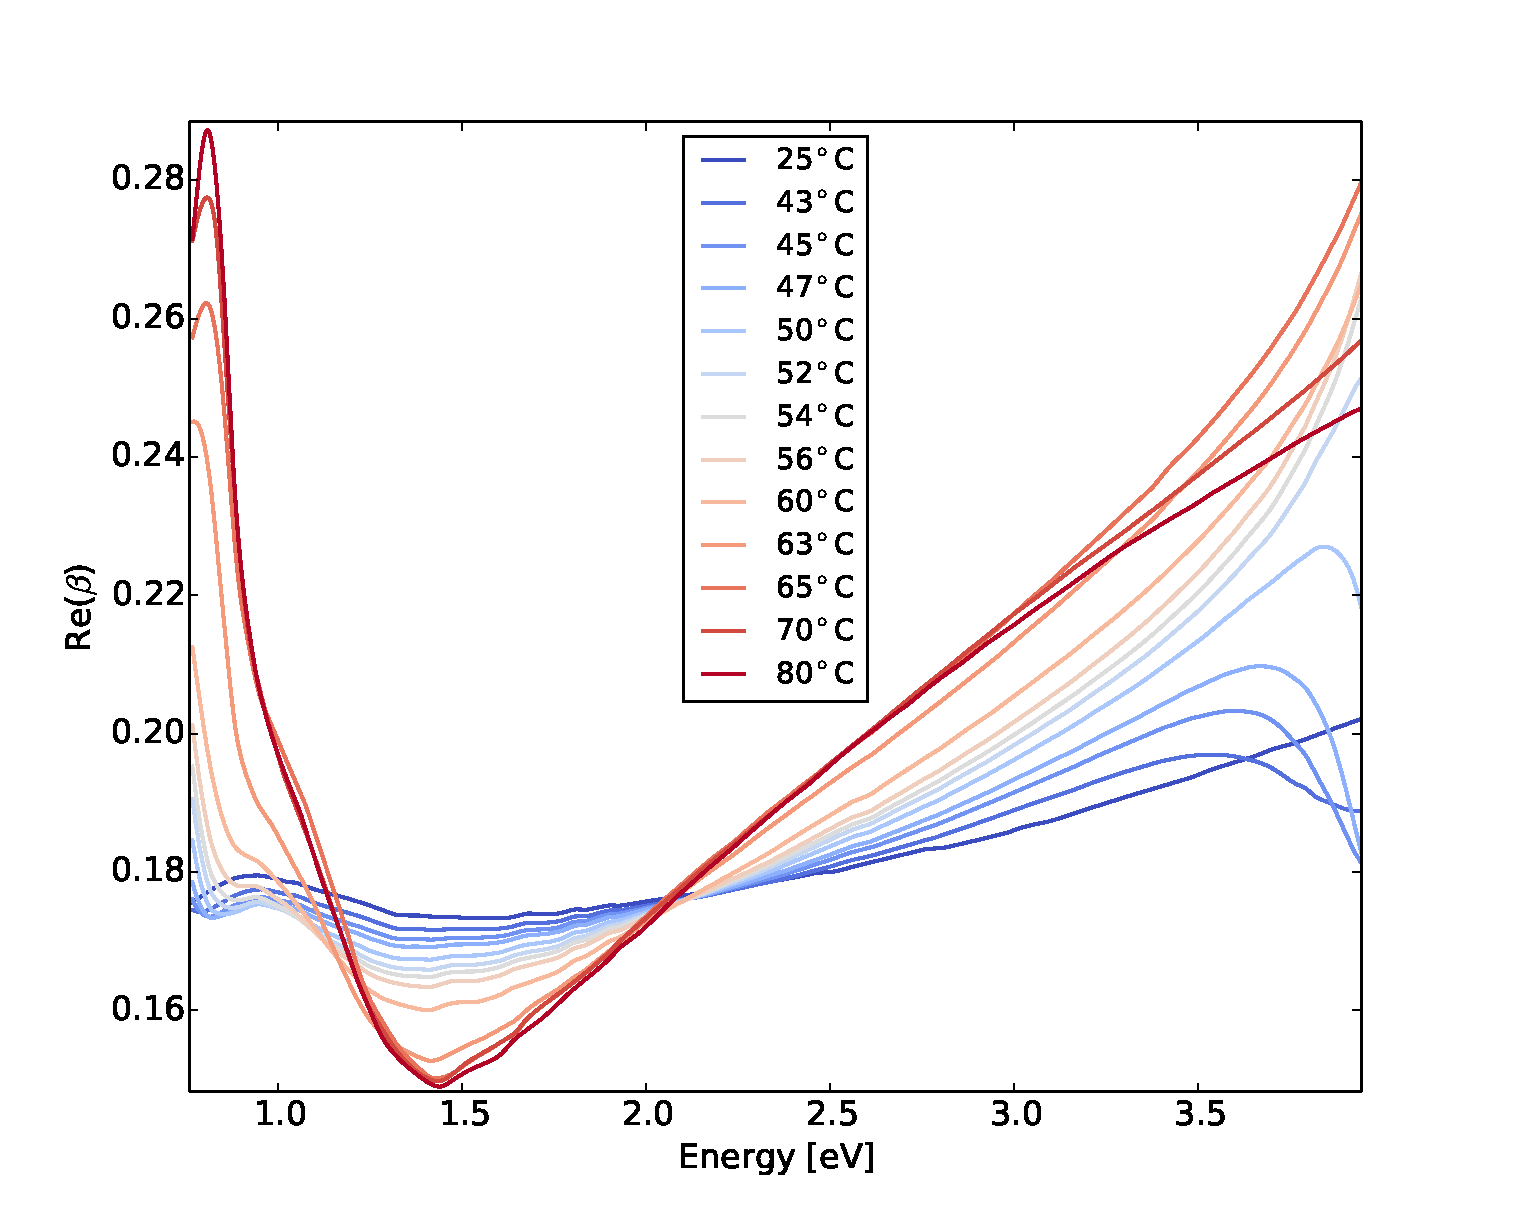
\includegraphics[width=\textwidth]{Results/Sim2/re_beta.pdf}
        \caption{}
        \label{fig:2}
    \end{subfigure}
    %\hfill
    \begin{subfigure}[b]{0.49\textwidth}
        \centering
        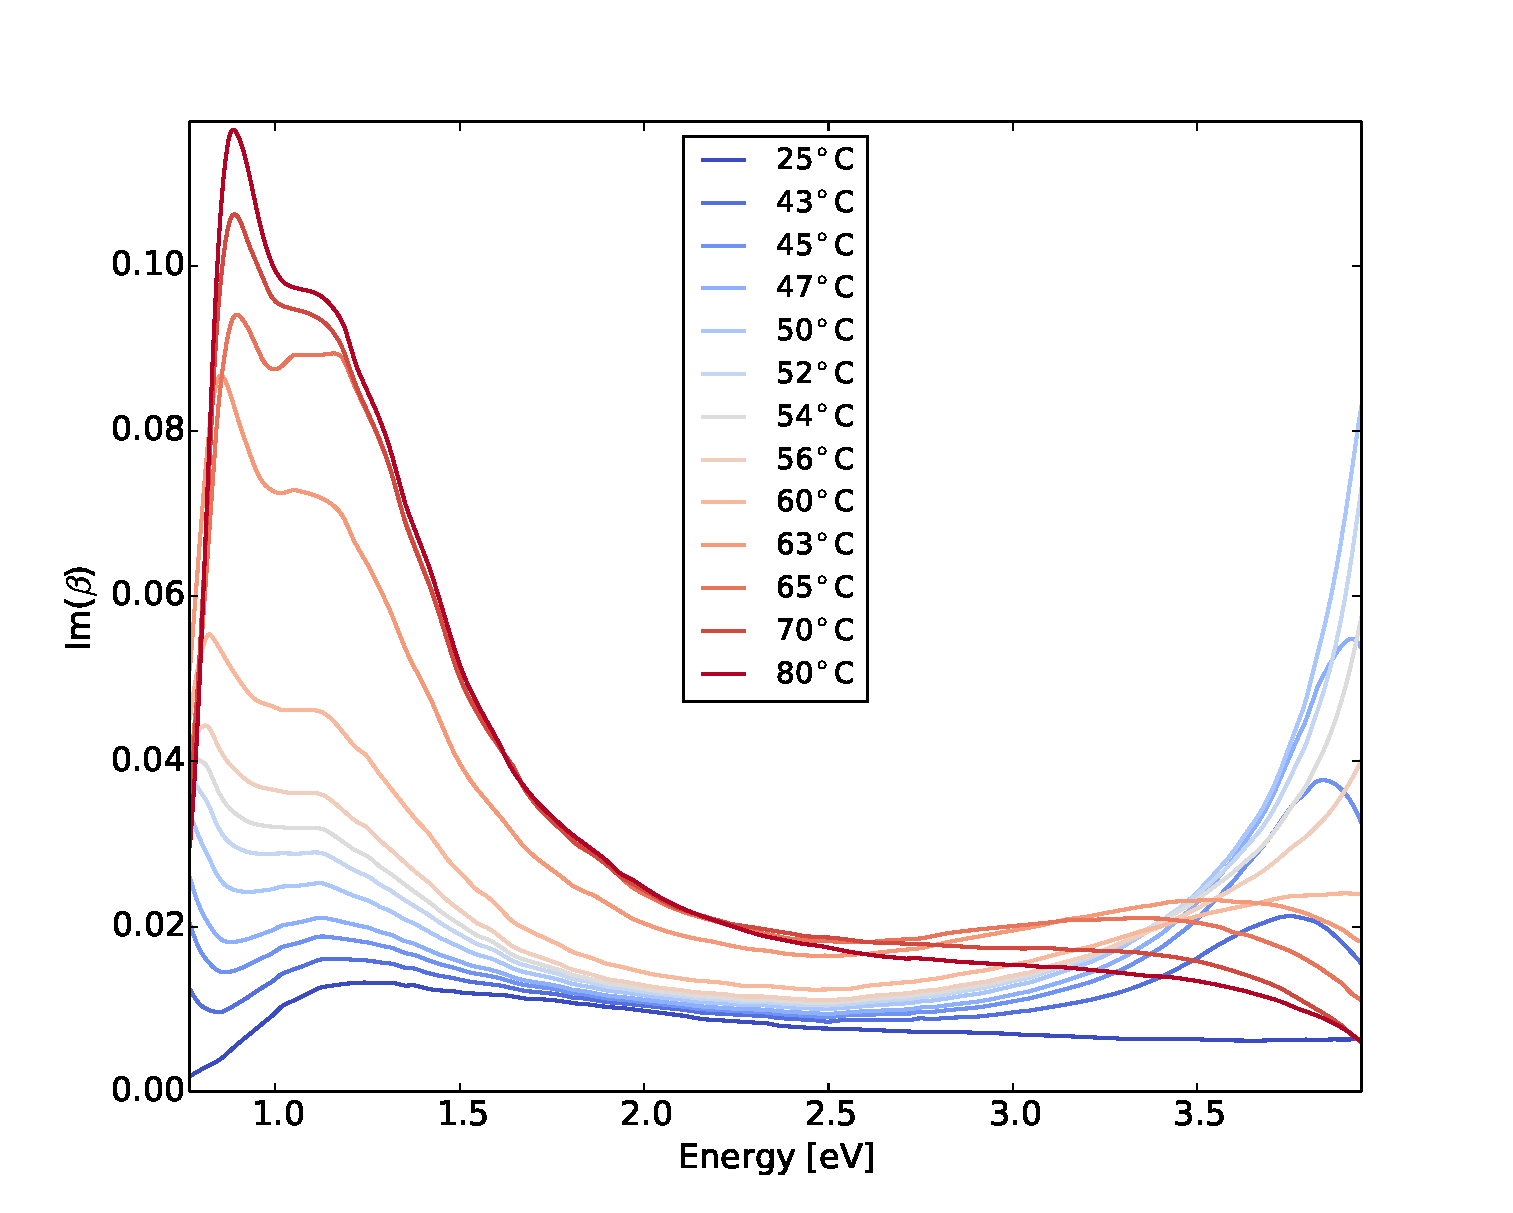
\includegraphics[width=\textwidth]{Results/Sim2/im_beta.pdf}
        \caption{}
        \label{fig:2}
    \end{subfigure}
    \caption{Relative reflectance $\Delta R/R$}
    \label{fig:}
\end{figure}
%



\subsection{Simulation 3; $R = 15$nm, p-polarized incident light}
%
\begin{figure}
    \centering
    \begin{subfigure}[b]{0.49\textwidth}
        \centering
        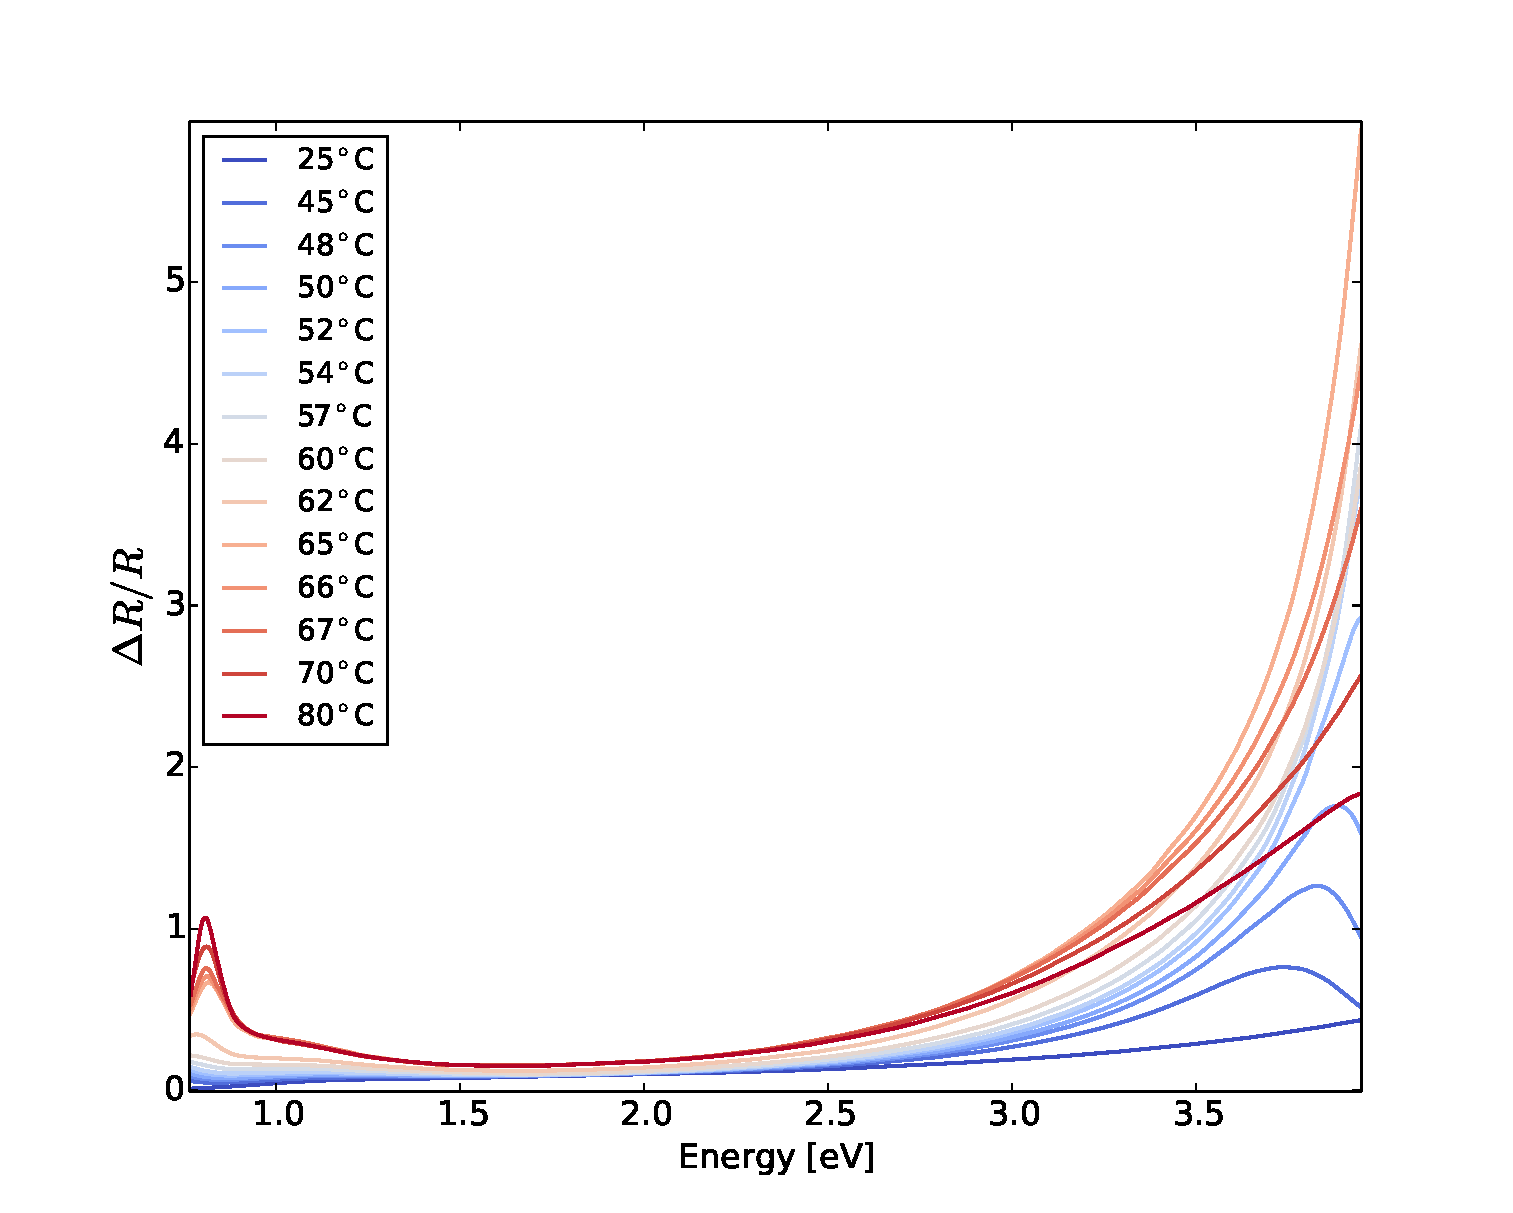
\includegraphics[width=\textwidth]{Results/Sim3/dR.pdf}
        \caption{}
        \label{fig:}
    \end{subfigure}
    %\hfill
    \begin{subfigure}[b]{0.49\textwidth}
        \centering
        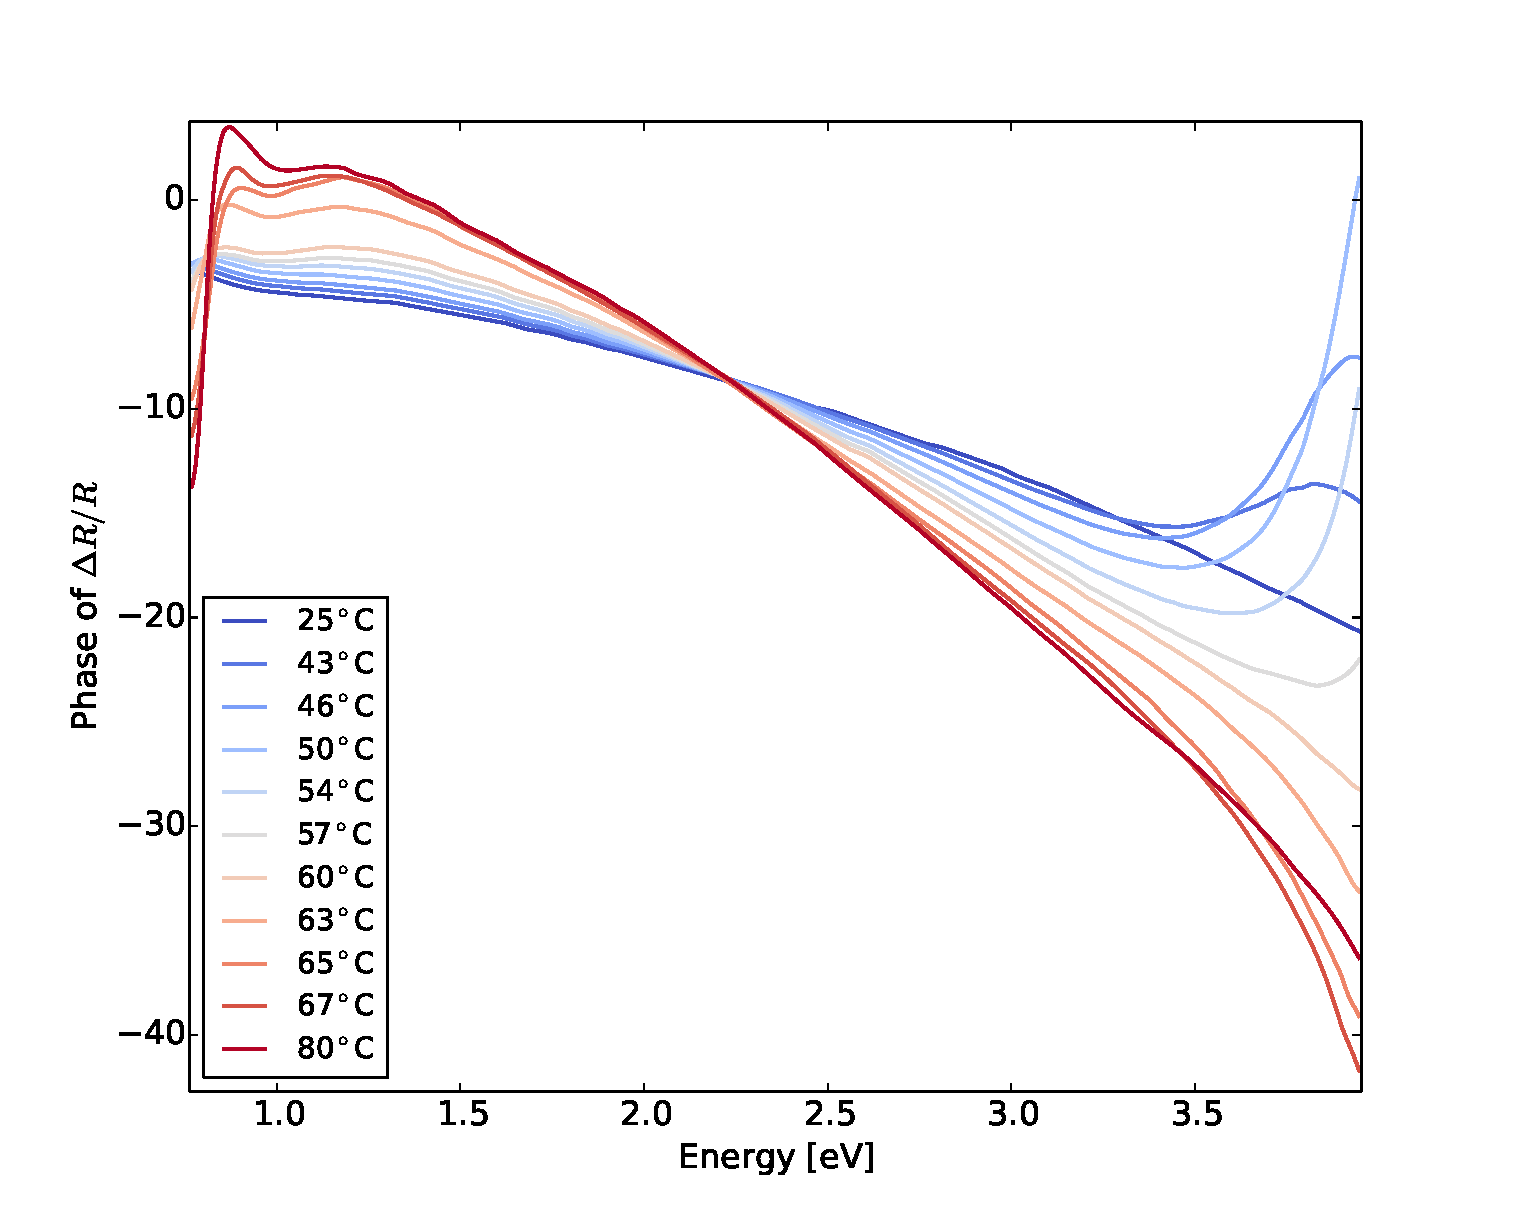
\includegraphics[width=\textwidth]{Results/Sim3/dRphase.pdf}
        \caption{}
        \label{fig:}
    \end{subfigure}
    \caption{Relative reflectance $\Delta R/R$}
    \label{fig:1}
\end{figure}
%
%
\begin{figure}
    \centering
    \begin{subfigure}[b]{0.49\textwidth}
        \centering
        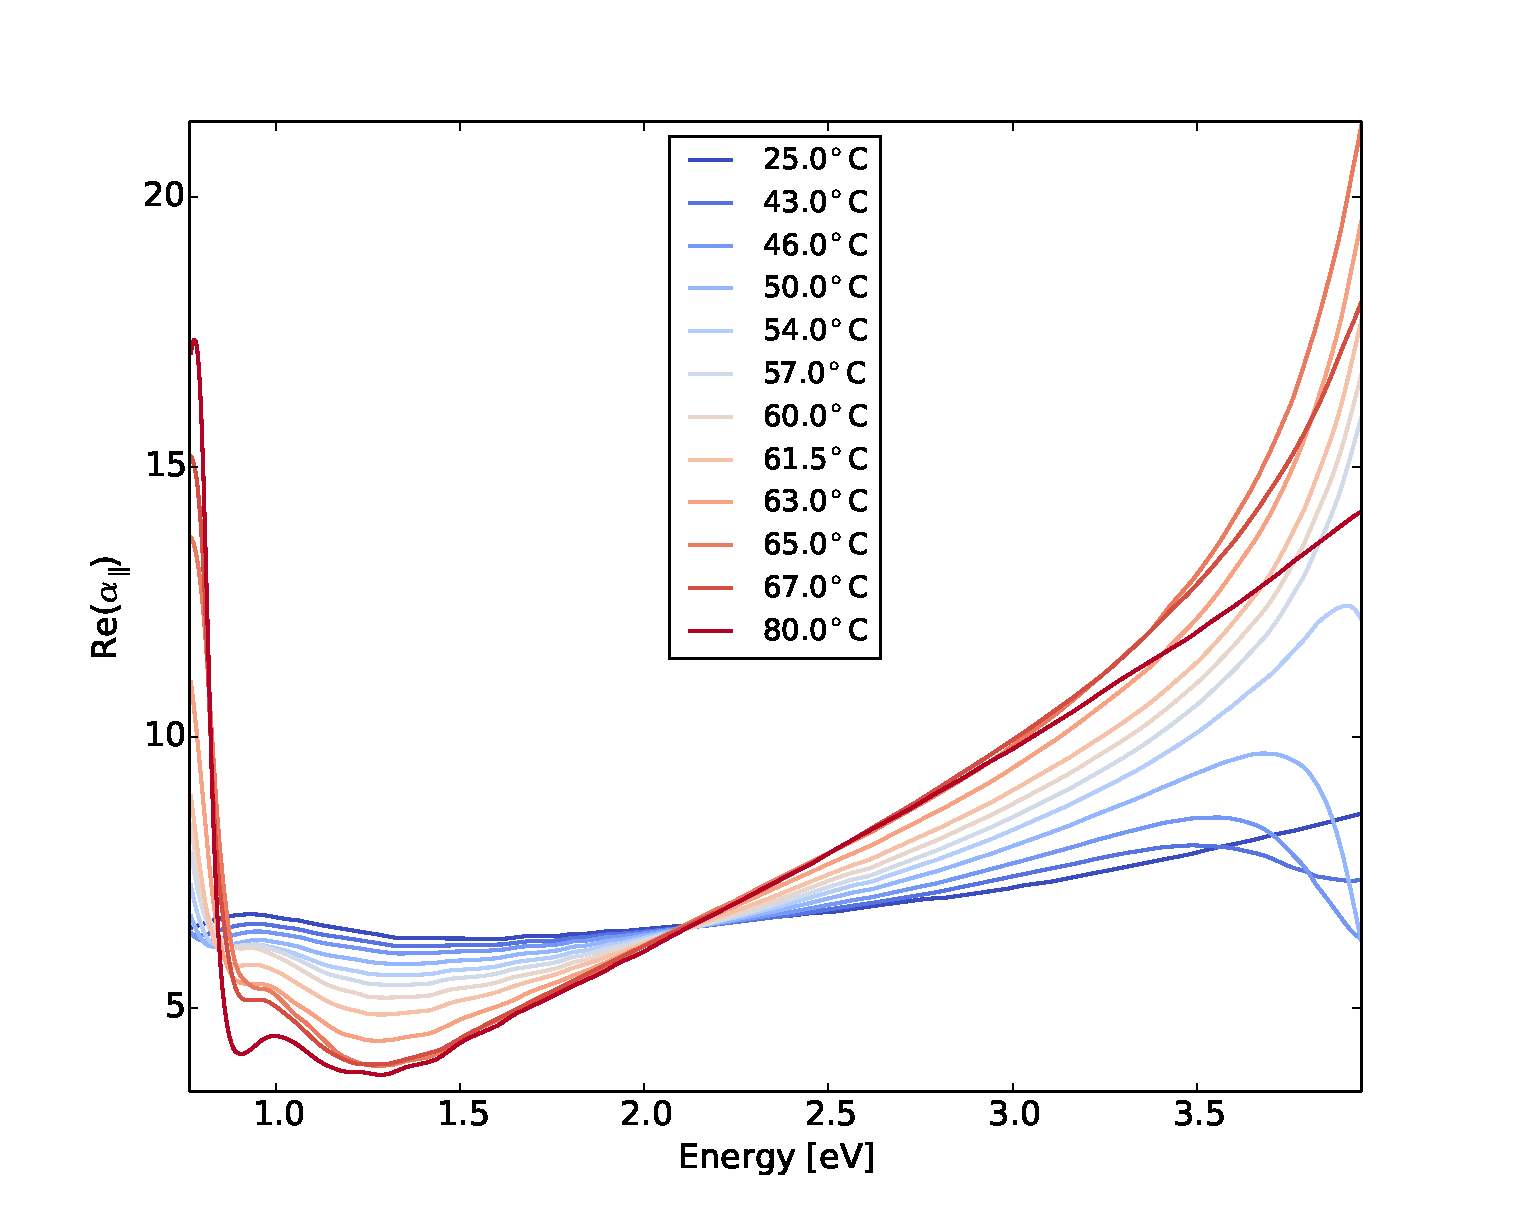
\includegraphics[width=\textwidth]{Results/Sim3/re_alpha_parallel.pdf}
        \caption{}
        \label{fig:2}
    \end{subfigure}
    %\hfill
    \begin{subfigure}[b]{0.49\textwidth}
        \centering
        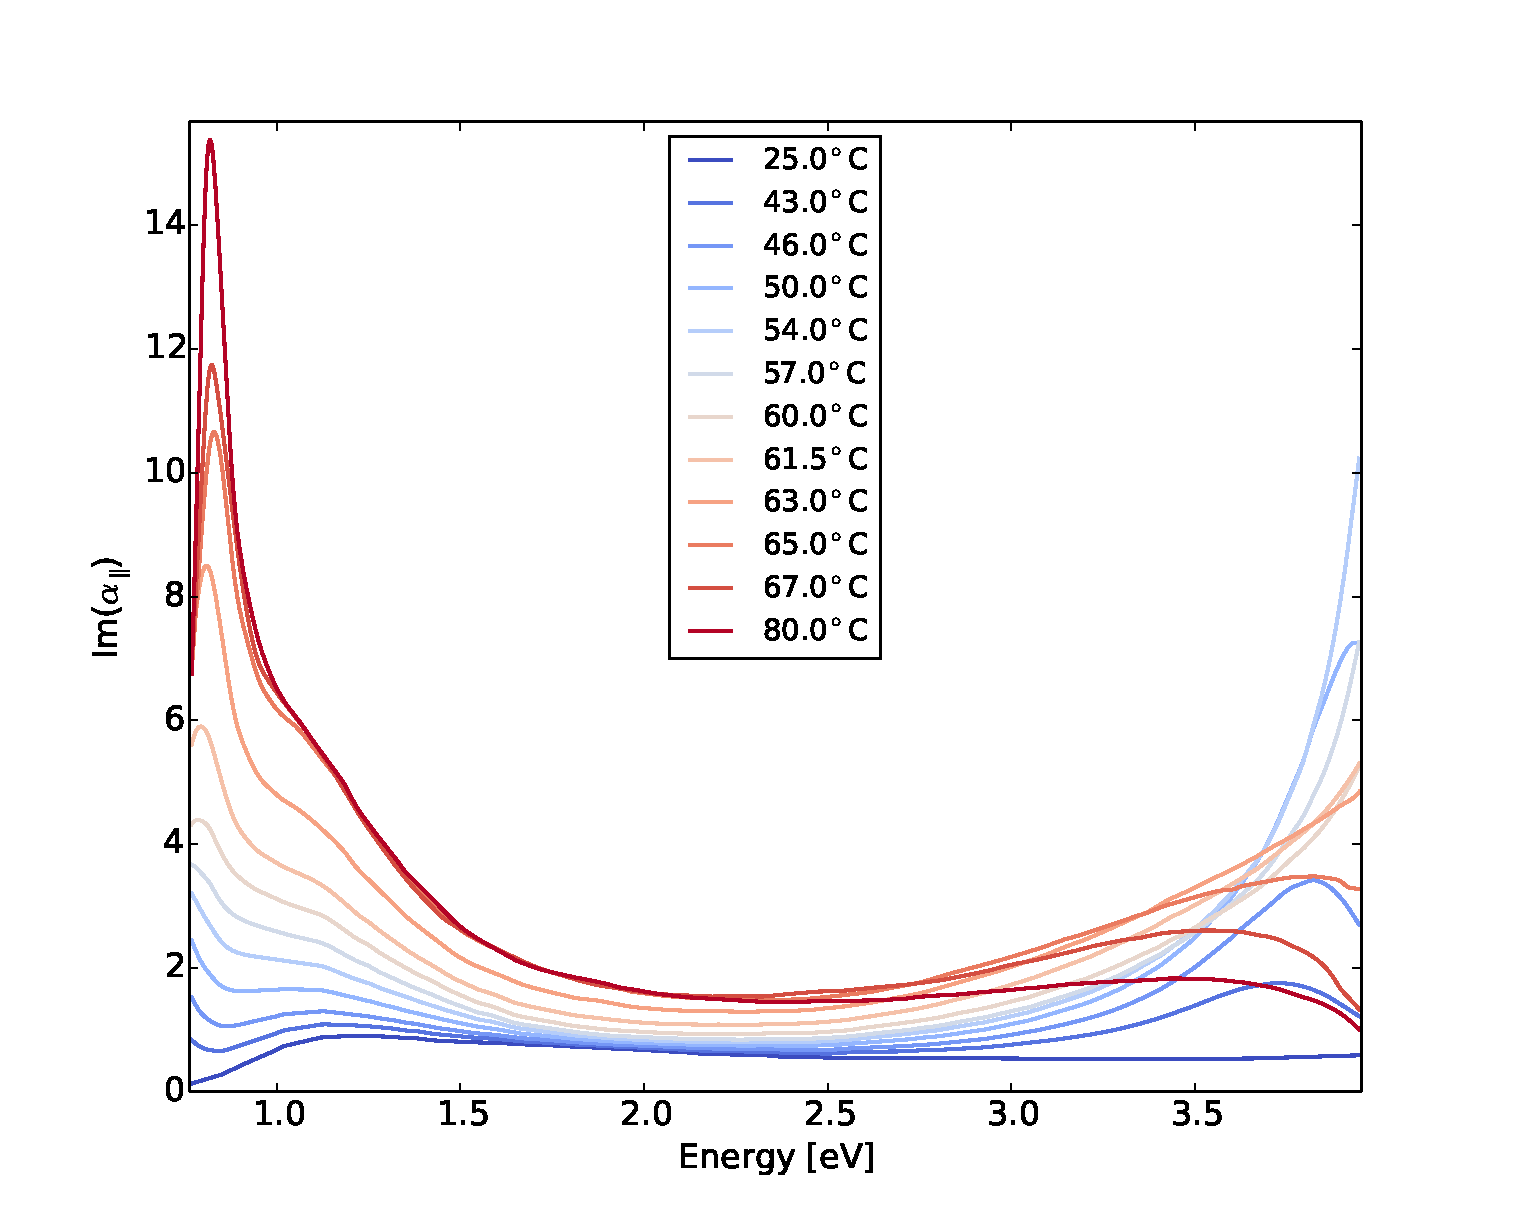
\includegraphics[width=\textwidth]{Results/Sim3/im_alpha_parallel.pdf}
        \caption{}
        \label{fig:2}
    \end{subfigure}
    %\hfill
    \begin{subfigure}[b]{0.49\textwidth}
        \centering
        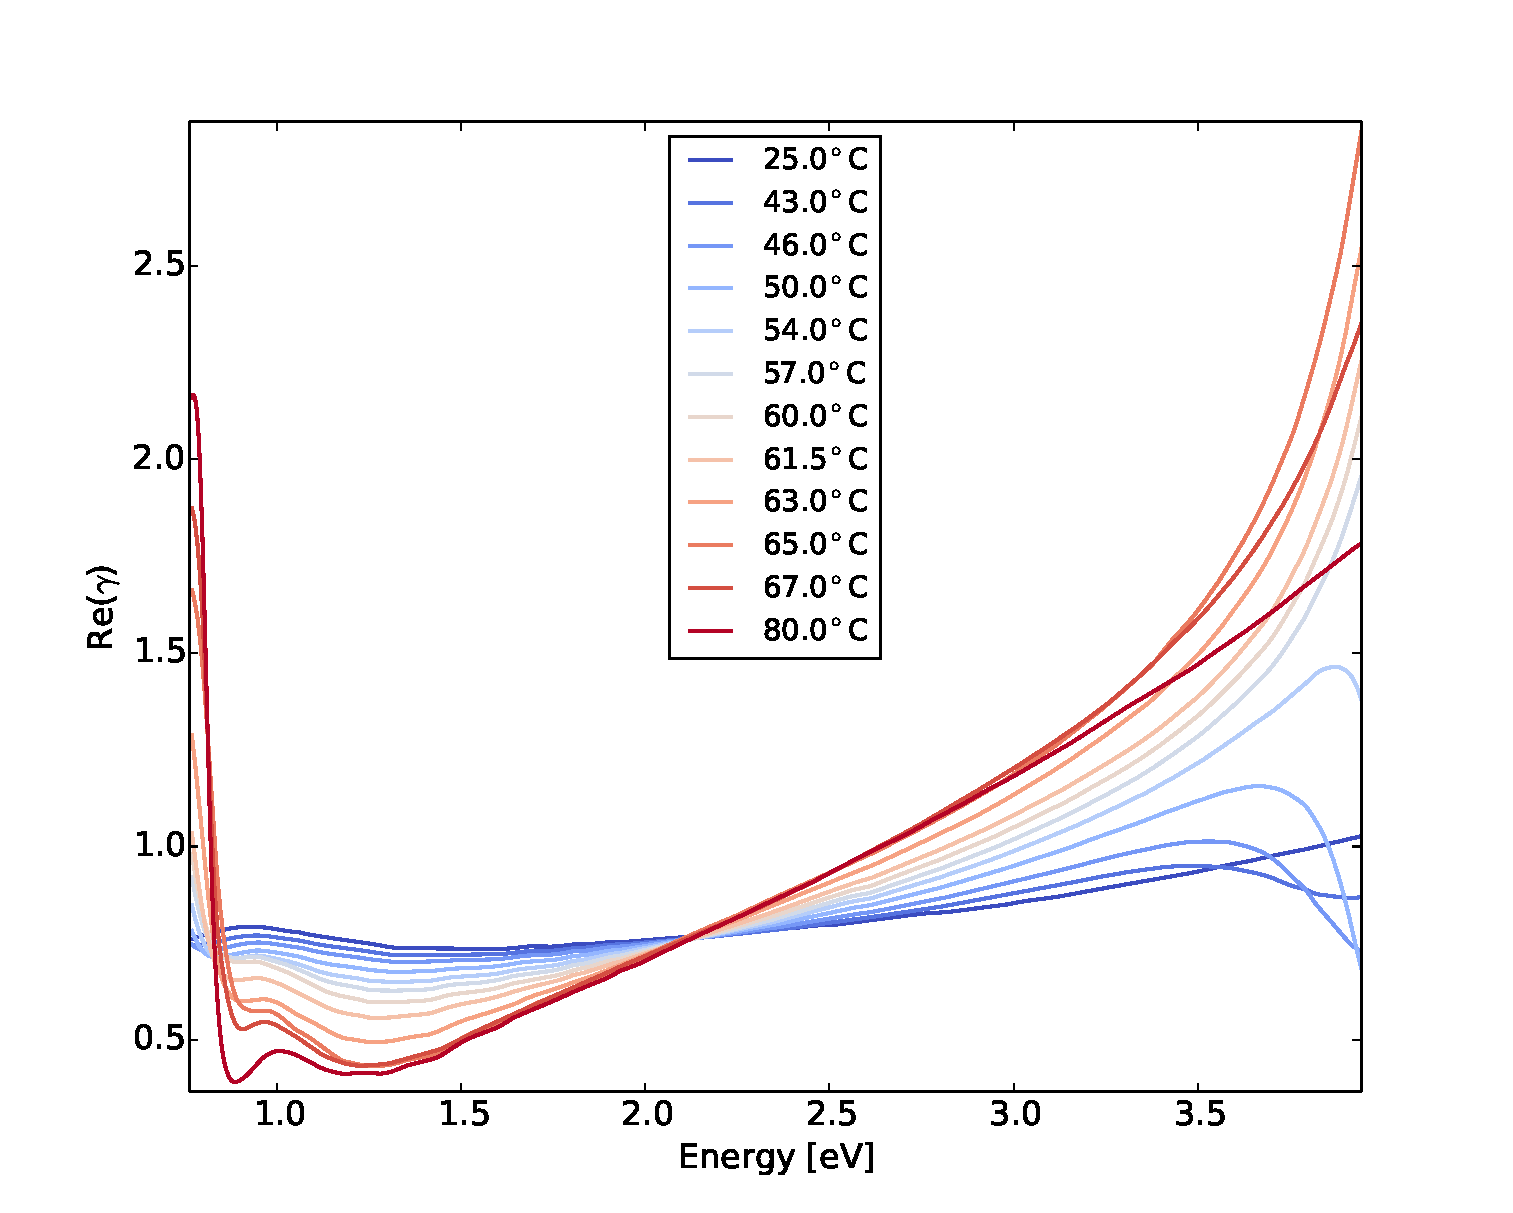
\includegraphics[width=\textwidth]{Results/Sim3/re_gamma.pdf}
        \caption{}
        \label{fig:2}
    \end{subfigure}
    %\hfill
    \begin{subfigure}[b]{0.49\textwidth}
        \centering
        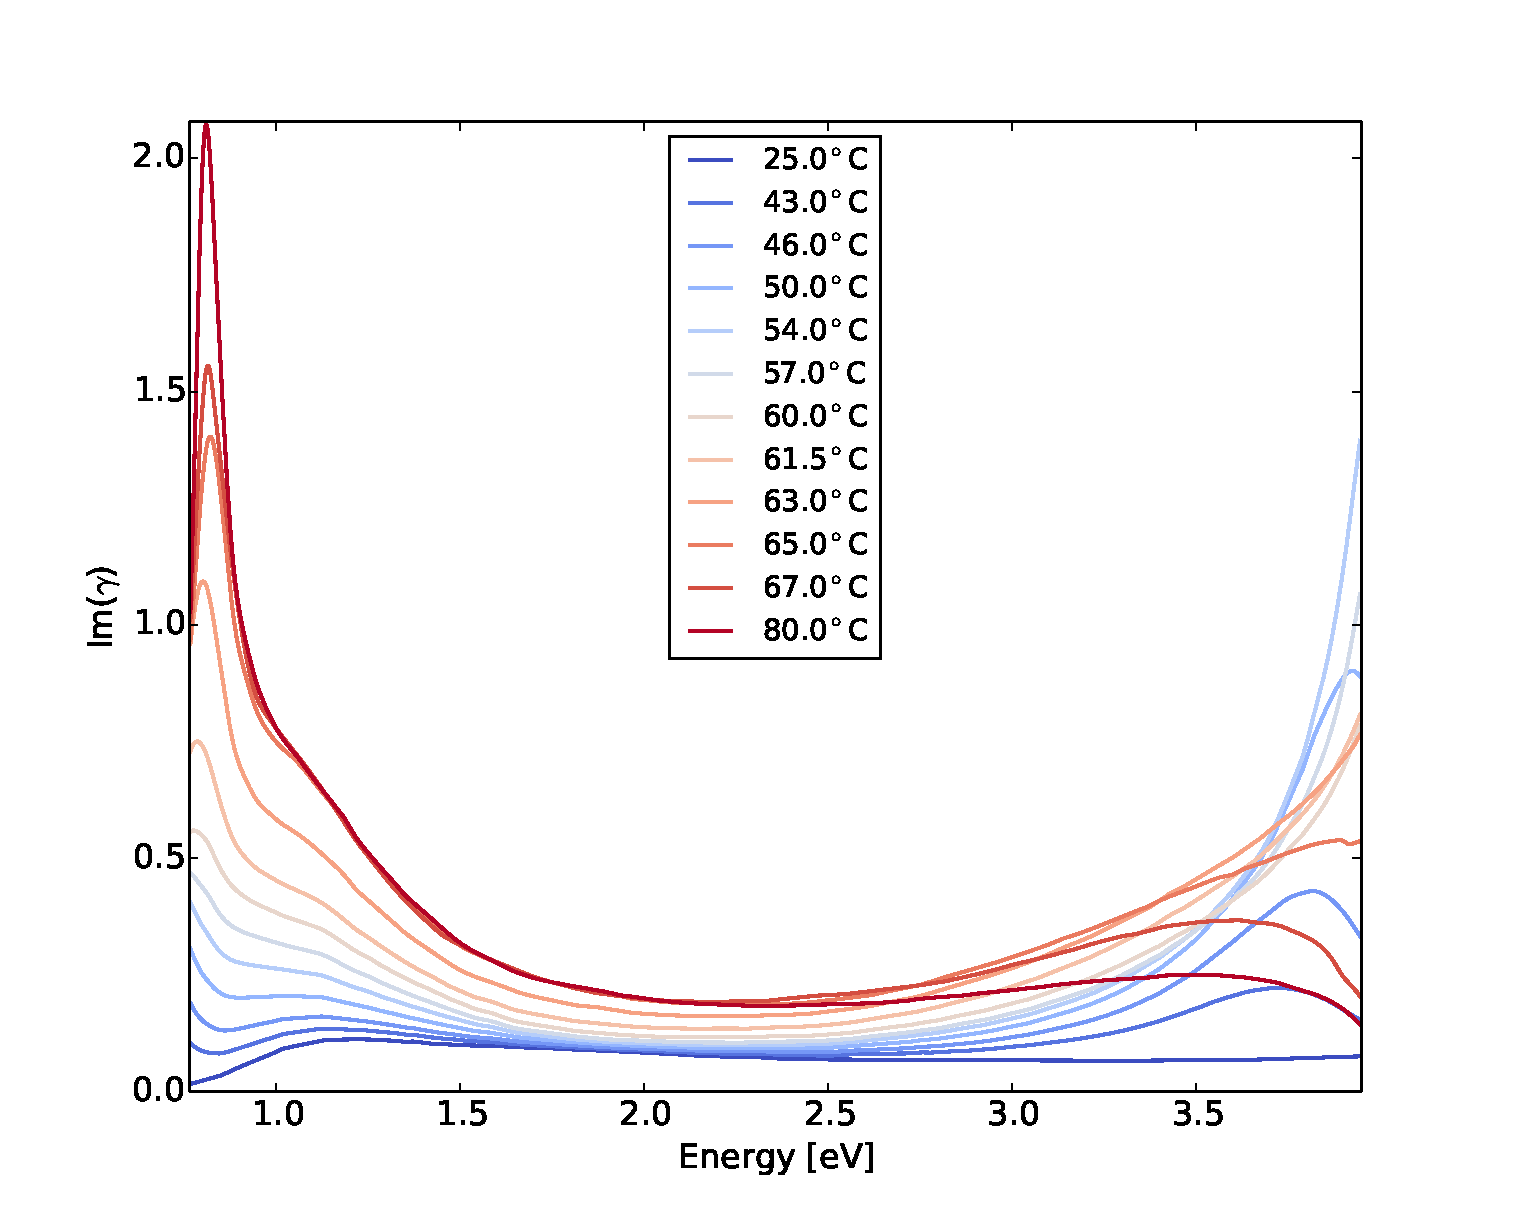
\includegraphics[width=\textwidth]{Results/Sim3/im_gamma.pdf}
        \caption{}
        \label{fig:2}
    \end{subfigure}
    \caption{Relative reflectance $\Delta R/R$}
    \label{fig:}
\end{figure}
%
%
\begin{figure}
    \centering
    \begin{subfigure}[b]{0.49\textwidth}
        \centering
        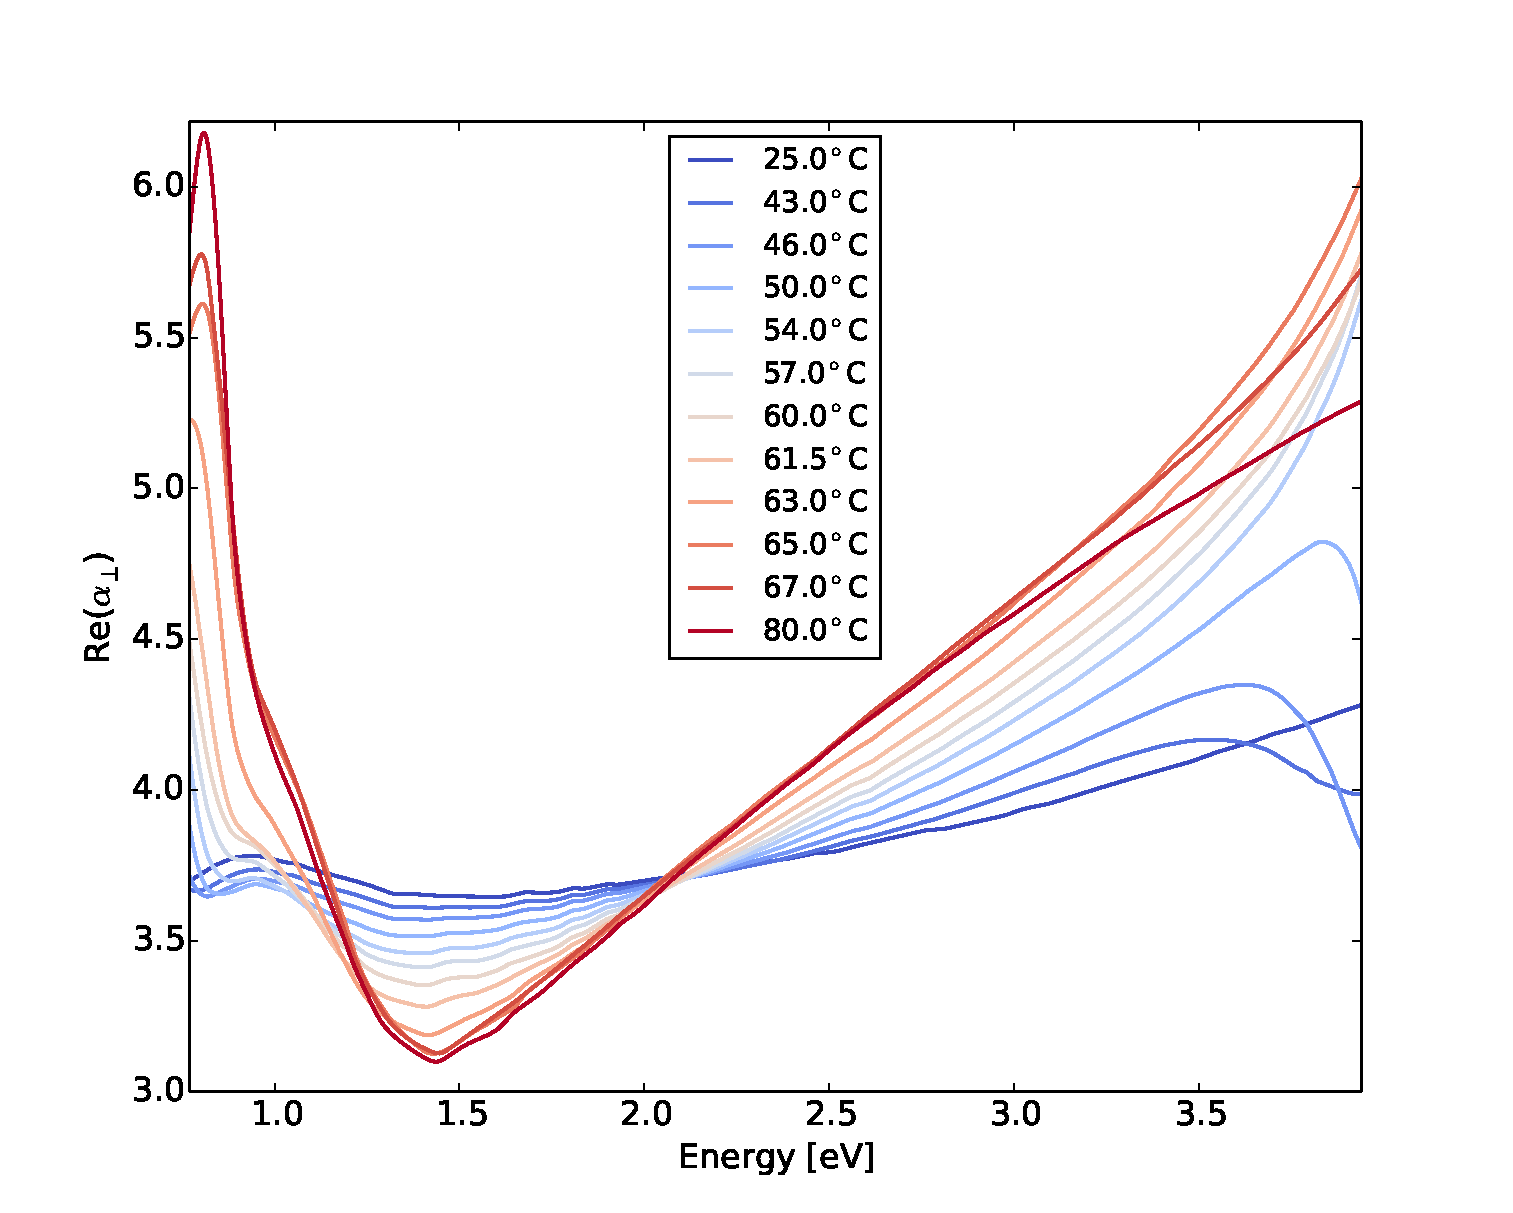
\includegraphics[width=\textwidth]{Results/Sim3/re_alpha_perp.pdf}
        \caption{}
        \label{fig:}
    \end{subfigure}
    %\hfill
    \begin{subfigure}[b]{0.49\textwidth}
        \centering
        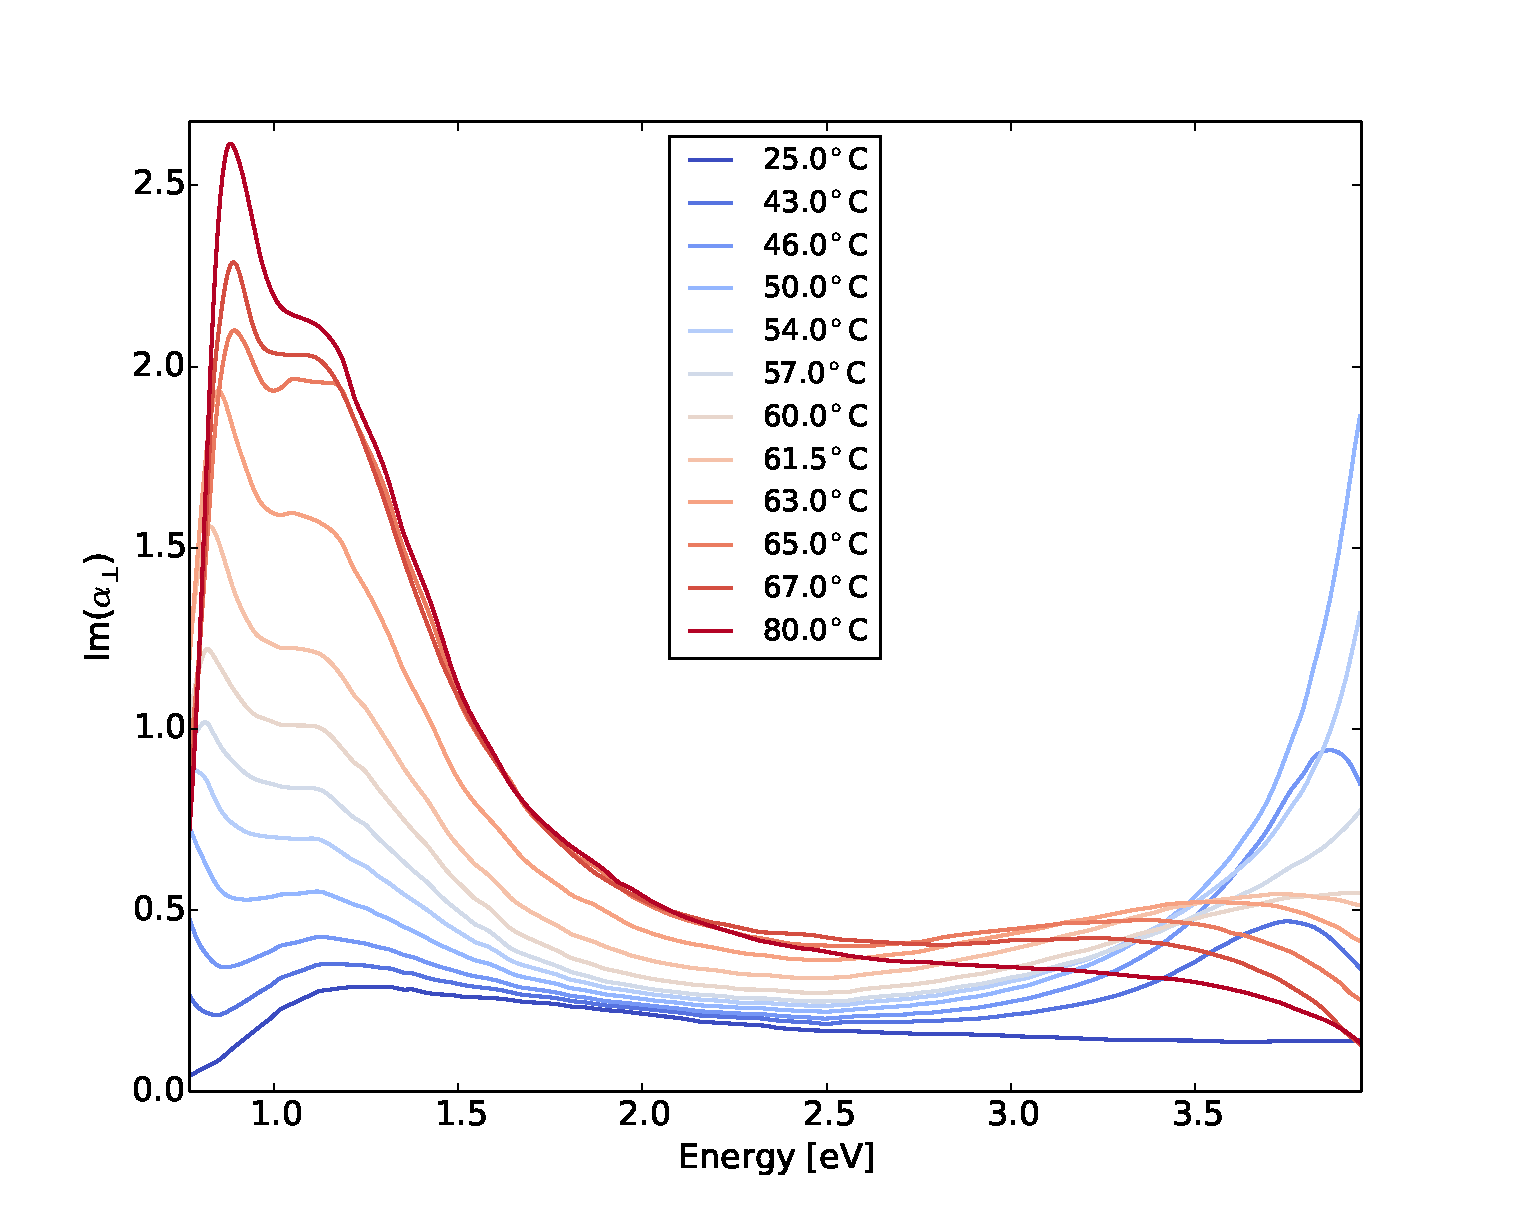
\includegraphics[width=\textwidth]{Results/Sim3/im_alpha_perp.pdf}
        \caption{}
        \label{fig:}
    \end{subfigure}
    %\hfill
    \begin{subfigure}[b]{0.49\textwidth}
        \centering
        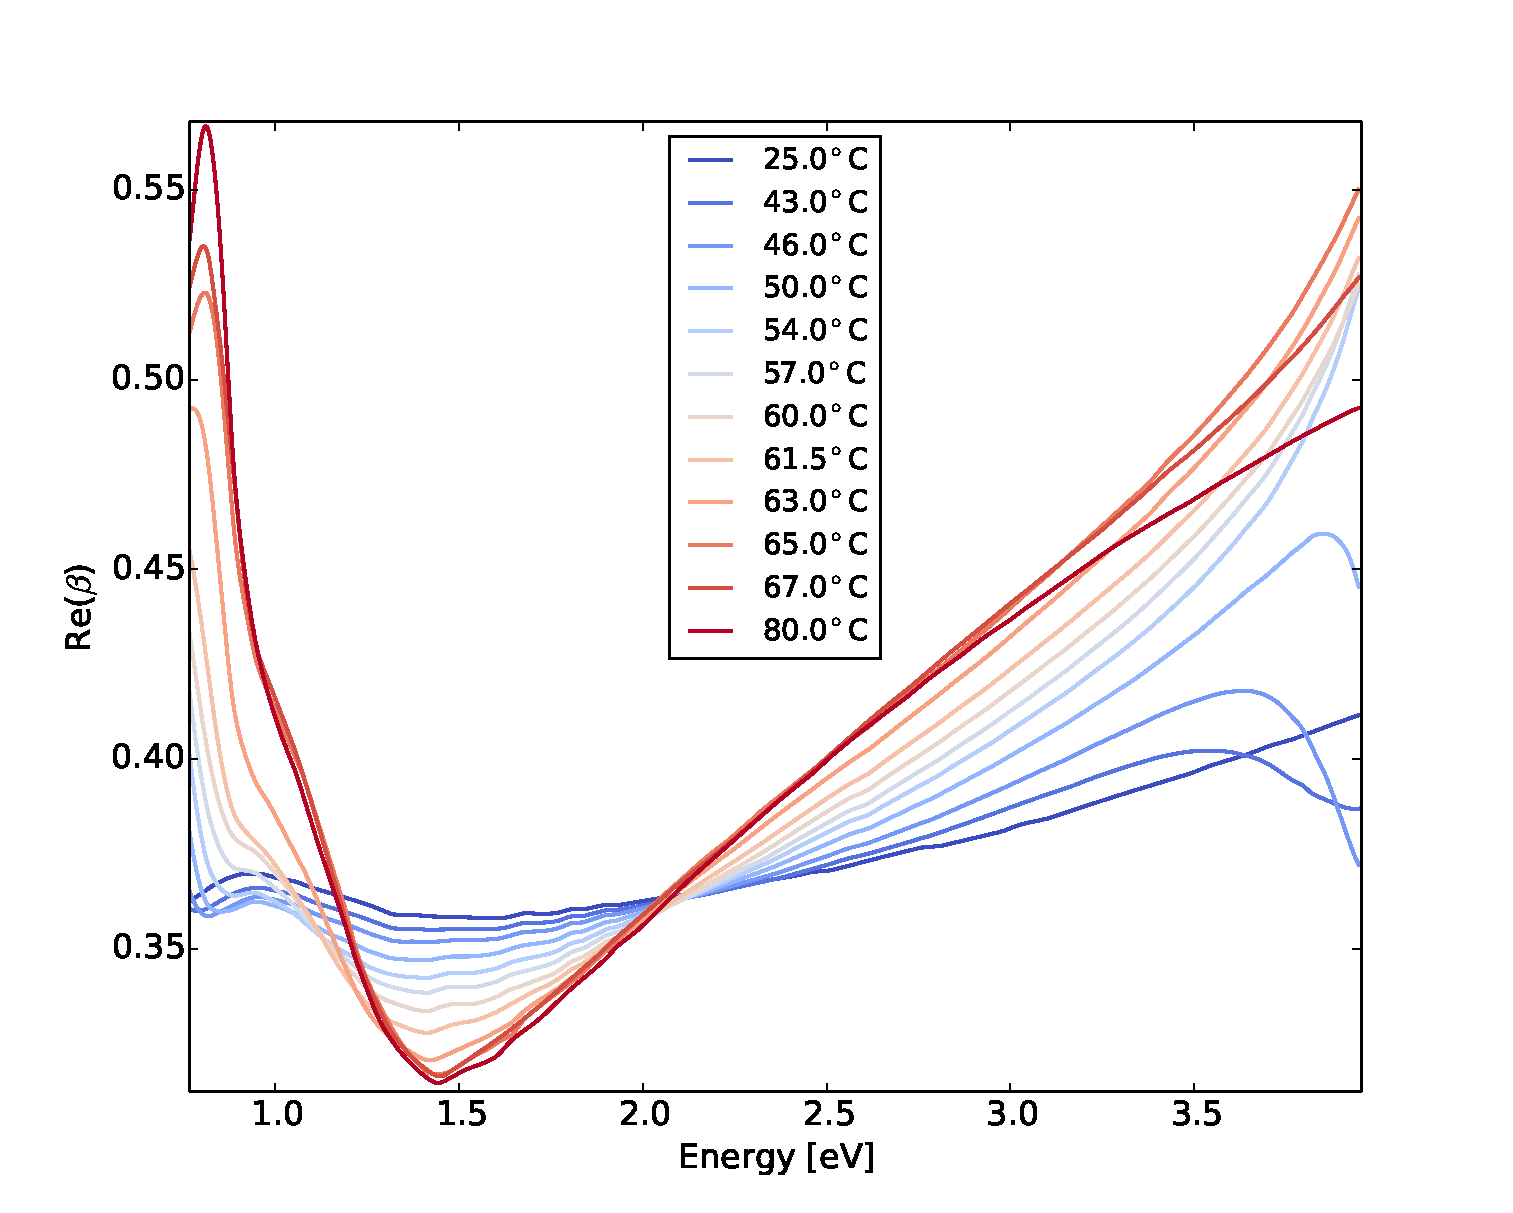
\includegraphics[width=\textwidth]{Results/Sim3/re_beta.pdf}
        \caption{}
        \label{fig:2}
    \end{subfigure}
    %\hfill
    \begin{subfigure}[b]{0.49\textwidth}
        \centering
        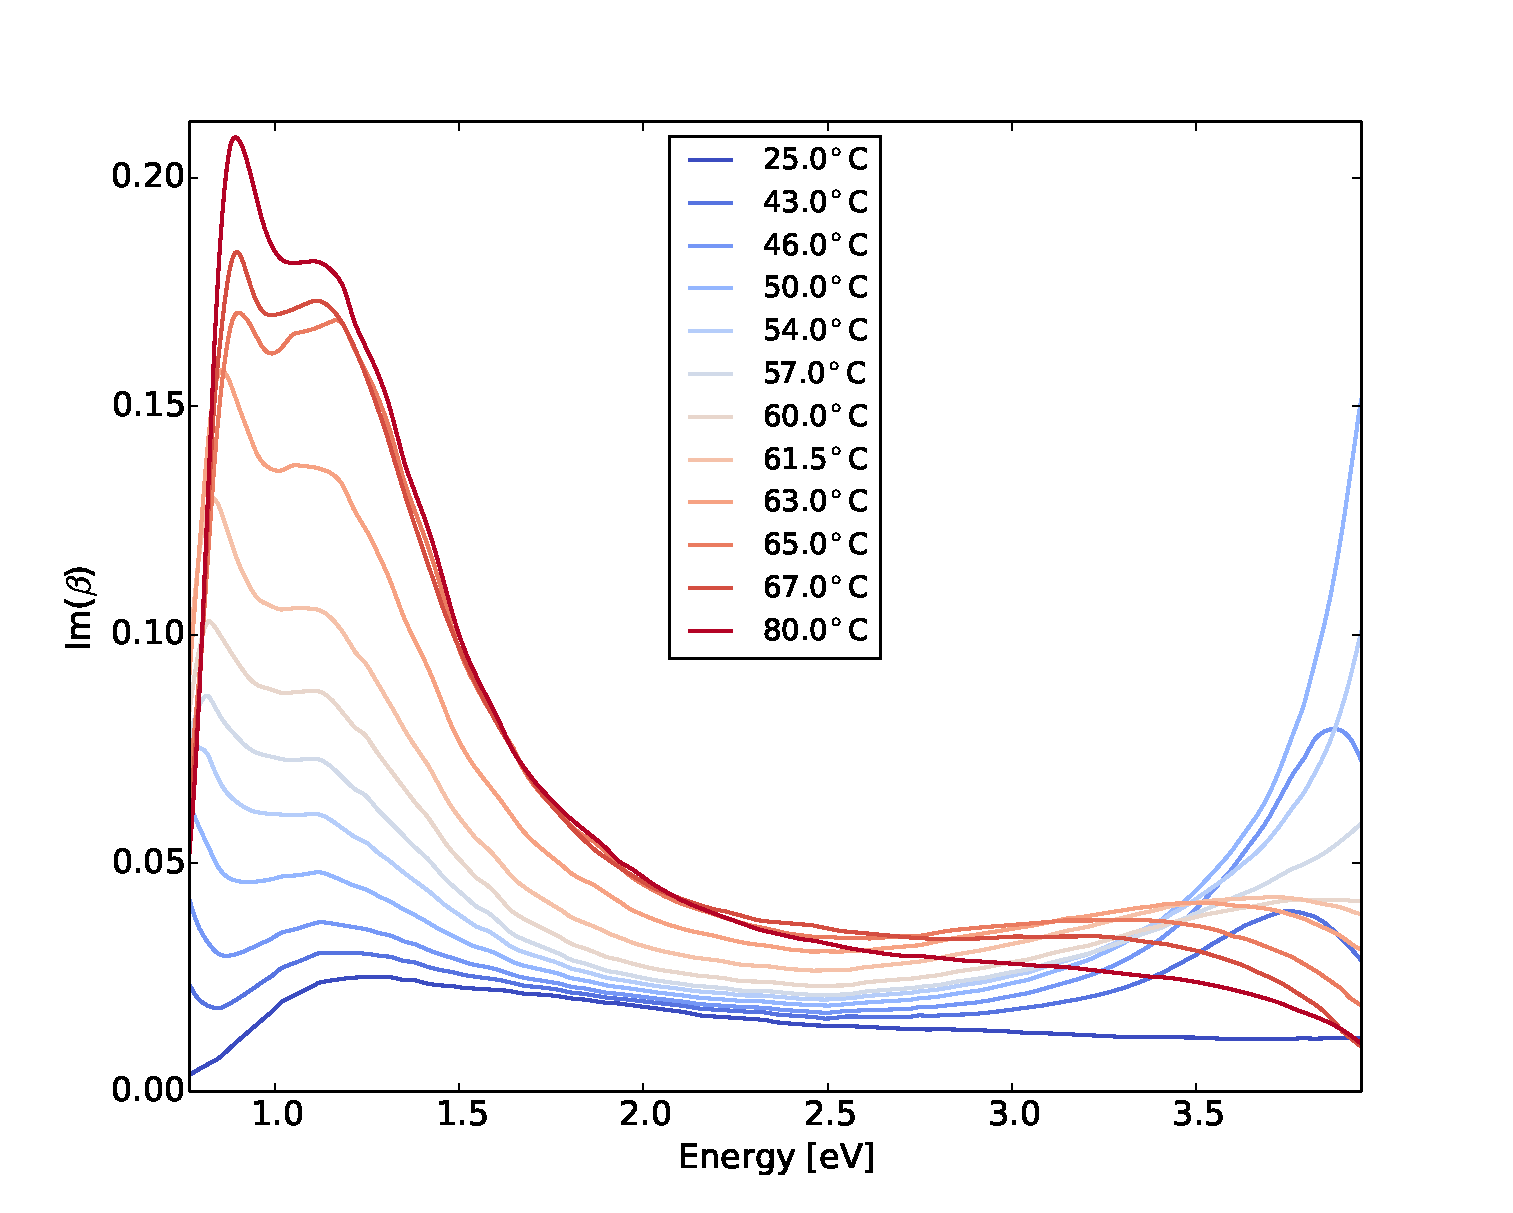
\includegraphics[width=\textwidth]{Results/Sim3/im_beta.pdf}
        \caption{}
        \label{fig:2}
    \end{subfigure}
    \caption{Relative reflectance $\Delta R/R$}
    \label{fig:}
\end{figure}
%

\subsection{Simulation 4; $R = 15$nm, s-polarized incident light}
%
\begin{figure}
    \centering
    \begin{subfigure}[b]{0.49\textwidth}
        \centering
        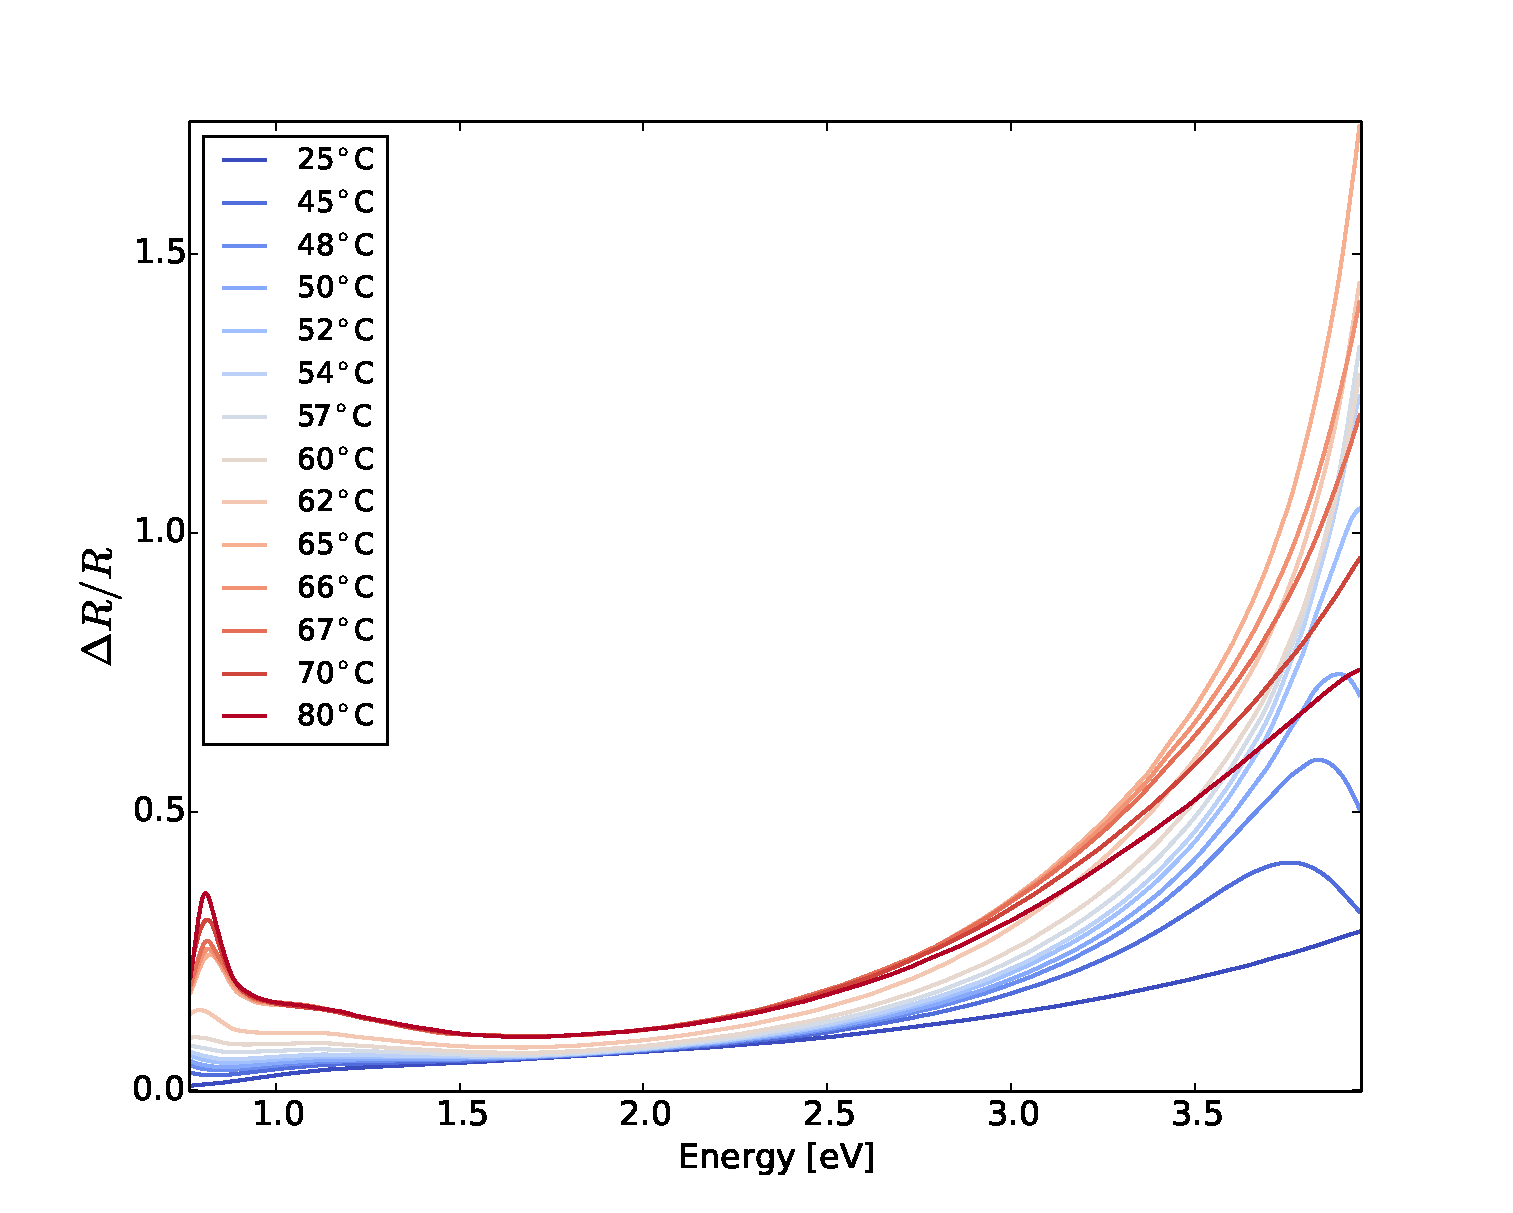
\includegraphics[width=\textwidth]{Results/Sim4/dR.pdf}
        \caption{}
        \label{fig:}
    \end{subfigure}
    %\hfill
    \begin{subfigure}[b]{0.49\textwidth}
        \centering
        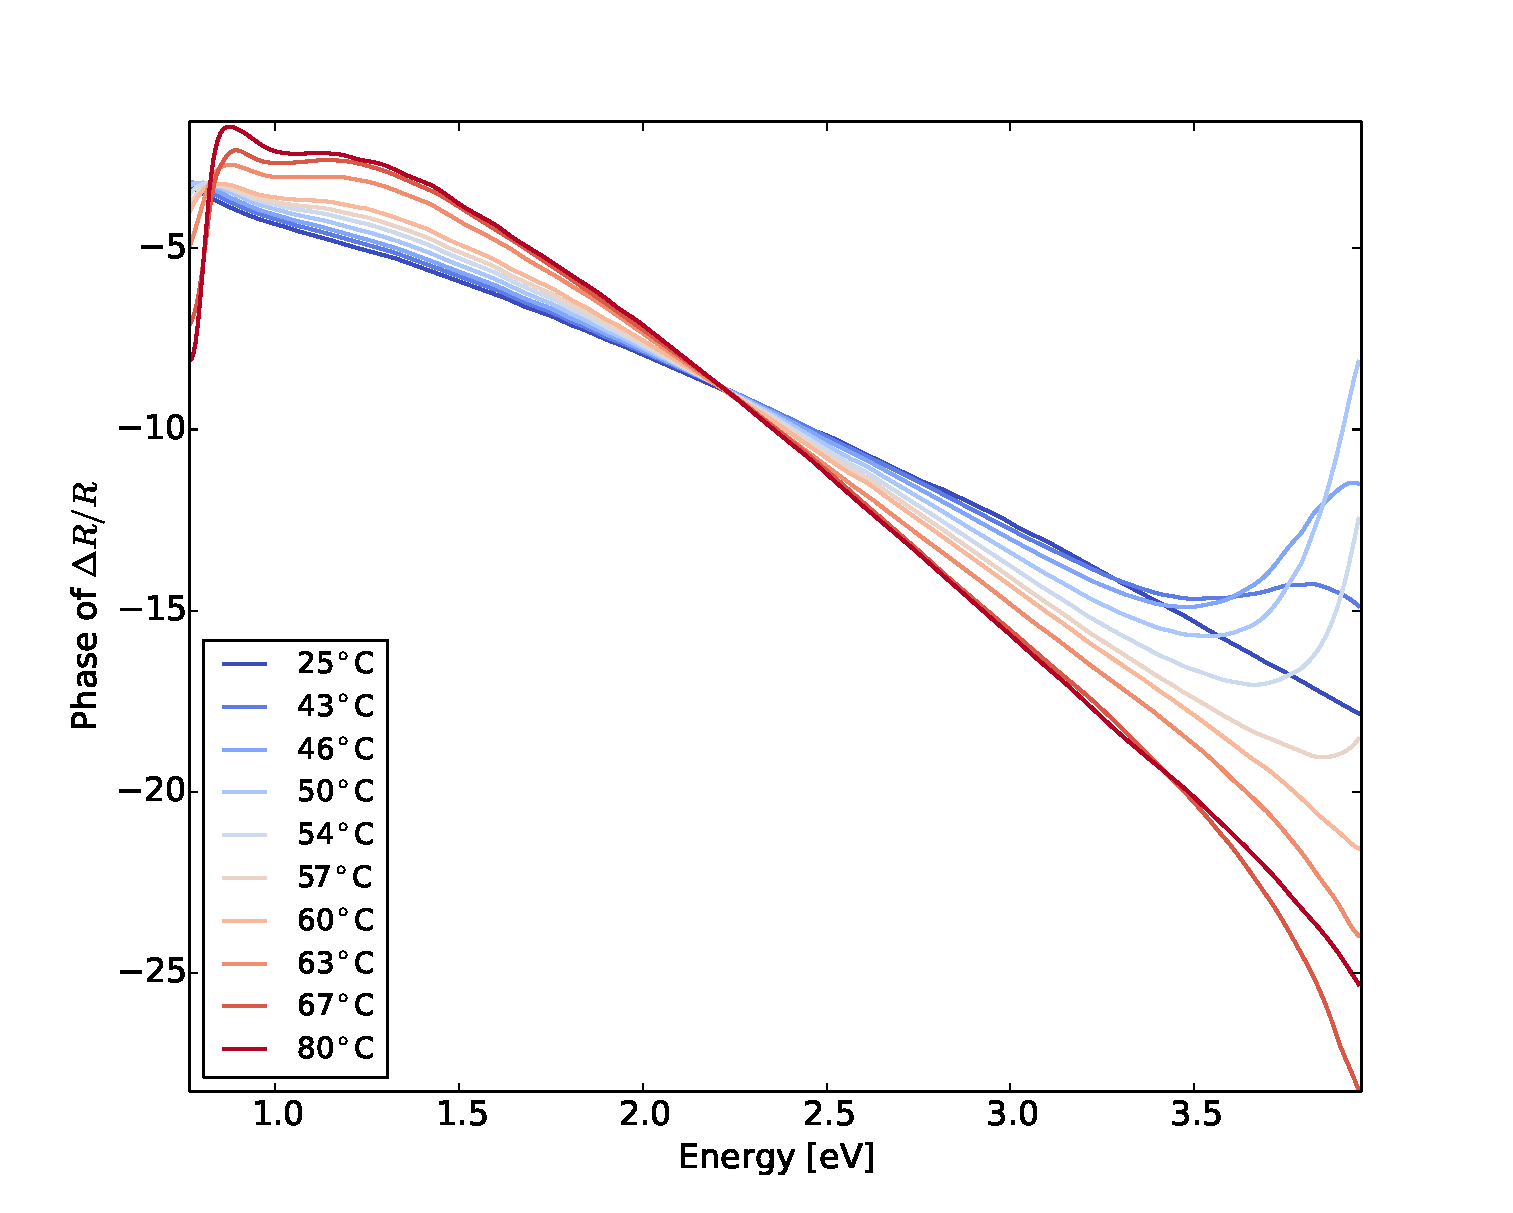
\includegraphics[width=\textwidth]{Results/Sim4/dRphase.pdf}
        \caption{}
        \label{fig:}
    \end{subfigure}
    \caption{Relative reflectance $\Delta R/R$}
    \label{fig:1}
\end{figure}
%
%
\begin{figure}
    \centering
    \begin{subfigure}[b]{0.49\textwidth}
        \centering
        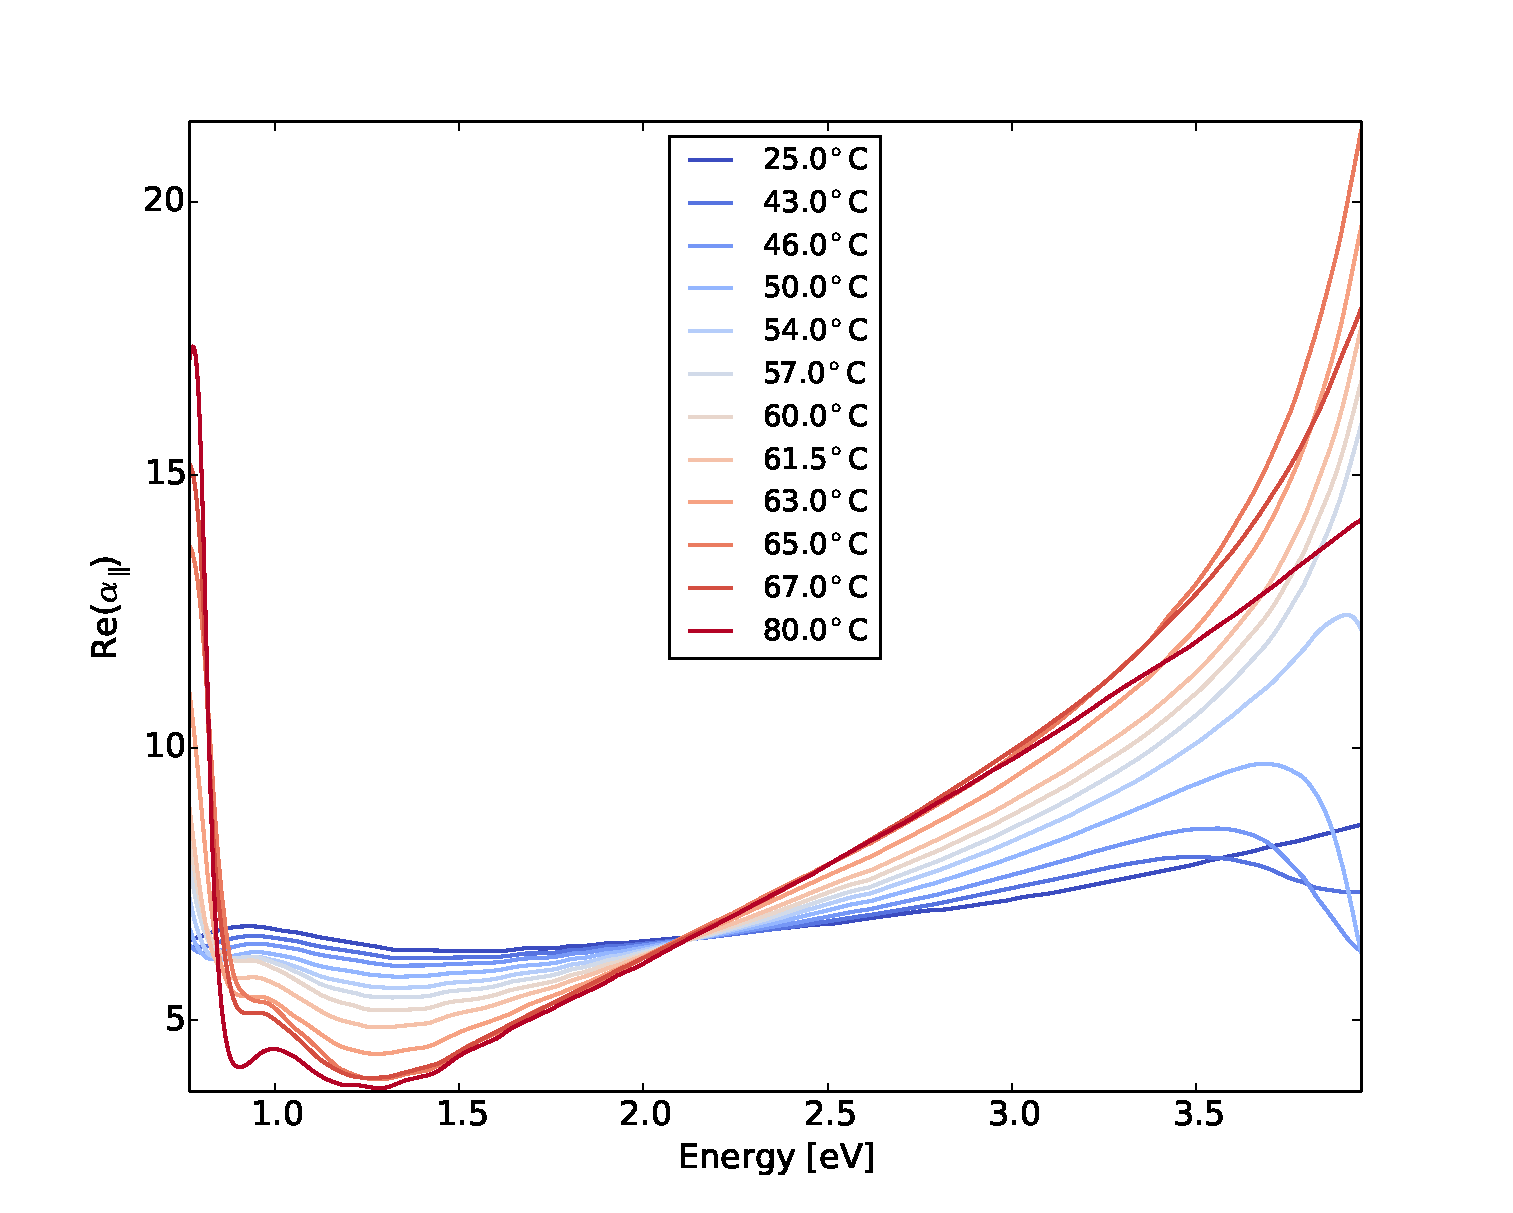
\includegraphics[width=\textwidth]{Results/Sim4/re_alpha_parallel.pdf}
        \caption{}
        \label{fig:2}
    \end{subfigure}
    %\hfill
    \begin{subfigure}[b]{0.49\textwidth}
        \centering
        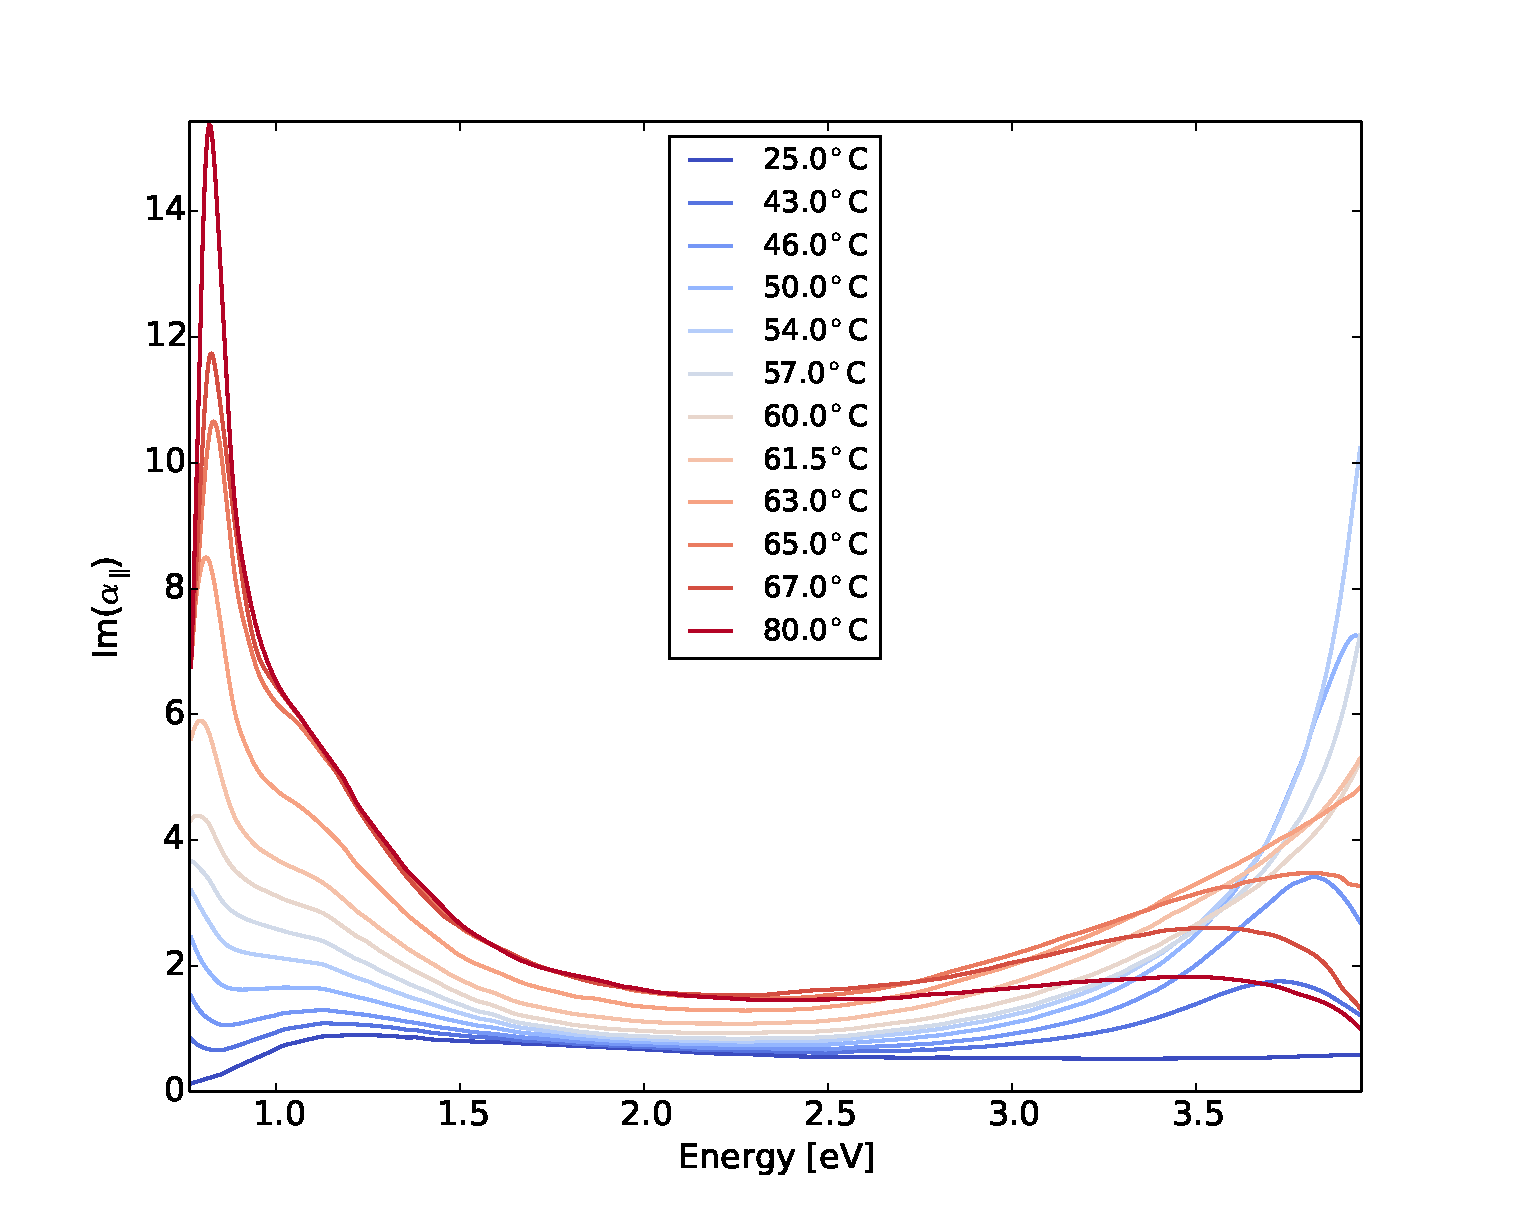
\includegraphics[width=\textwidth]{Results/Sim4/im_alpha_parallel.pdf}
        \caption{}
        \label{fig:2}
    \end{subfigure}
    %\hfill
    \begin{subfigure}[b]{0.49\textwidth}
        \centering
        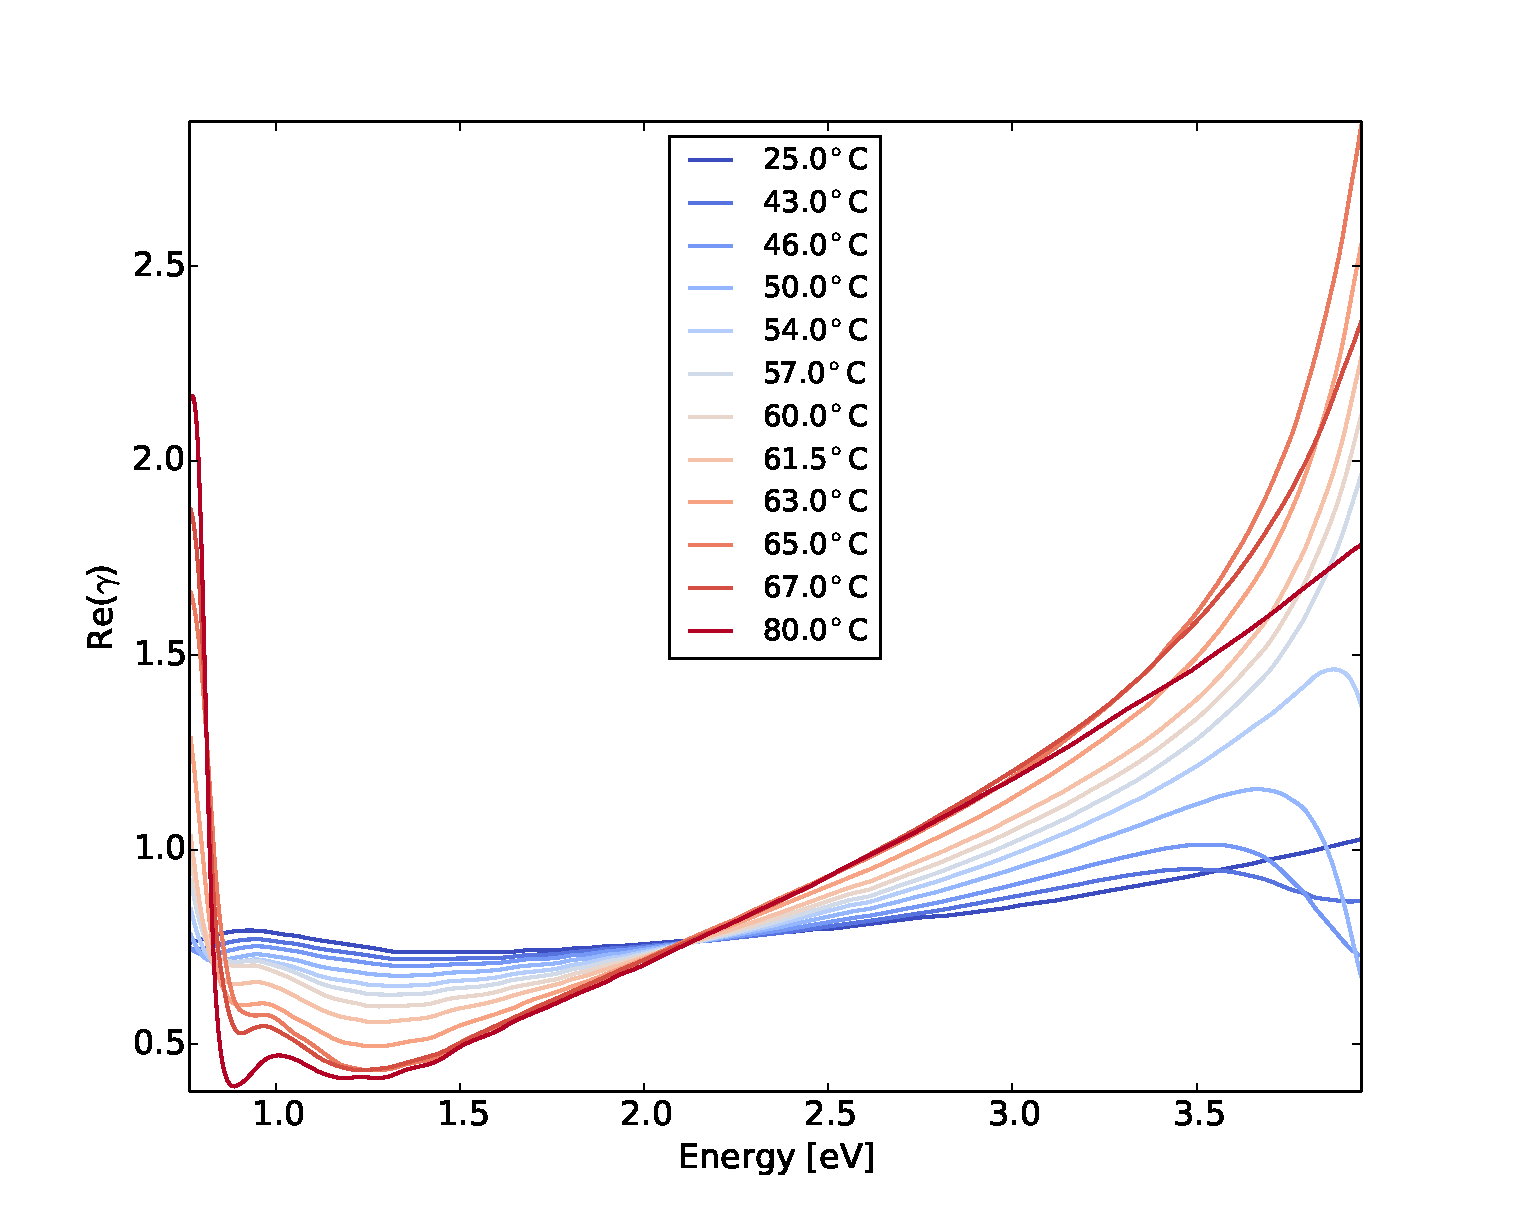
\includegraphics[width=\textwidth]{Results/Sim4/re_gamma.pdf}
        \caption{}
        \label{fig:2}
    \end{subfigure}
    %\hfill
    \begin{subfigure}[b]{0.49\textwidth}
        \centering
        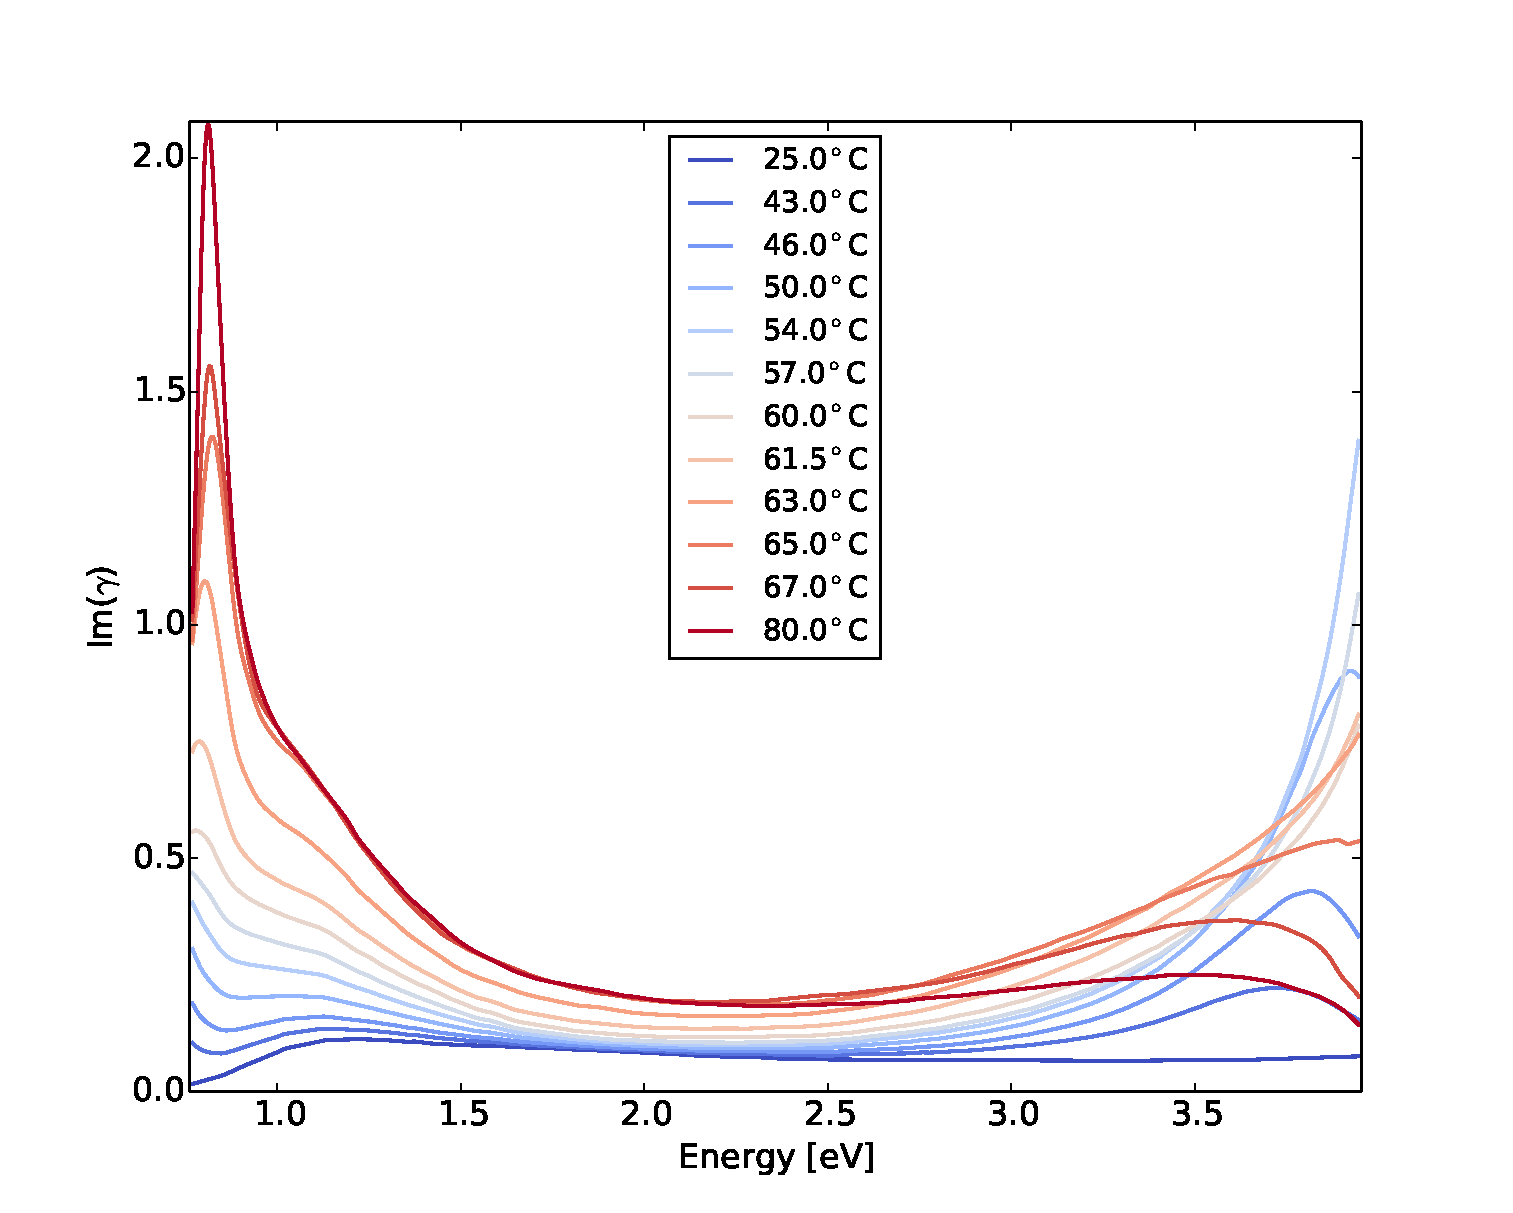
\includegraphics[width=\textwidth]{Results/Sim4/im_gamma.pdf}
        \caption{}
        \label{fig:2}
    \end{subfigure}
    \caption{Relative reflectance $\Delta R/R$}
    \label{fig:}
\end{figure}
%
%
\begin{figure}
    \centering
    \begin{subfigure}[b]{0.49\textwidth}
        \centering
        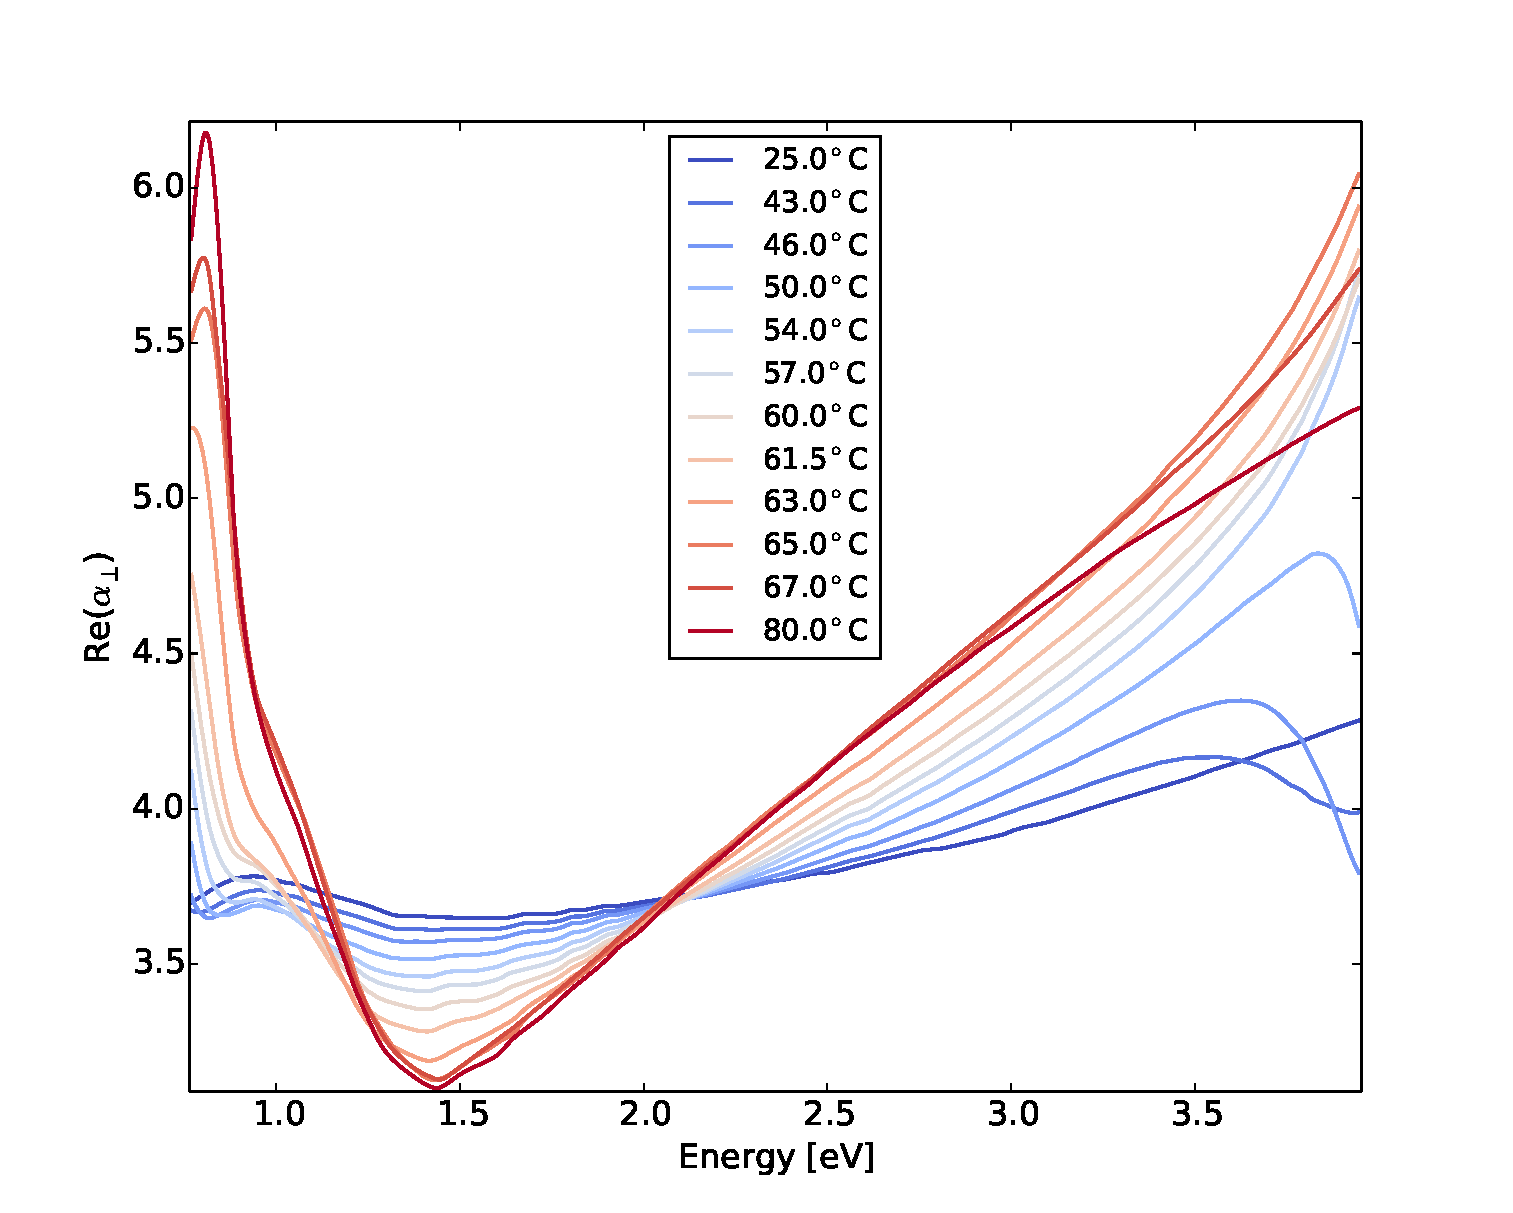
\includegraphics[width=\textwidth]{Results/Sim4/re_alpha_perp.pdf}
        \caption{}
        \label{fig:}
    \end{subfigure}
    %\hfill
    \begin{subfigure}[b]{0.49\textwidth}
        \centering
        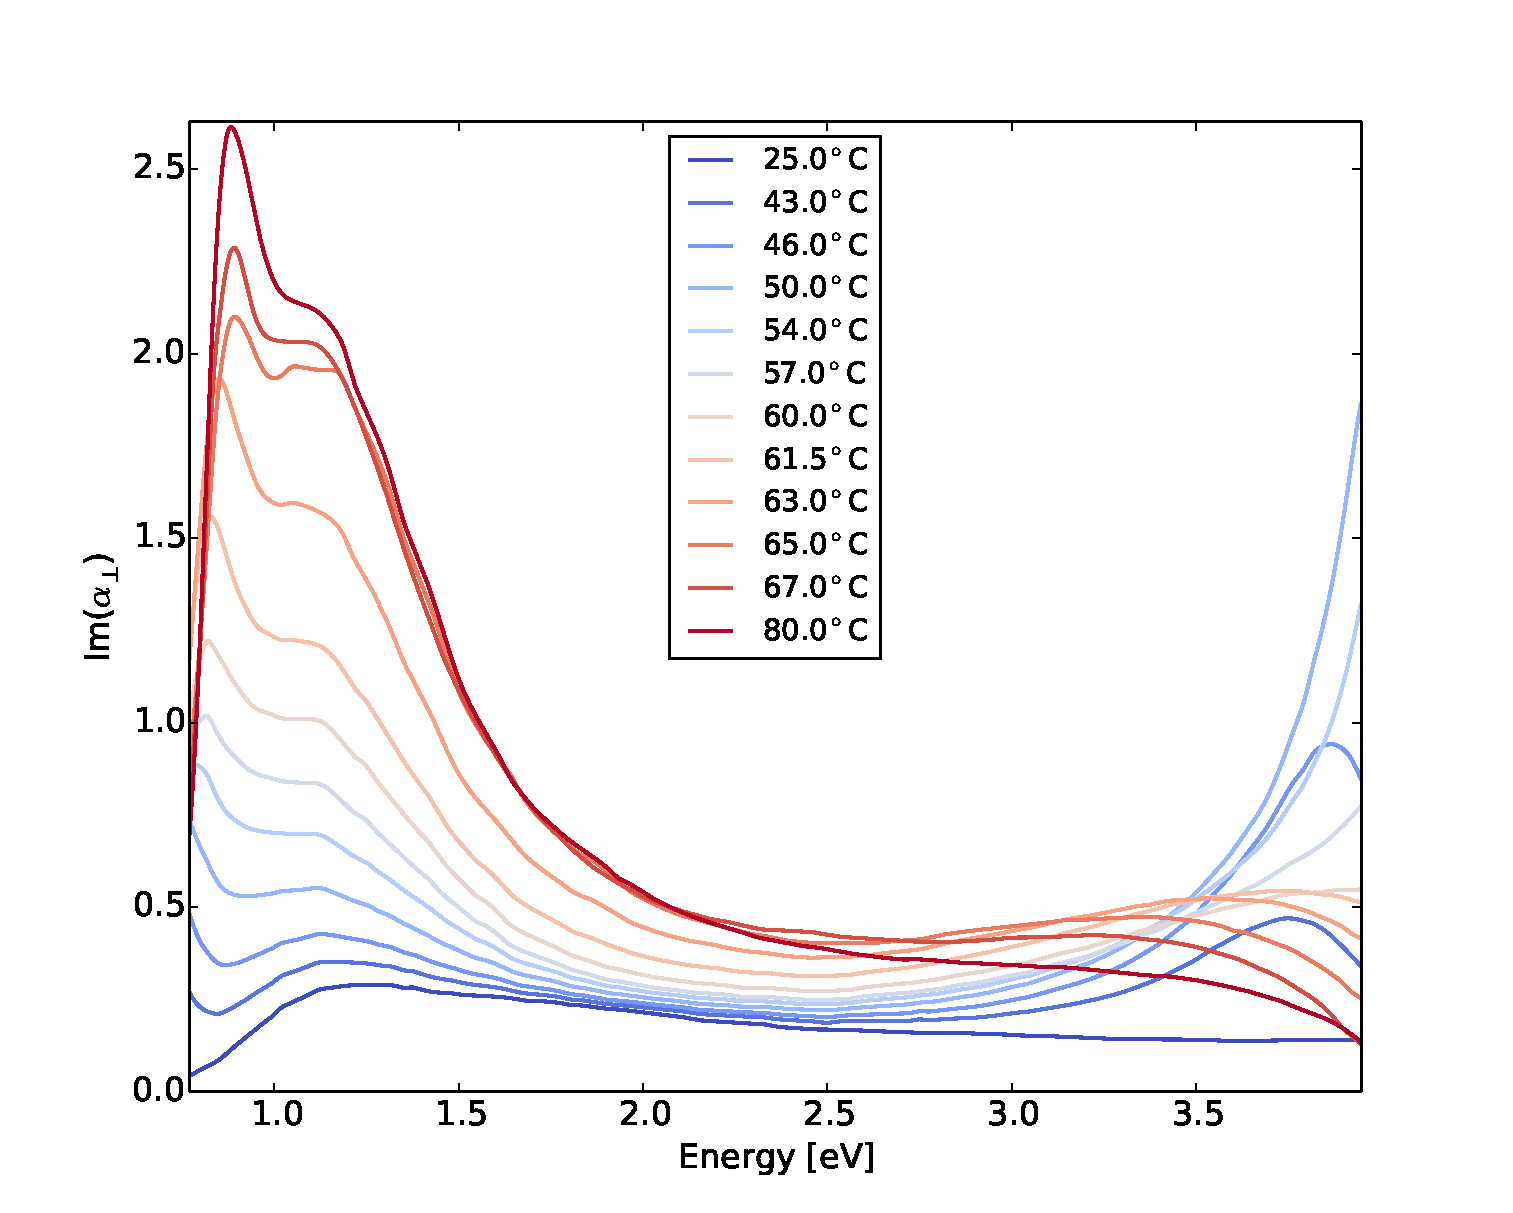
\includegraphics[width=\textwidth]{Results/Sim4/im_alpha_perp.pdf}
        \caption{}
        \label{fig:}
    \end{subfigure}
    %\hfill
    \begin{subfigure}[b]{0.49\textwidth}
        \centering
        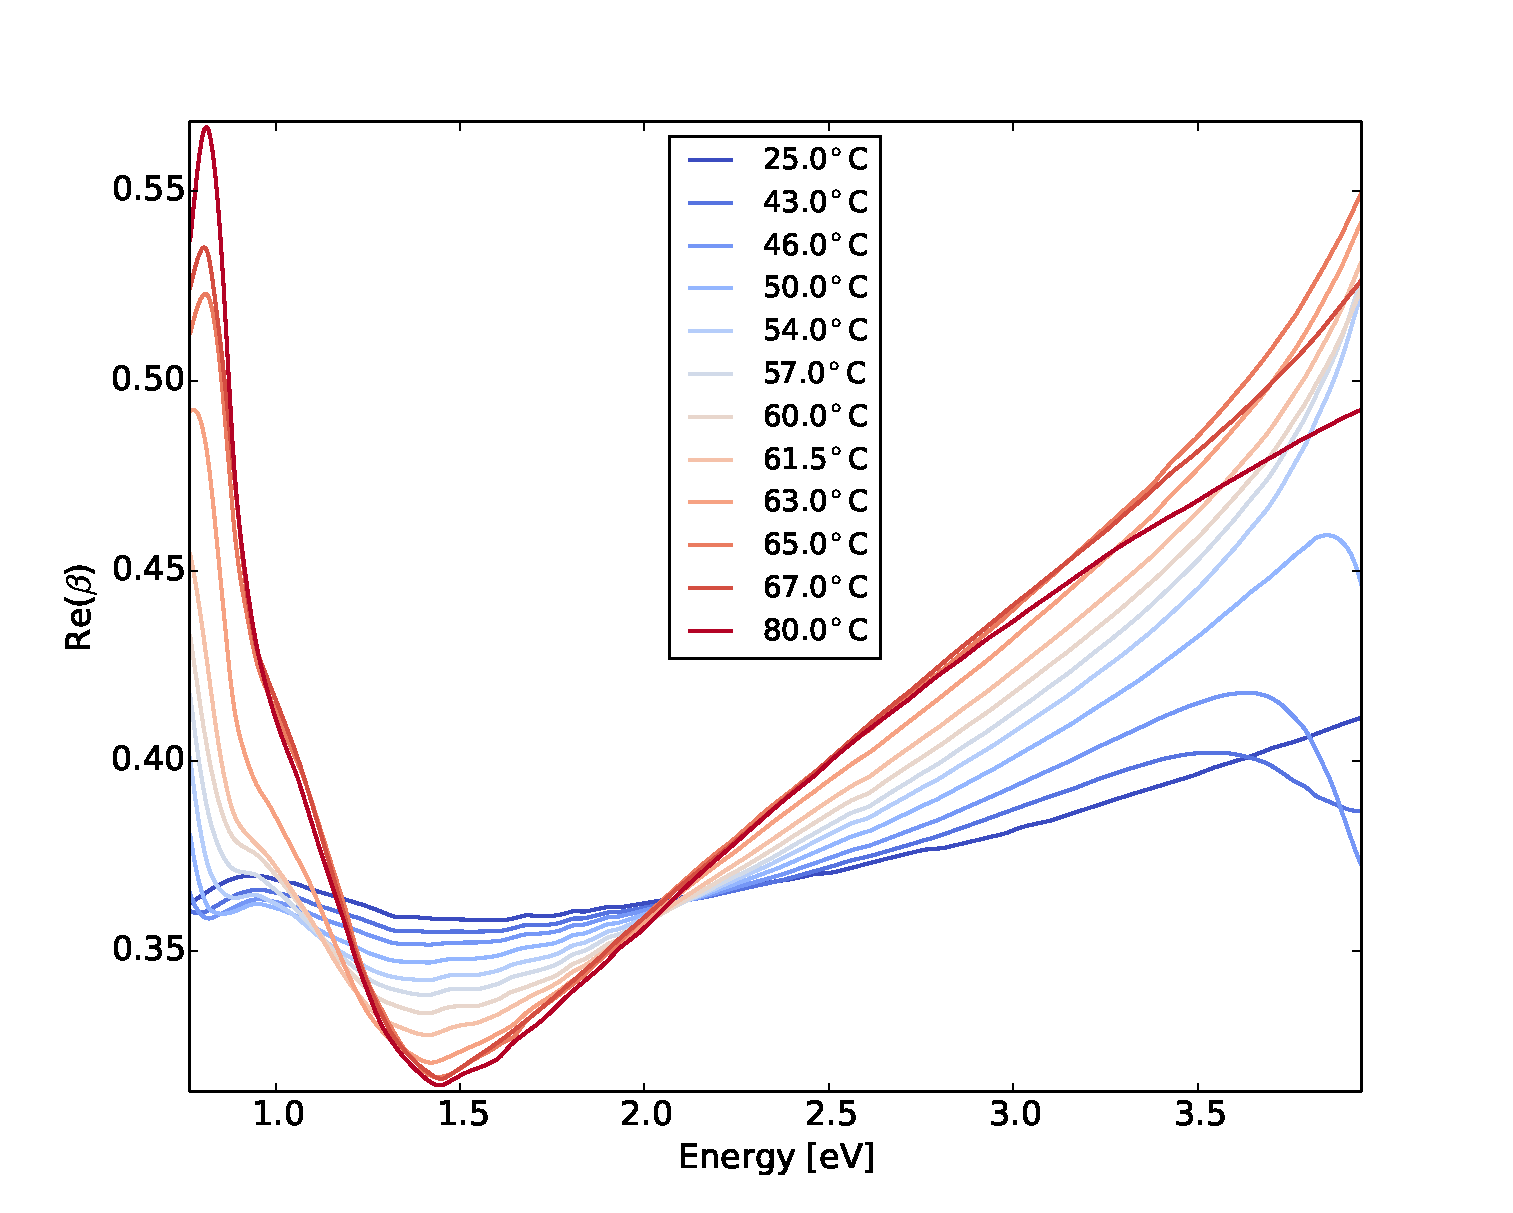
\includegraphics[width=\textwidth]{Results/Sim4/re_beta.pdf}
        \caption{}
        \label{fig:2}
    \end{subfigure}
    %\hfill
    \begin{subfigure}[b]{0.49\textwidth}
        \centering
        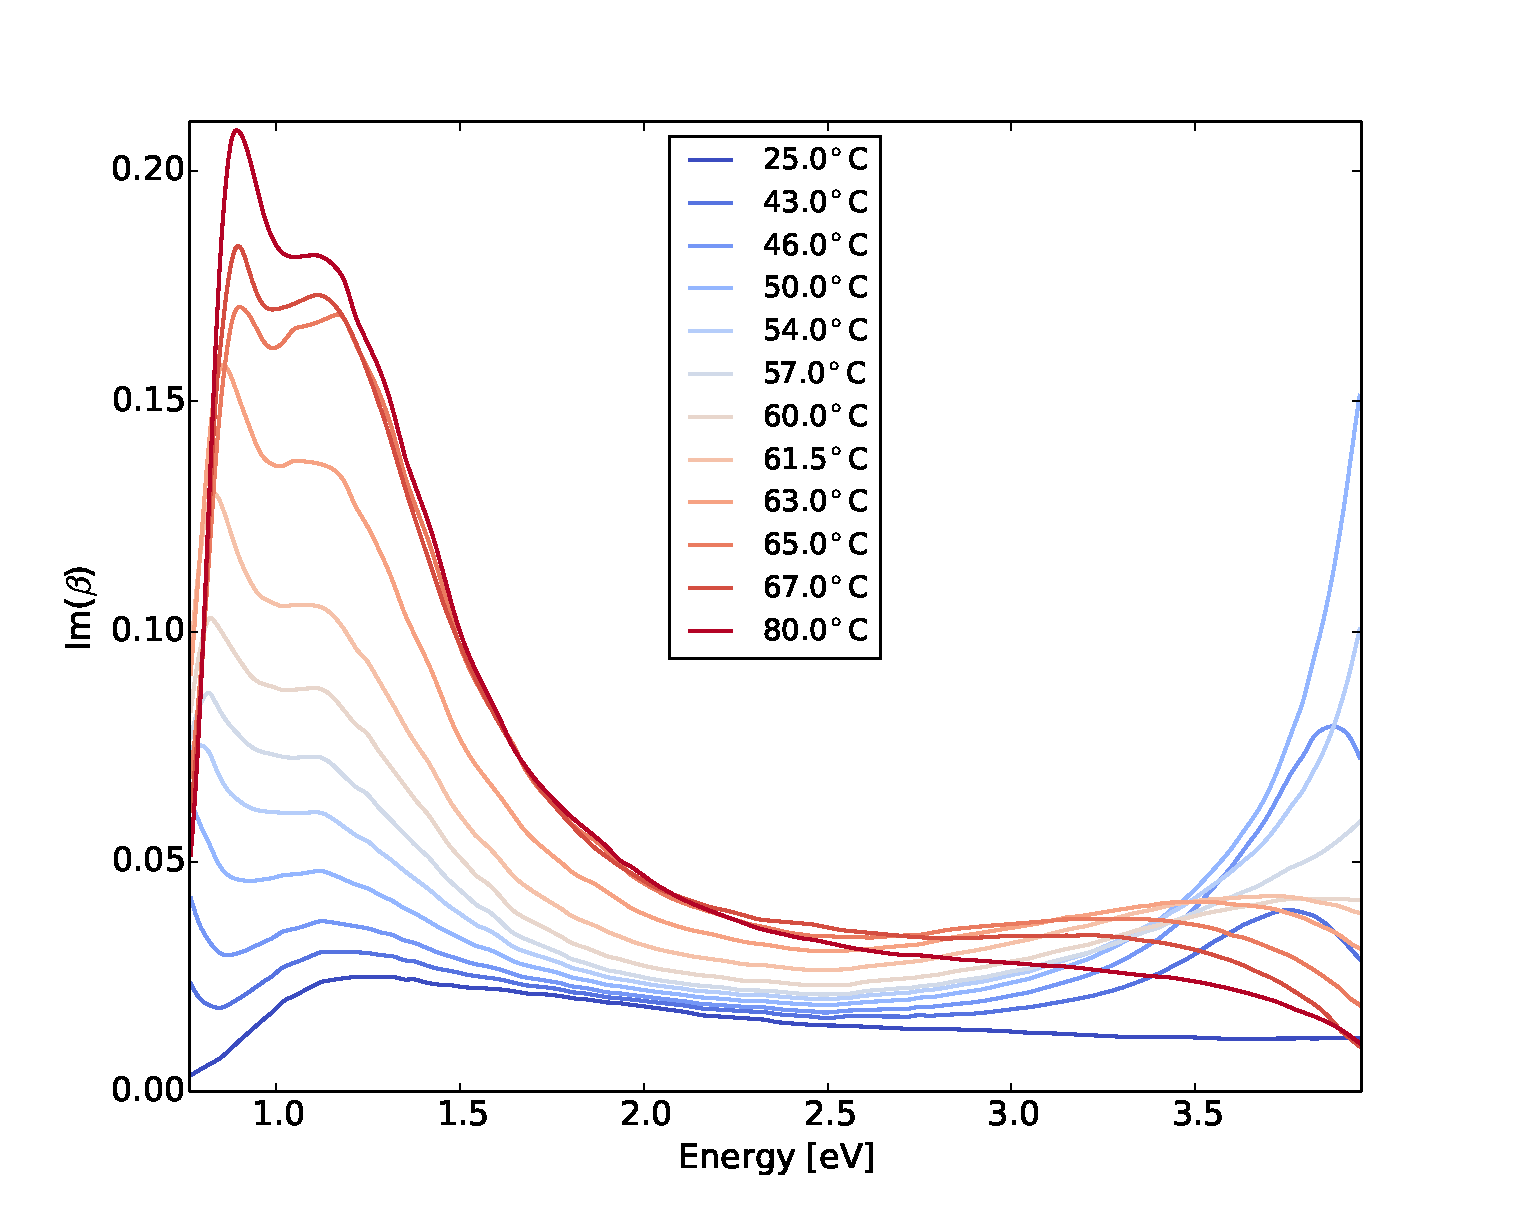
\includegraphics[width=\textwidth]{Results/Sim4/im_beta.pdf}
        \caption{}
        \label{fig:2}
    \end{subfigure}
    \caption{Relative reflectance $\Delta R/R$}
    \label{fig:}
\end{figure}
%




\begin{figure}
    \centering
    \begin{subfigure}[b]{0.3\textwidth}
        \centering
        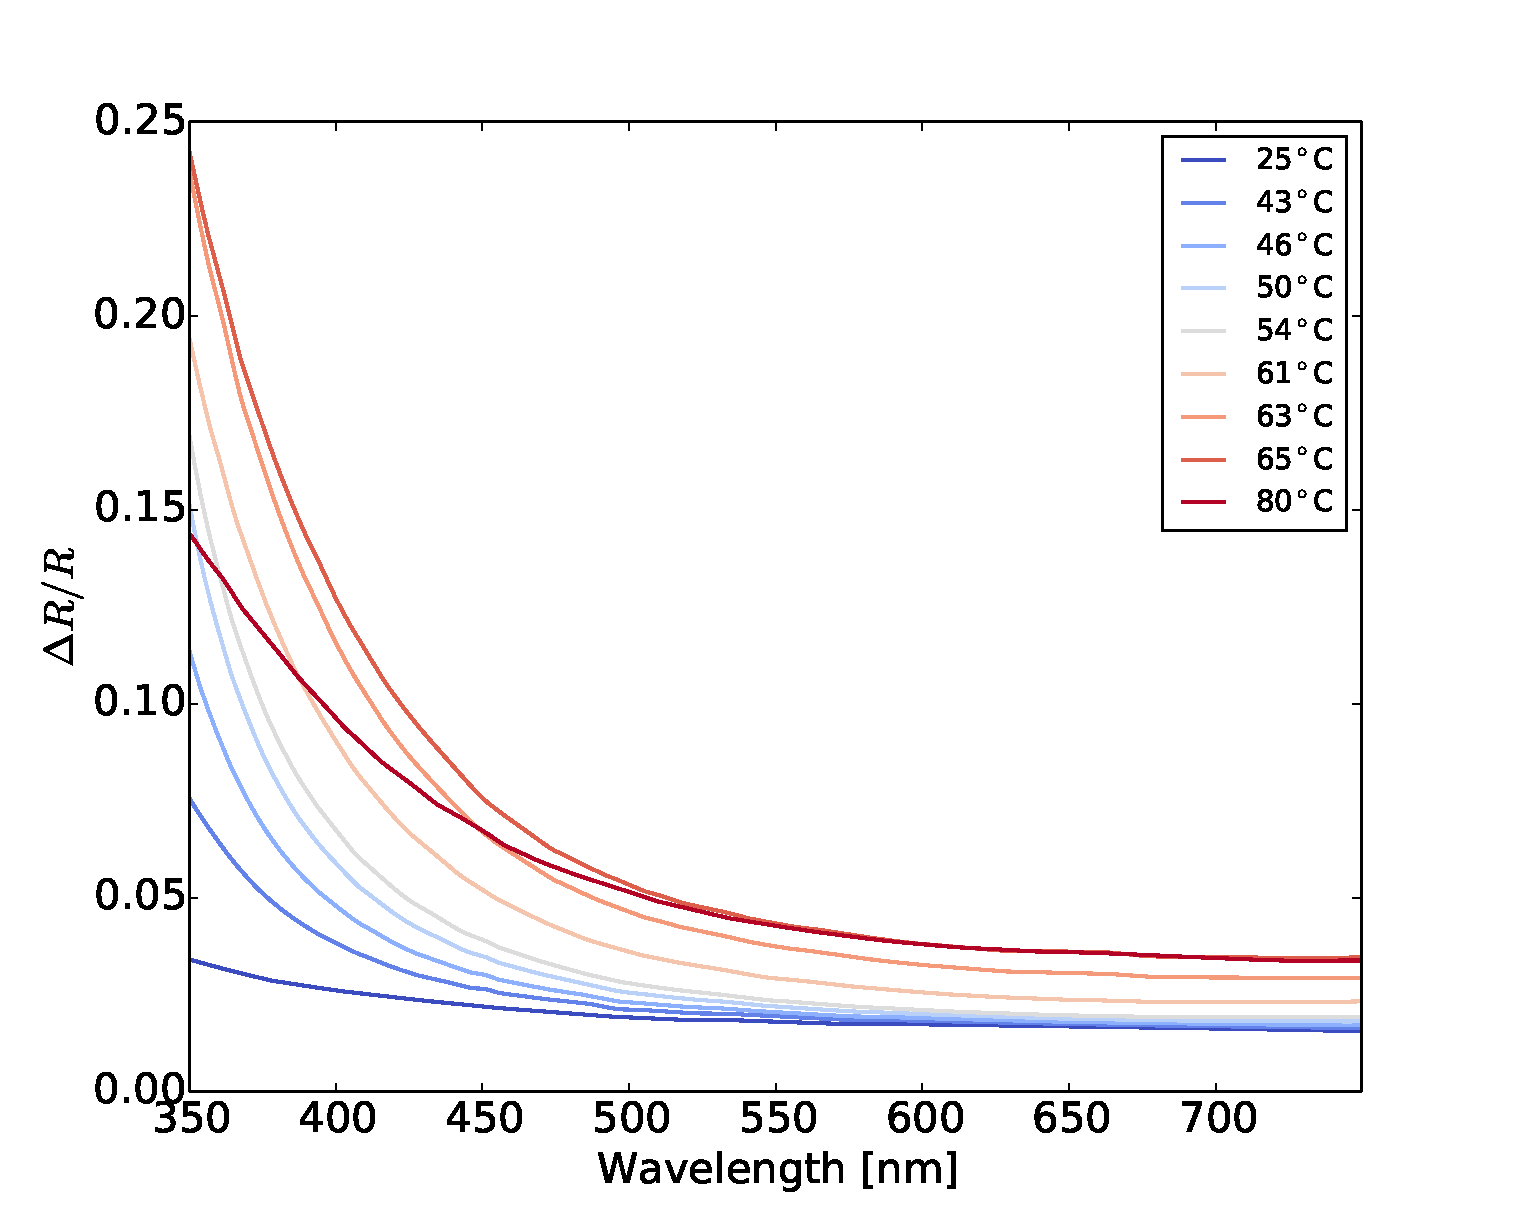
\includegraphics[width=\textwidth]{Results/Sim1/dR_visible.pdf}
        \caption{}
        %\label{fig:y equals x}
    \end{subfigure}
    %\hfill
    \begin{subfigure}[b]{0.3\textwidth}
        \centering
        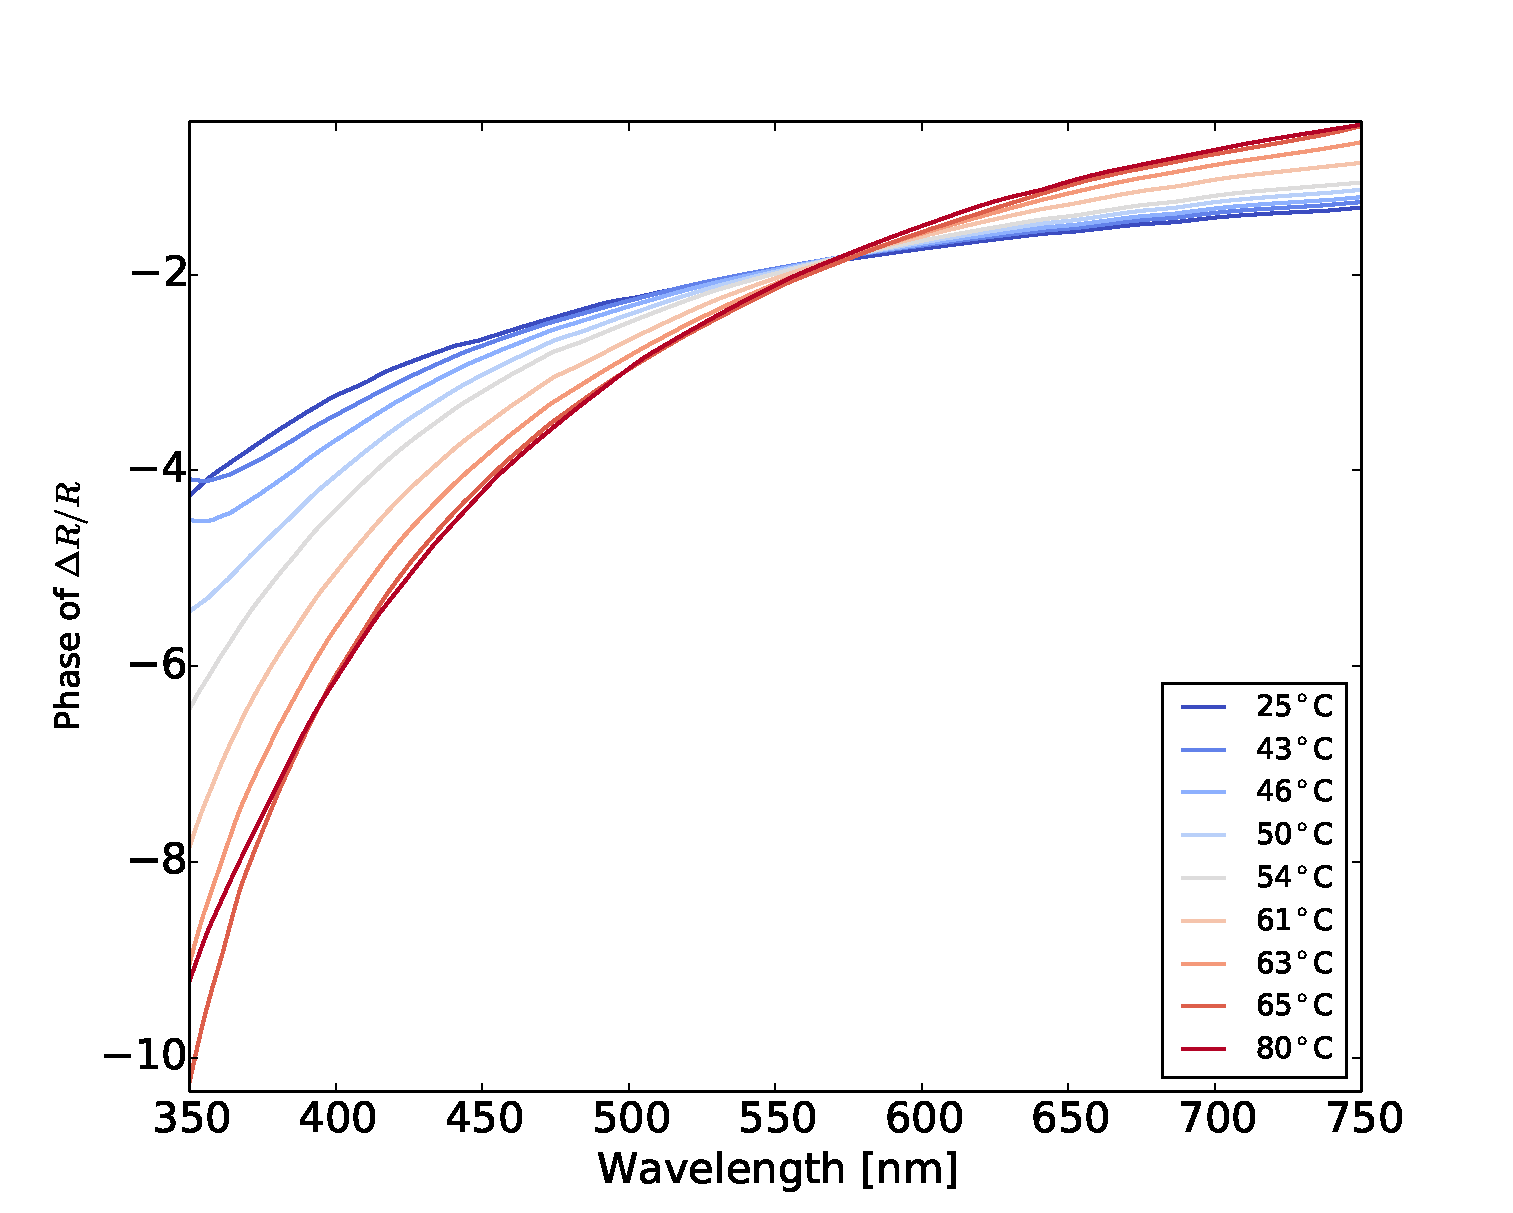
\includegraphics[width=\textwidth]{Results/Sim1/dRphase_visible.pdf}
        \caption{}
        %\label{fig:five over x}
    \end{subfigure}
    %\hfill
    \begin{subfigure}[b]{0.3\textwidth}
        \centering
        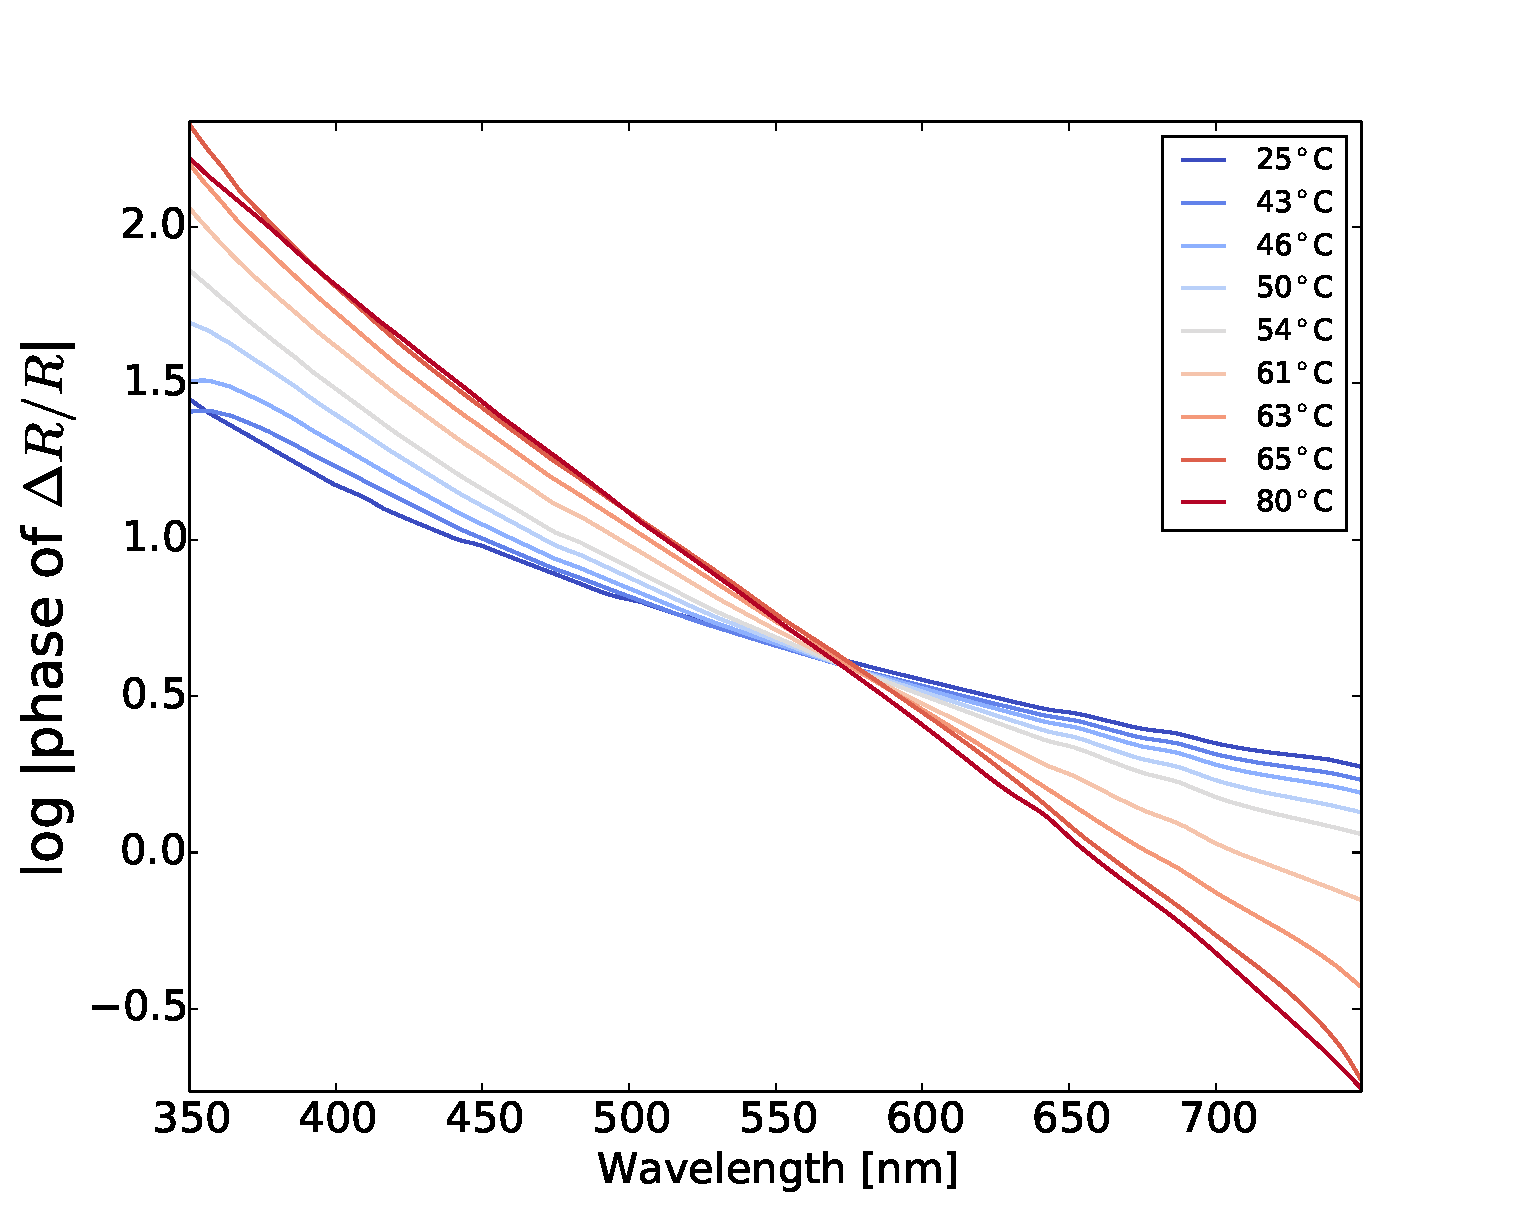
\includegraphics[width=\textwidth]{Results/Sim1/dRphase_visible_log.pdf}
        \caption{}
        %\label{fig:three sin x}
    \end{subfigure}
    \caption{R = 10nm, p-pol}
    %\label{fig:three graphs}
\end{figure}
%
\begin{figure}
    \centering
    \begin{subfigure}[b]{0.3\textwidth}
        \centering
        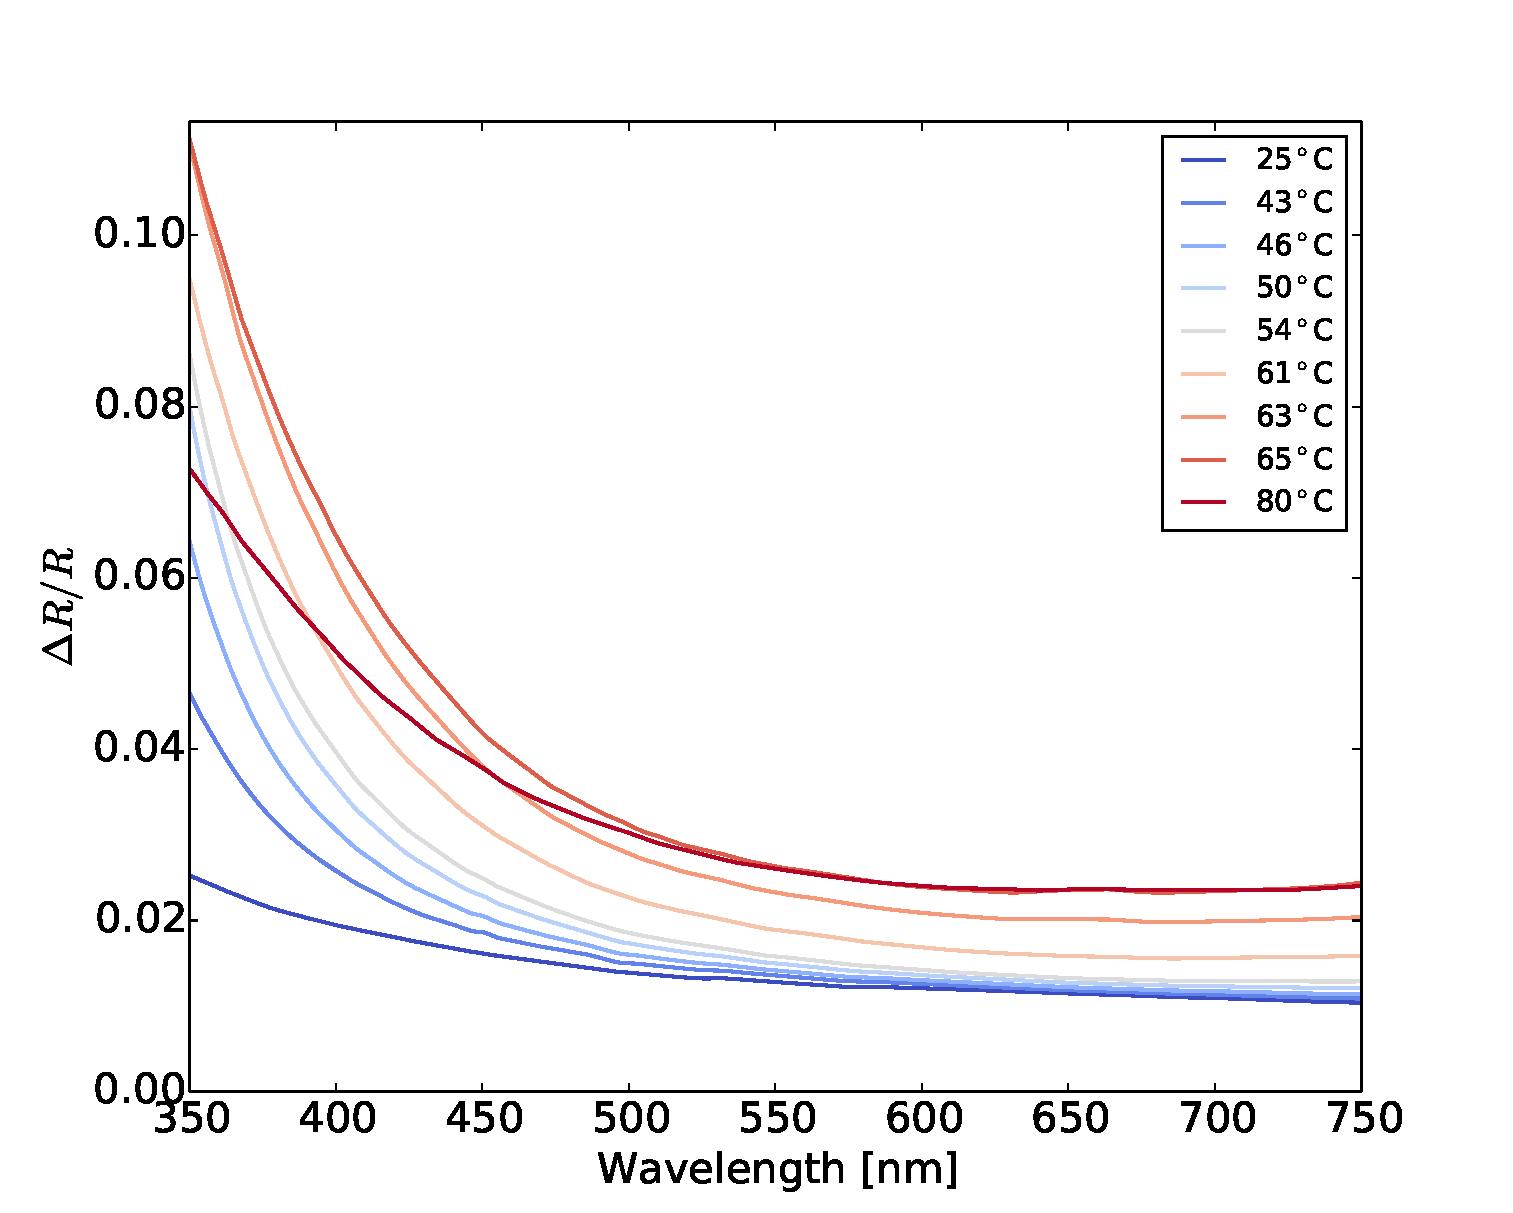
\includegraphics[width=\textwidth]{Results/Sim2/dR_visible.pdf}
        \caption{}
        %\label{fig:y equals x}
    \end{subfigure}
    %\hfill
    \begin{subfigure}[b]{0.3\textwidth}
        \centering
        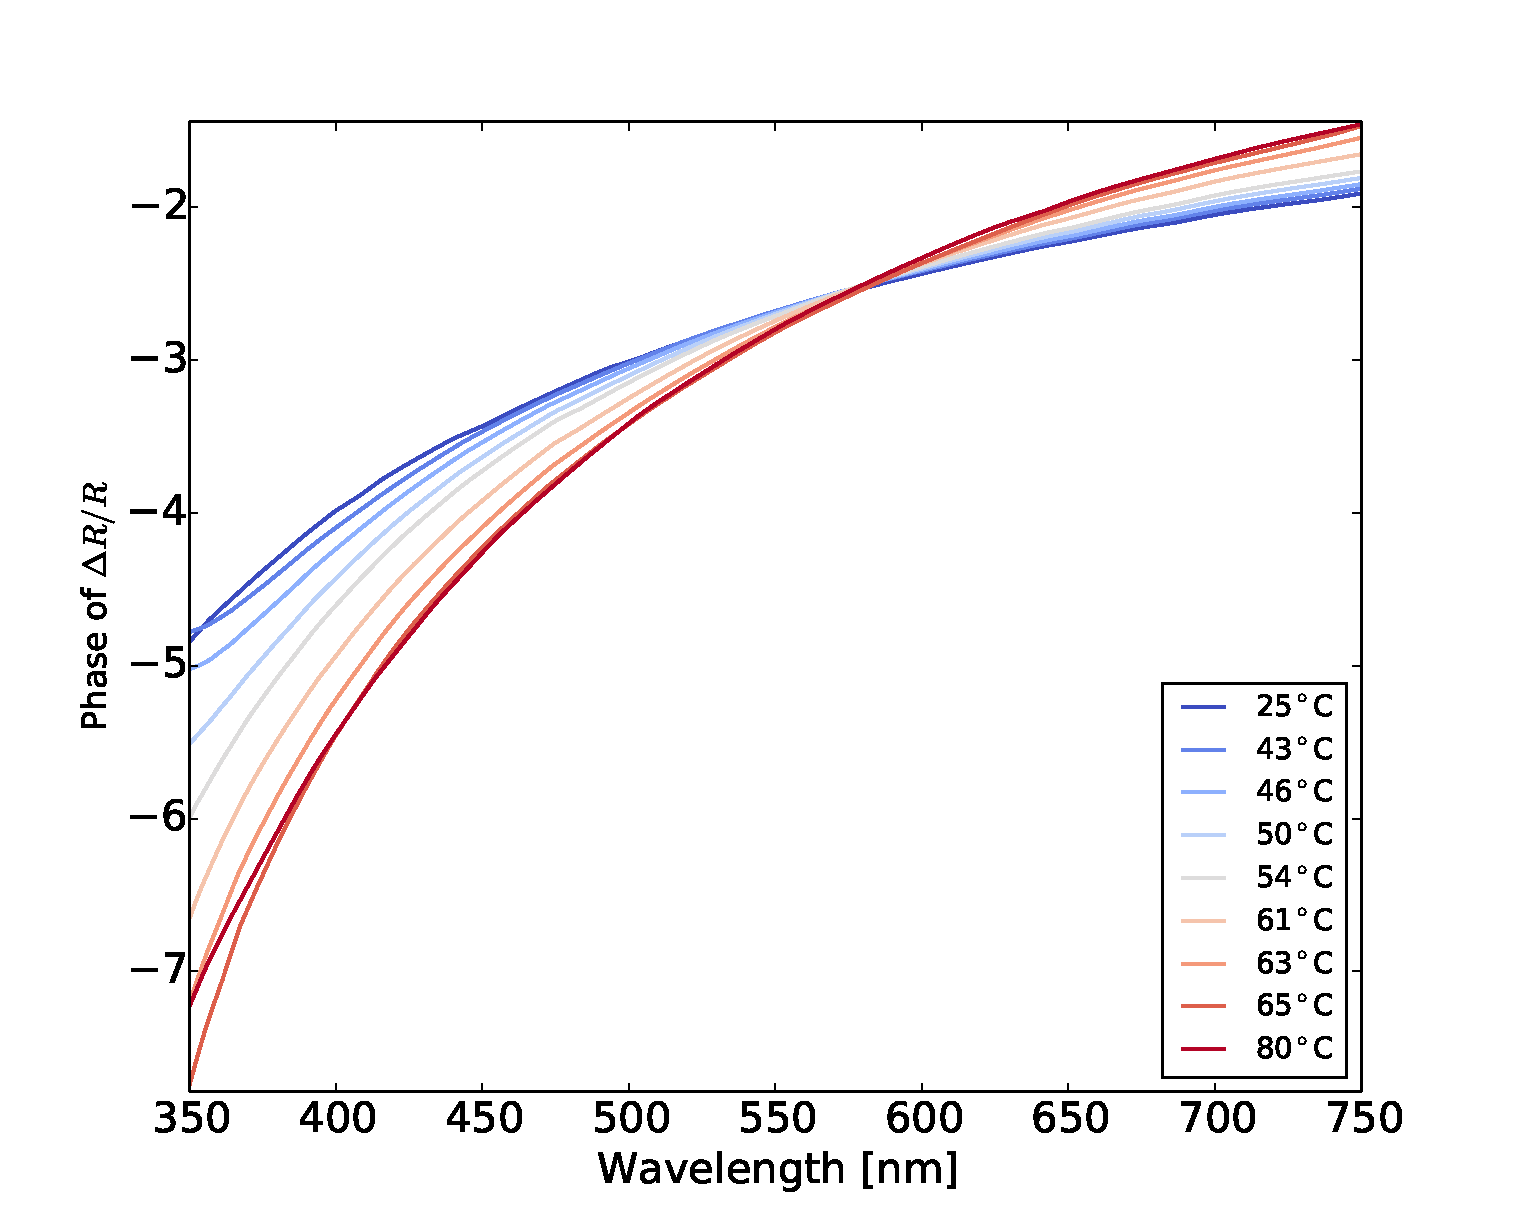
\includegraphics[width=\textwidth]{Results/Sim2/dRphase_visible.pdf}
        \caption{}
        %\label{fig:five over x}
    \end{subfigure}
    %\hfill
    \begin{subfigure}[b]{0.3\textwidth}
        \centering
        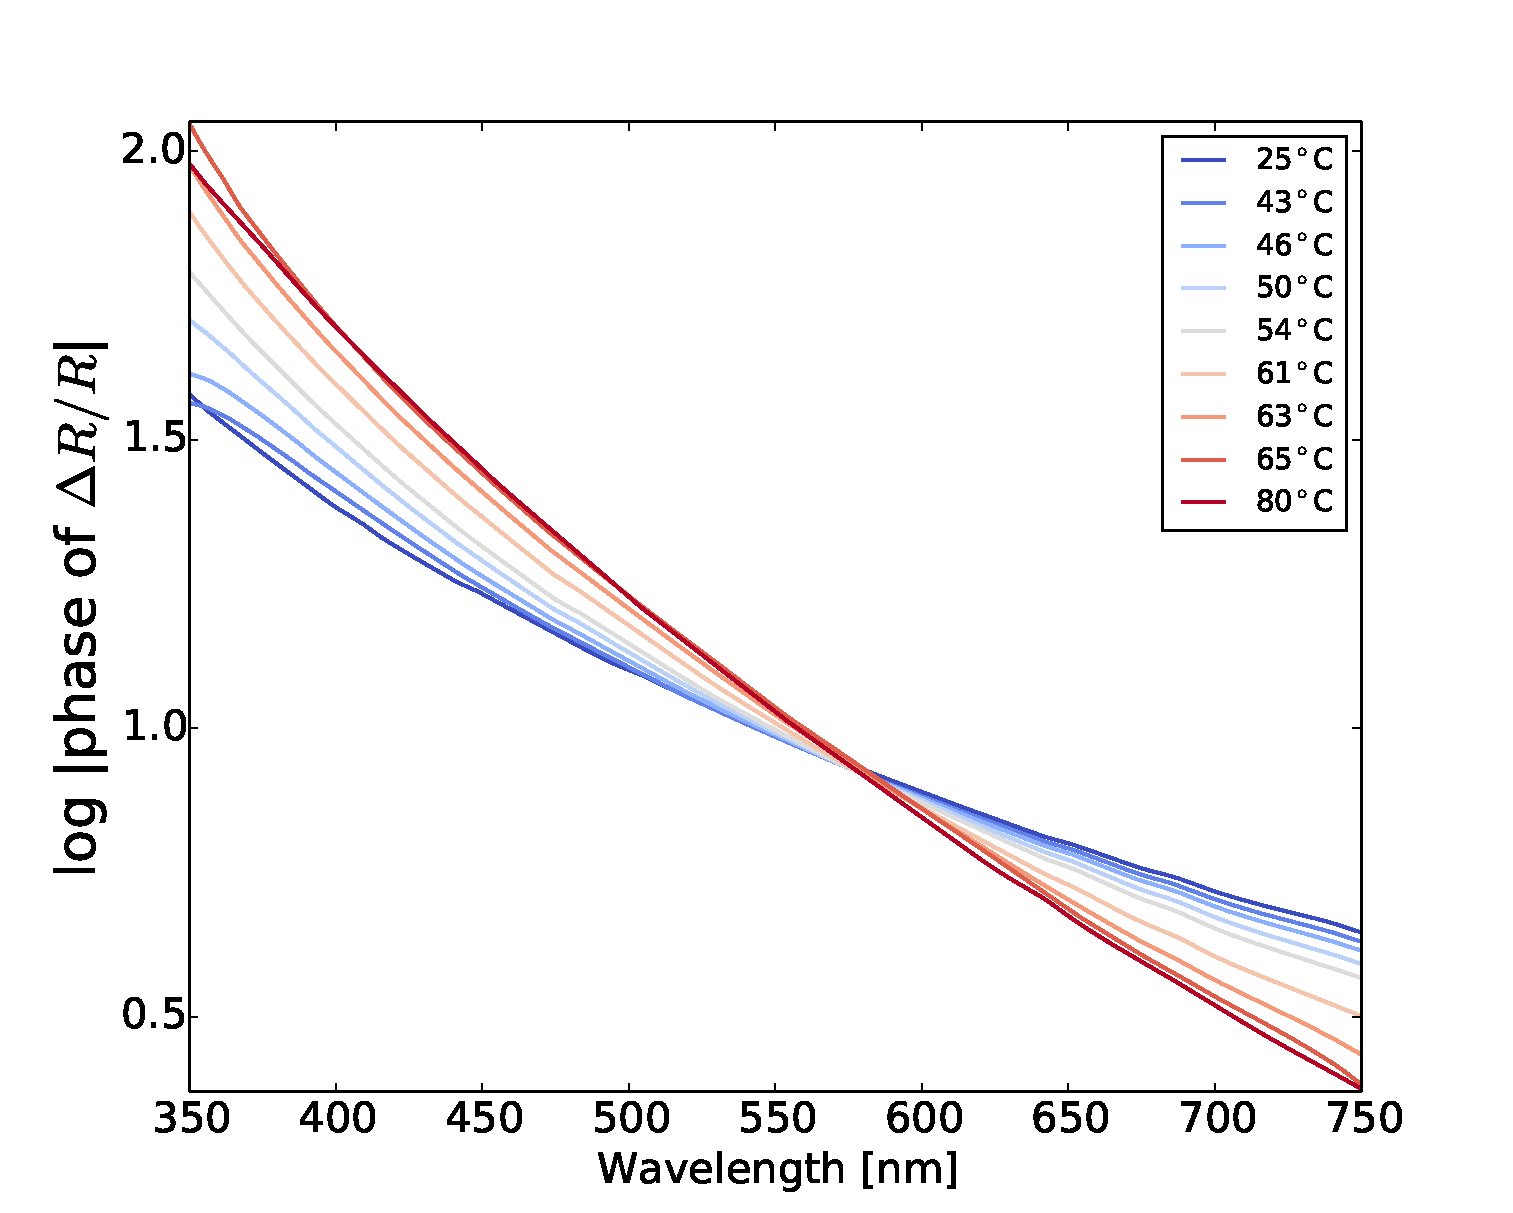
\includegraphics[width=\textwidth]{Results/Sim2/dRphase_visible_log.pdf}
        \caption{}
        %\label{fig:three sin x}
    \end{subfigure}
    \caption{R = 10nm, s-pol}
    %\label{fig:three graphs}
\end{figure}
%
\begin{figure}
    \centering
    \begin{subfigure}[b]{0.3\textwidth}
        \centering
        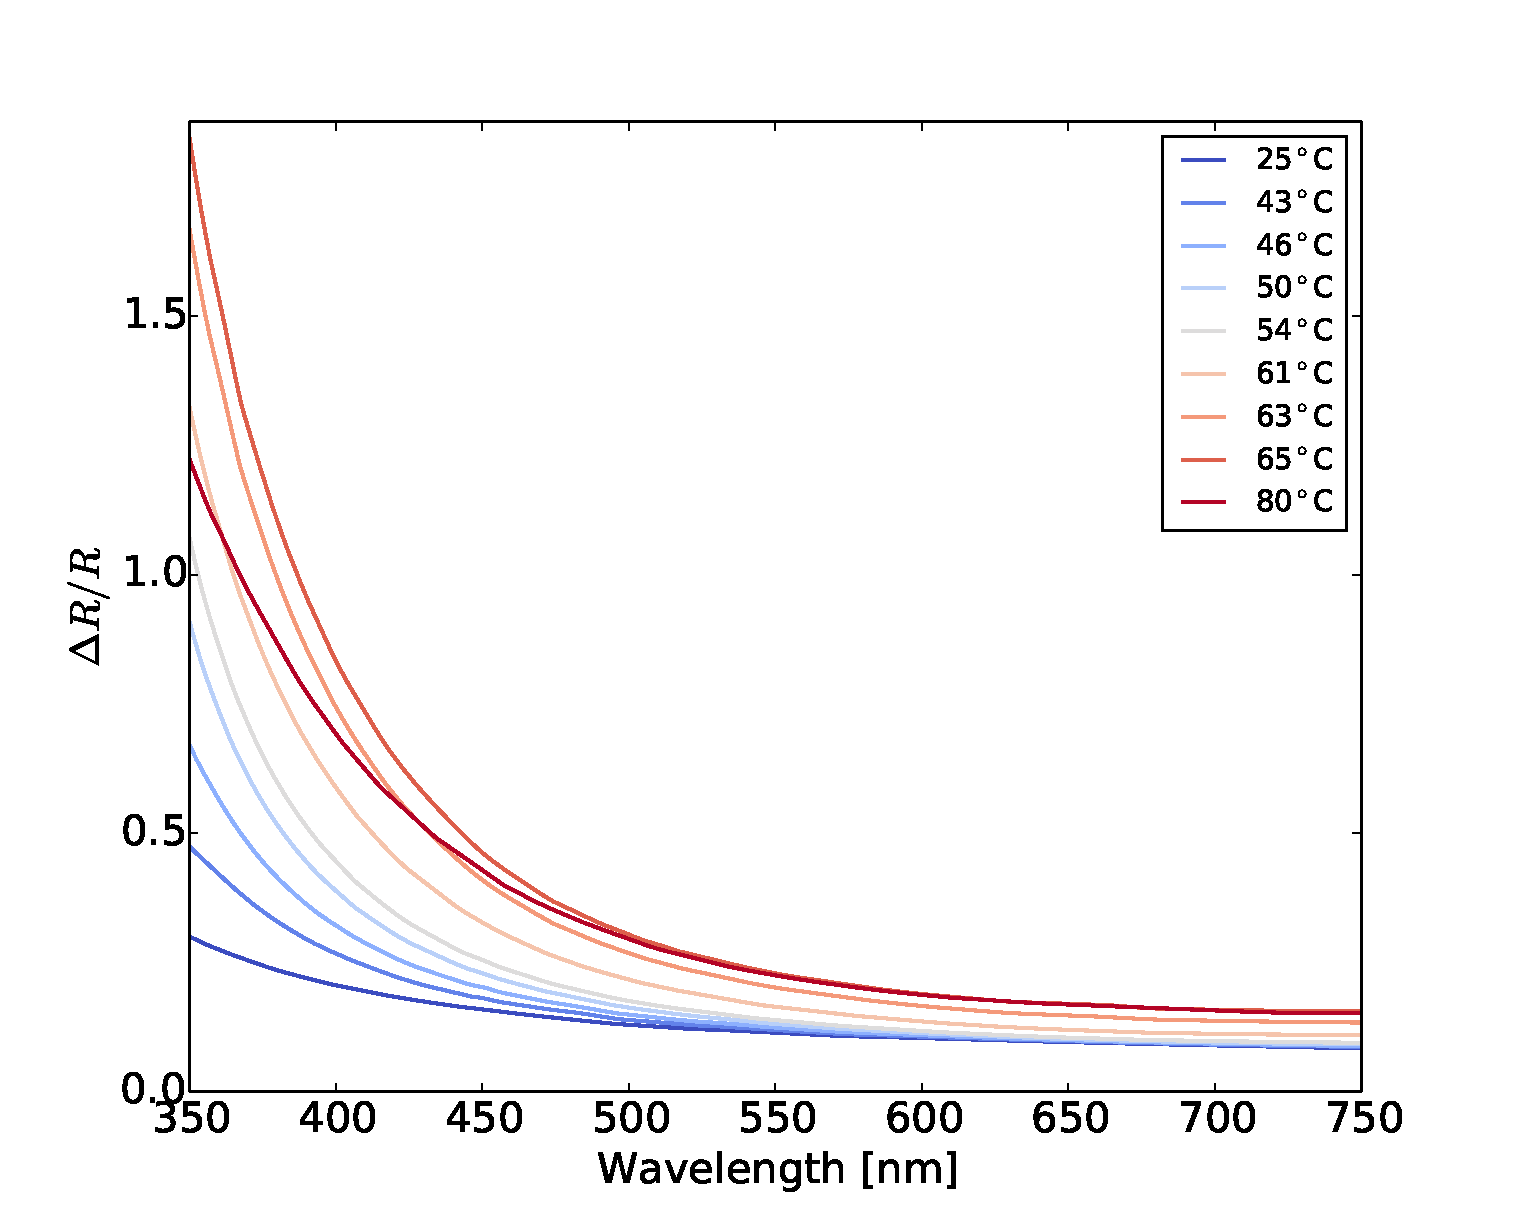
\includegraphics[width=\textwidth]{Results/Sim3/dR_visible.pdf}
        \caption{}
        %\label{fig:y equals x}
    \end{subfigure}
    %\hfill
    \begin{subfigure}[b]{0.3\textwidth}
        \centering
        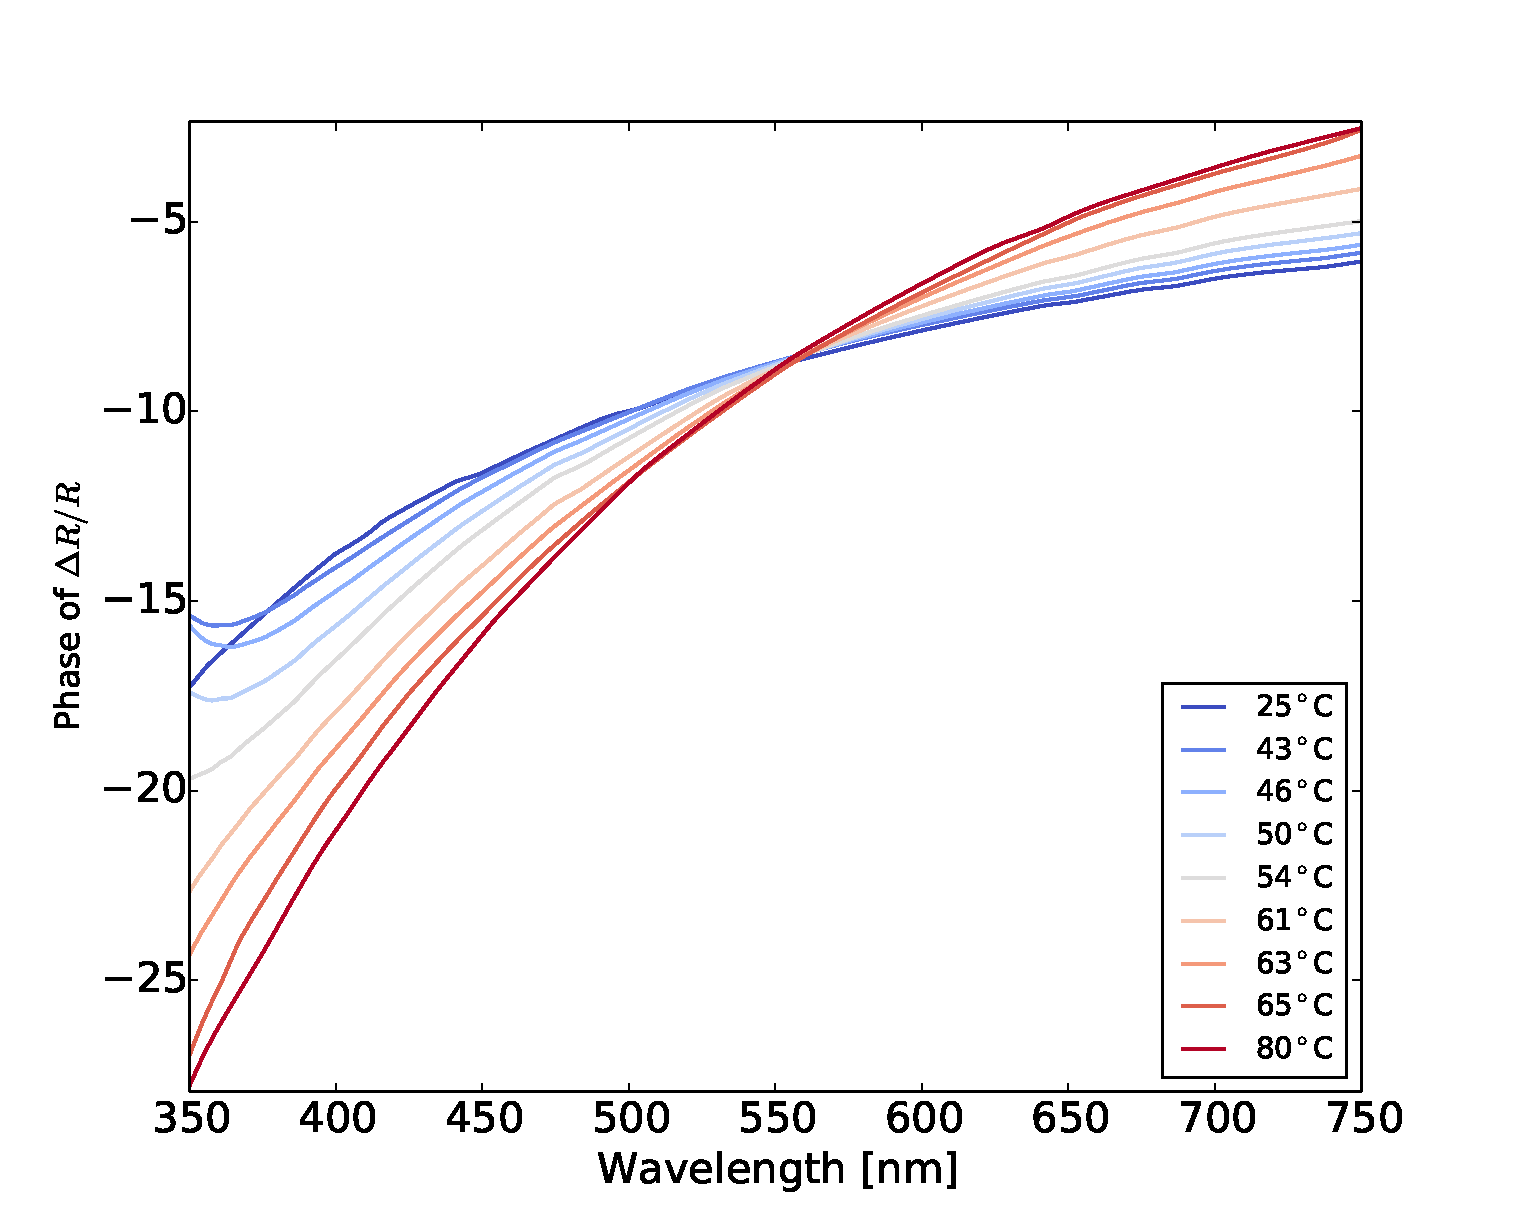
\includegraphics[width=\textwidth]{Results/Sim3/dRphase_visible.pdf}
        \caption{}
        %\label{fig:five over x}
    \end{subfigure}
    %\hfill
    \begin{subfigure}[b]{0.3\textwidth}
        \centering
        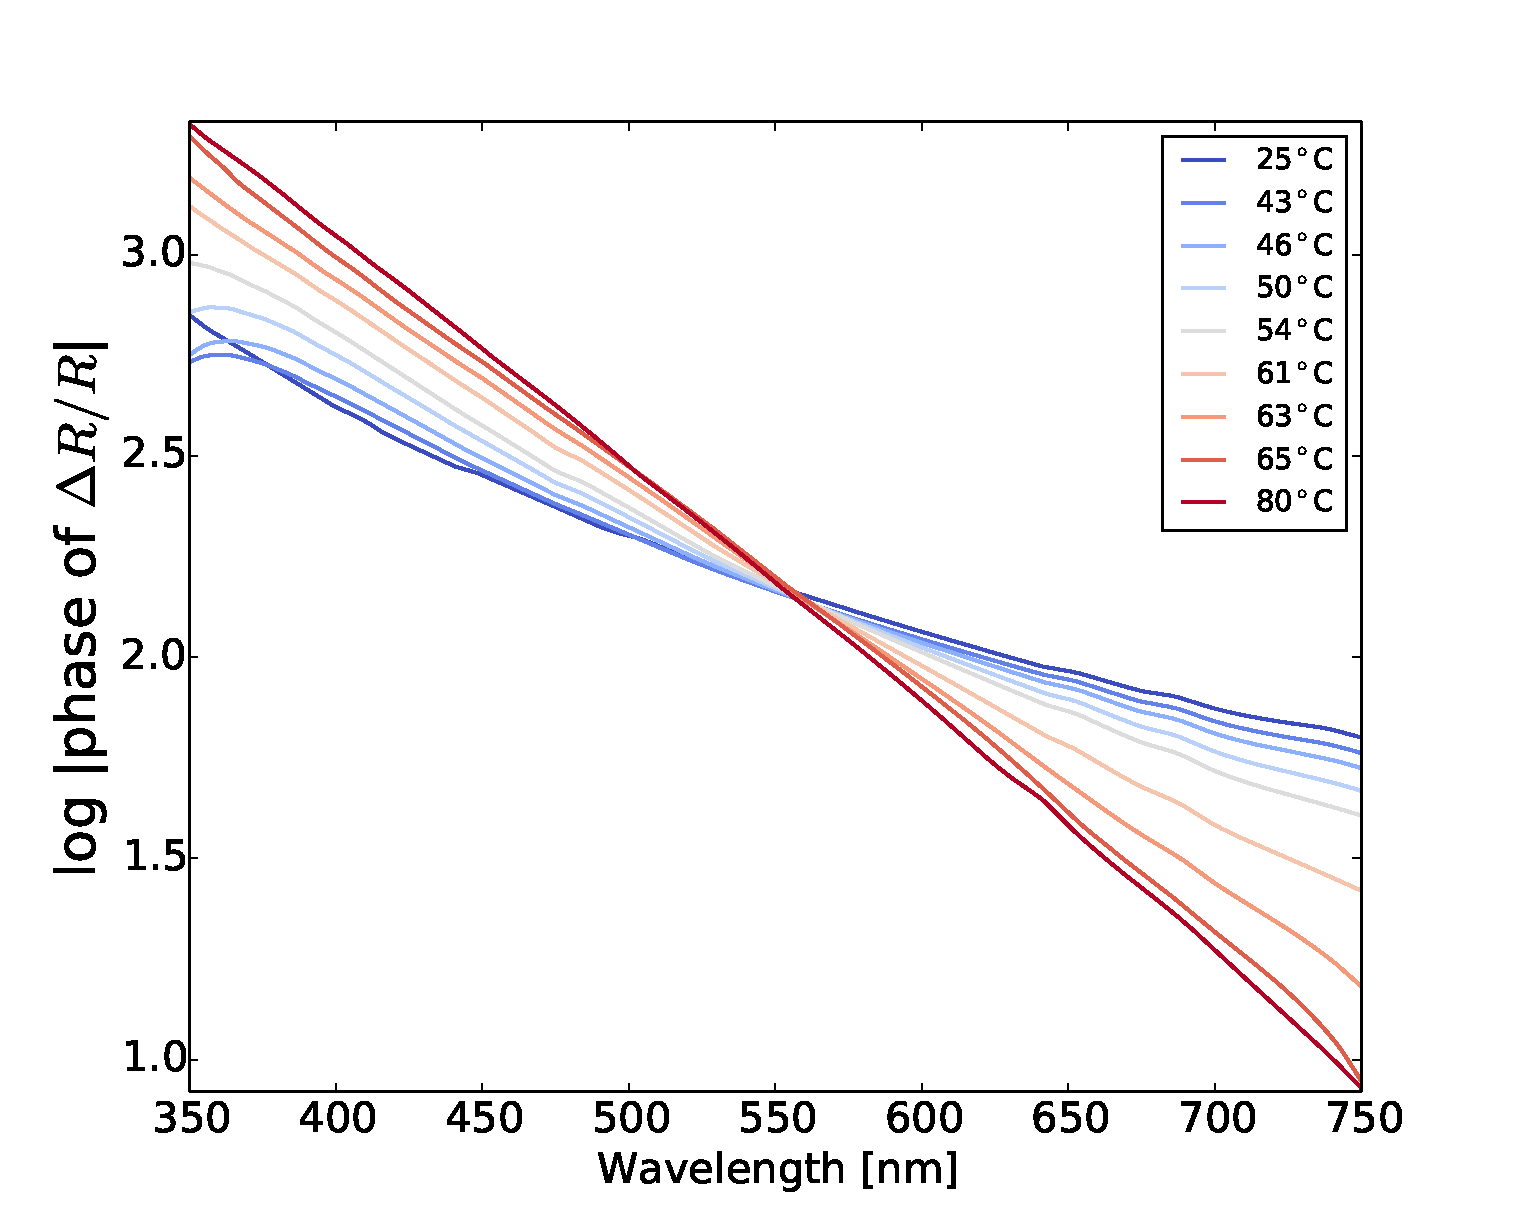
\includegraphics[width=\textwidth]{Results/Sim3/dRphase_visible_log.pdf}
        \caption{}
        %\label{fig:three sin x}
    \end{subfigure}
    \caption{R = 15nm, p-pol}
    %\label{fig:three graphs}
\end{figure}
%
\begin{figure}
    \centering
    \begin{subfigure}[b]{0.3\textwidth}
        \centering
        \includegraphics[width=\textwidth]{Results/Sim4/dR_visible.pdf}
        \caption{}
        %\label{fig:y equals x}
    \end{subfigure}
    %\hfill
    \begin{subfigure}[b]{0.3\textwidth}
        \centering
        \includegraphics[width=\textwidth]{Results/Sim4/dRphase_visible.pdf}
        \caption{}
        %\label{fig:five over x}
    \end{subfigure}
    %\hfill
    \begin{subfigure}[b]{0.3\textwidth}
        \centering
        \includegraphics[width=\textwidth]{Results/Sim4/dRphase_visible_log.pdf}
        \caption{}
        %\label{fig:three sin x}
    \end{subfigure}
    \caption{R = 15nm, s-pol}
    %\label{fig:three graphs}
\end{figure}
%
